%!TeX root=../main.tex

\chapter{Distribuzione e Prodotto finale}\label{ch:distribuzione-e-prodotto-finale}

\section{Strategia di distribuzione}\label{sec:strategia-di-distribuzione}
La fase di distribuzione ha avuto come obiettivo non solo il rilascio tecnico dell’applicazione, ma anche la validazione della sua utilizzabilità in un ambiente che simula condizioni reali di produzione.
Per \textbf{Swift Contest} è stato scelto un approccio multipiattaforma che copre i principali punti di accesso per i diversi tipi di utenti:
\begin{itemize}
    \item \textbf{Applicazione Web}: distribuita su \textbf{Vercel}, per garantire accessibilità universale da qualsiasi browser moderno, sia desktop che mobile.
    \item \textbf{Applicazione Android}: distribuita come pacchetto APK, reso disponibile tramite un meccanismo di download sicuro per un'esperienza d'uso ottimizzata su dispositivi mobili.
    \item \textbf{Infrastruttura Backend}: interamente gestita su \textbf{Supabase}, che ospita il database, lo storage, le funzioni serverless e i servizi realtime.
    \item \textbf{Pannello di Amministrazione}: sviluppato come strumento interno su \textbf{Retool} e interfacciato in modo sicuro con il backend, per le attività di moderazione e manutenzione.
\end{itemize}
Questa strategia ibrida consente di bilanciare la facilità di accesso (garantita dalla versione Web) con un'esperienza d'uso ottimizzata (offerta dalla versione Android), mantenendo al contempo un backend centralizzato, sicuro e scalabile.

\begin{figure}[H]
    \centering
    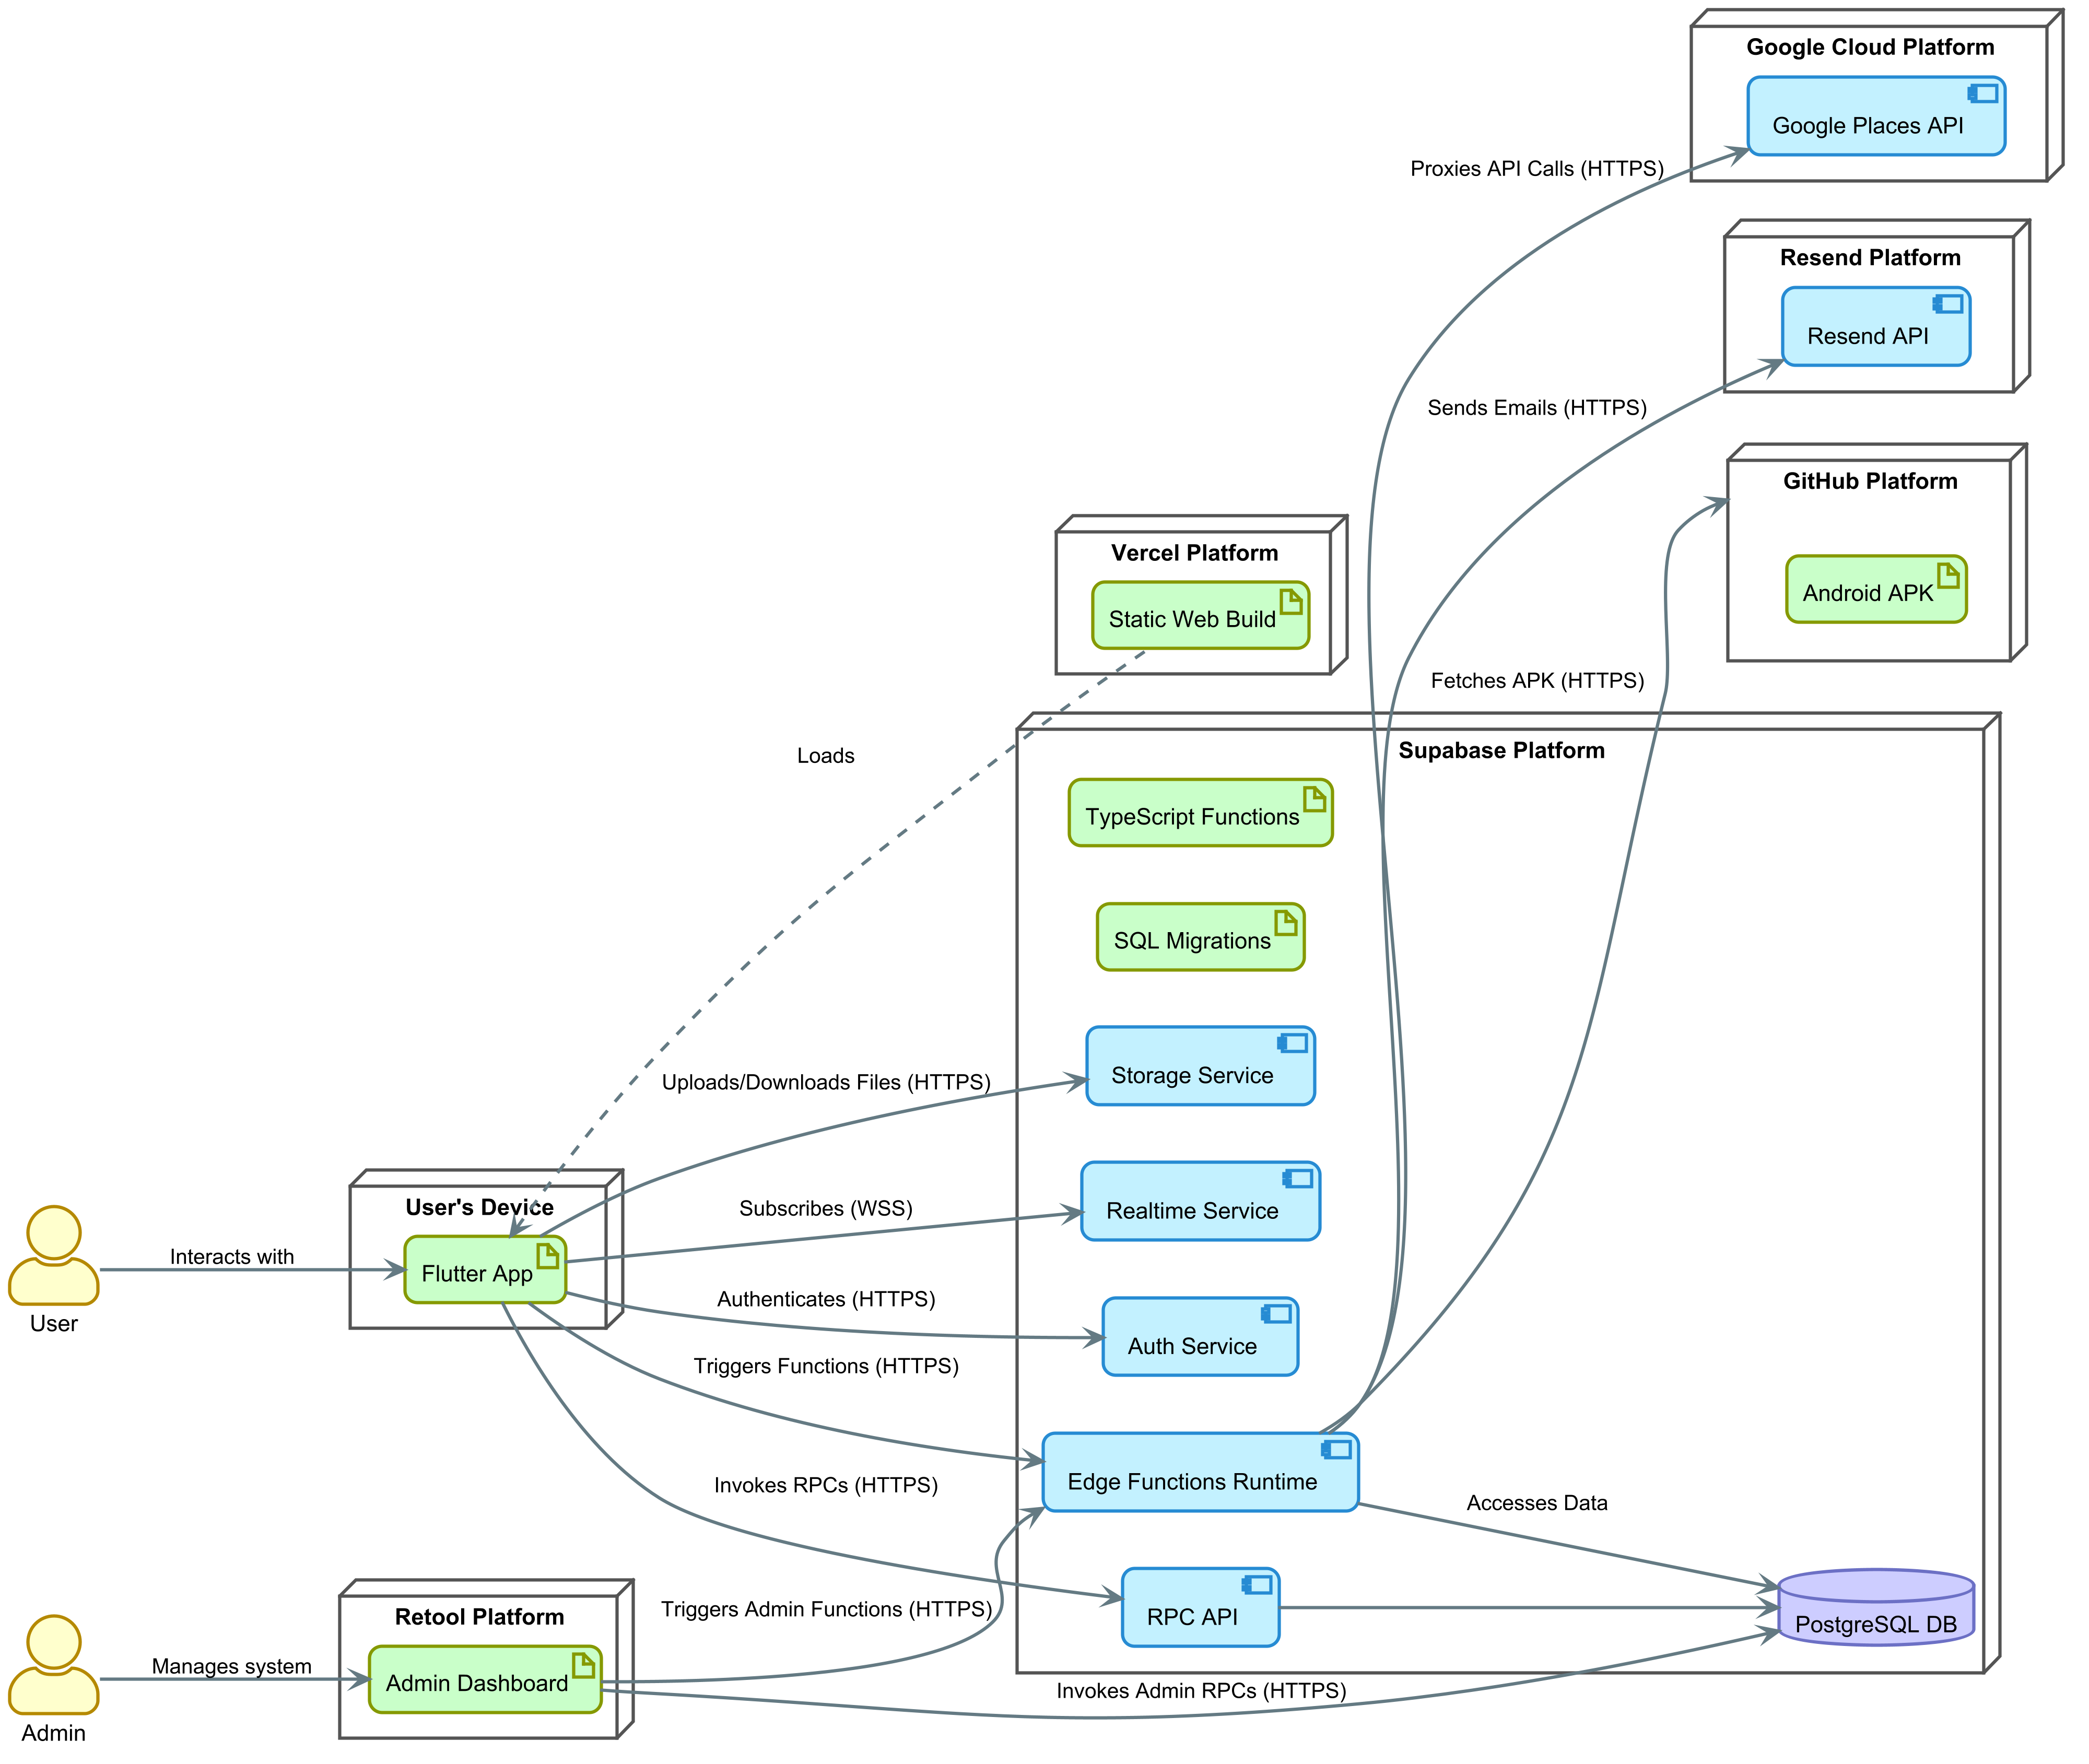
\includegraphics[width=\textwidth]{diagrammi/deployment-diagram}
    \caption{Diagramma di Deployment dell'architettura completa di Swift Contest.}
    \label{fig:deployment_diagram}
\end{figure}

\section{Distribuzione Web su Vercel}\label{sec:distribuzione-web-su-vercel}
La versione Web dell'applicazione Flutter è stata distribuita su Vercel, una piattaforma serverless ottimizzata per la distribuzione di frontend moderni.
Il processo è completamente automatizzato tramite una pipeline di CI/CD (Continuous Integration/Continuous Deployment) integrata con il repository Git del progetto.
Ogni \emph{push} sul branch \texttt{main} innesca automaticamente una nuova build dell'applicazione Flutter in modalità \emph{release} e un conseguente deploy sulla piattaforma.

Per garantire il corretto funzionamento di una Single Page Application (SPA) come Flutter Web, è stato configurato un file \texttt{vercel.json} che gestisce il rewrite di tutte le rotte verso il file \texttt{index.html}, permettendo al router di Flutter (\texttt{auto\_route}) di gestire la navigazione lato client.

\section{Distribuzione Android}\label{sec:distribuzione-android}
Per la piattaforma Android, è stata prodotta una \textbf{release in formato APK}.
Data la natura prototipale del progetto, si è evitato il complesso processo di pubblicazione sul Google Play Store, optando per un approccio di distribuzione controllata che garantisce comunque sicurezza e facilità di aggiornamento:
\begin{enumerate}
    \item L'APK viene caricato come \emph{release asset} su un repository GitHub privato.
    \item Un'apposita Edge Function, \texttt{get-latest-apk}, è stata creata su Supabase per fungere da proxy sicuro.
    Questa funzione utilizza un Personal Access Token (PAT) di GitHub, memorizzato in modo sicuro in Supabase, per autenticarsi all'API di GitHub e scaricare l'asset.
    \item L'applicazione web offre un pulsante ``Download for Android'' che invoca questa Edge Function.
    L'utente riceve così l'ultima versione dell'APK direttamente dal backend, senza che il repository GitHub o le credenziali di accesso vengano mai esposte.
\end{enumerate}

\begin{figure}[H]
    \centering
    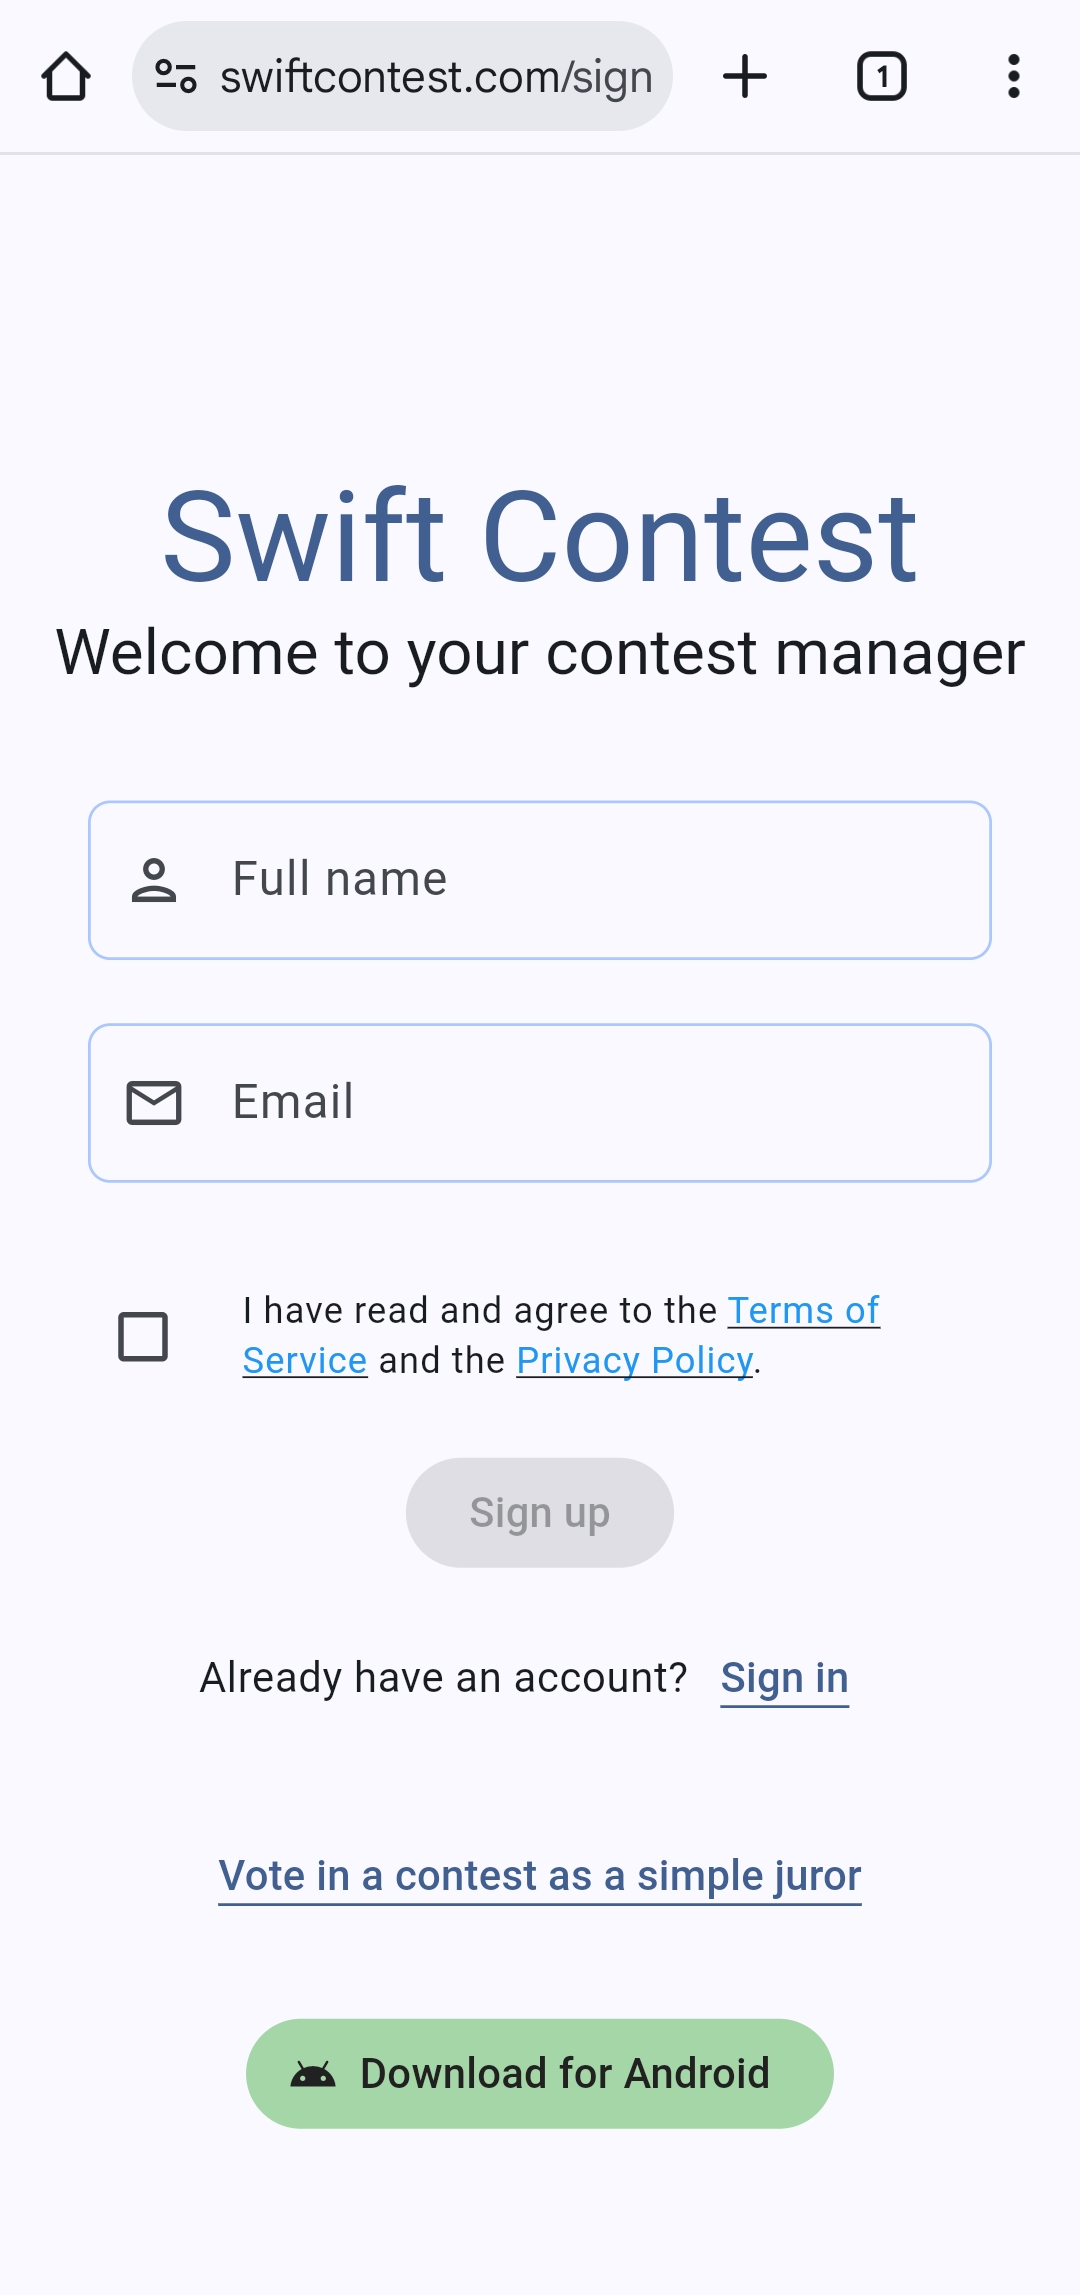
\includegraphics[width=0.30\textwidth]{figure/web-sign-up}
    \caption{Pagina di accesso dell'applicazione web distribuita su Vercel.}
    \label{fig:web-sign-up}
\end{figure}

\section{Backend e Supabase}\label{sec:backend-e-supabase}
L'intera infrastruttura backend è gestita su Supabase.
Il processo di deployment del database è basato su migrazioni SQL, seguendo le pratiche di \textbf{Infrastructure as Code (IaC)}.
Ogni modifica allo schema del database, alle policy RLS o alle funzioni RPC è definita in un file \texttt{.sql} all'interno della cartella \texttt{supabase/migrations}.
La CLI di Supabase viene utilizzata per applicare queste migrazioni in modo sequenziale e versionato, garantendo che l'ambiente di produzione sia sempre allineato con la definizione del codice.
Le Edge Functions, scritte in TypeScript, vengono anch'esse deployate tramite la CLI\@.

% Tabella riassuntiva delle componenti Supabase
\begin{longtable}{p{0.2\textwidth} p{0.45\textwidth} p{0.3\textwidth}}
    \toprule
    \textbf{Componente} & \textbf{Utilizzo nel Progetto Swift Contest} & \textbf{Implementazione / Note Tecniche} \\
    \midrule
    \endfirsthead
    \toprule
    \textbf{Componente} & \textbf{Utilizzo nel Progetto Swift Contest} & \textbf{Implementazione / Note Tecniche} \\
    \midrule
    \endhead

    \textbf{Database} \newline (PostgreSQL) &
    Persistenza di tutti i dati applicativi: utenti, contest, partecipazioni, giurie, voti, ecc.
    È il ``single source of truth'' del sistema.
    &
    Schema e logica definiti tramite file di migrazione SQL nella cartella \texttt{supabase/migrations}. \\
    \midrule

    \textbf{Auth} &
    Gestione completa del ciclo di vita degli utenti: registrazione, login (email/password), autenticazione anonima per i giurati semplici e gestione delle sessioni tramite JWT. &
    Integrato tramite la libreria \texttt{supabase-flutter}.
    La tabella \texttt{auth.users} è estesa dalla tabella \texttt{public.profiles}. \\
    \midrule

    \textbf{Storage} &
    Archiviazione sicura di tutti i file binari caricati dagli utenti, come le immagini dei contest e i file dei \emph{Work}. &
    Nessun file è pubblico.
    L'accesso avviene esclusivamente tramite \emph{signed URL} temporanei generati lato server. \\
    \midrule

    \textbf{Edge Functions} &
    Esecuzione di logica server-side complessa, orchestrazione di operazioni multi-servizio (es.\ cancellazione utente da DB e Storage) e interazione con API esterne (Resend, Google Places).
    &
    Scritte in TypeScript (runtime Deno) e deployate dalla cartella \texttt{supabase/functions}. \\
    \midrule

    \textbf{Funzioni RPC} &
    Punto di ingresso primario per la logica di business confinata al database.
    Utilizzate per la maggior parte delle operazioni CRUD. &
    Scritte in PL/pgSQL e definite nei file di migrazione. \\
    \midrule

    \textbf{Realtime} &
    Propagazione di modifiche del database ai client sottoscritti in tempo reale.
    Utilizzato per le notifiche della \textbf{inbox} (tabella \texttt{messages}) e per aggiornare lo stato delle sessioni di voto.
    &
    L'autorizzazione alla sottoscrizione è gestita tramite policy RLS di tipo \texttt{SELECT}. \\

    \bottomrule \\
    \caption{Riepilogo delle componenti Supabase e del loro utilizzo nel progetto.}
    \label{tab:supabase_components}
\end{longtable}

\section{Dashboard amministrativa (Retool)}\label{sec:dashboard-amministrativa-(retool)}
Per le attività di amministrazione avanzata, come la moderazione degli utenti e la gestione dei contenuti, è stata creata una dashboard interna utilizzando \textbf{Retool}.
Questa interfaccia, non esposta agli utenti finali, comunica con il backend Supabase attraverso l'API sicura descritta nel capitolo precedente, utilizzando un utente di database dedicato per le letture ed Edge Functions protette da API-Key per le operazioni di scrittura.

\begin{figure}[H]
    \centering
    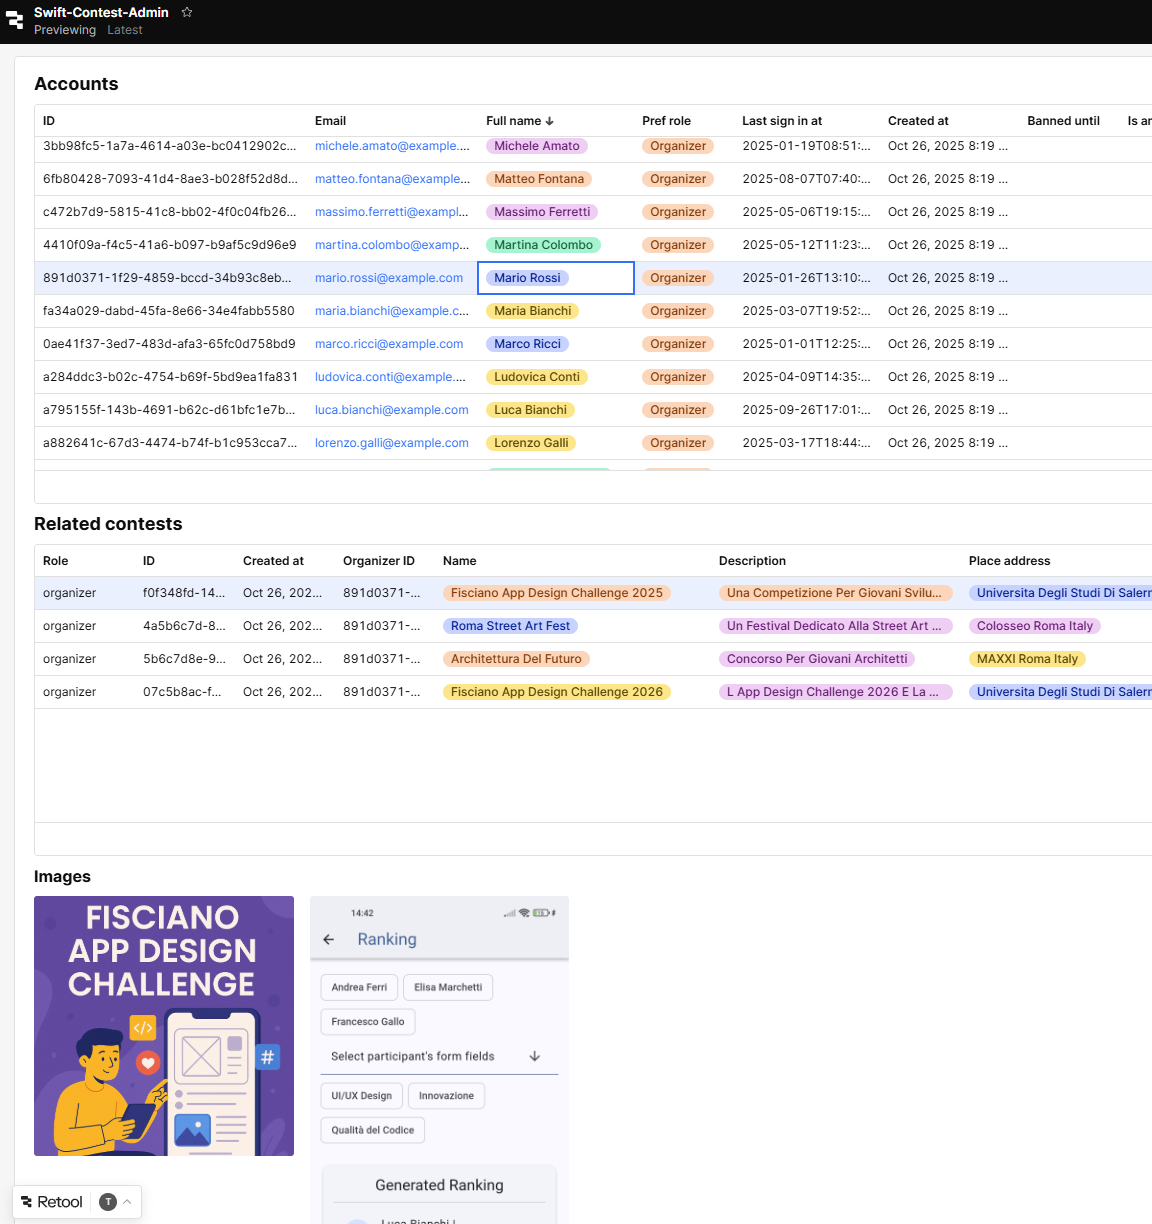
\includegraphics[width=0.6\textwidth]{figure/retool-dashboard}
    \caption{La dashboard di amministrazione sviluppata in Retool.}
    \label{fig:retool-dashboard}
\end{figure}

\section{Prodotto finale: Interfaccia Utente e Flussi Operativi}\label{sec:prodotto-finale}
In questa sezione viene presentato il prodotto finale attraverso un'analisi visuale dei suoi \textbf{flussi operativi principali}.
L'obiettivo non è quello di documentare ogni singola schermata dell'applicazione, ma di illustrare, tramite l'interfaccia utente (UI), i percorsi più significativi per ciascuno degli attori del sistema.

Partendo dalle schermate di base, come l'autenticazione e le impostazioni, verranno poi illustrati i flussi specifici per l'\textbf{Organizzatore}, il \textbf{Partecipante}, il \textbf{Giurato Nominato} e il \textbf{Giurato Semplice} (ospite).

\subsection{Accesso e Autenticazione}\label{subsec:accesso-e-autenticazione}
L'accesso all'applicazione inizia con una \textbf{Splash Screen} che gestisce l'inizializzazione dei servizi principali.
Successivamente, l'utente viene indirizzato al flusso di autenticazione, che comprende le pagine di \textbf{Sign In} (per l'accesso), \textbf{Sign Up} (per la registrazione di un nuovo account) e le relative schermate per la verifica dell'email.
L'interfaccia è stata progettata per essere pulita, minimale e coerente con le linee guida del Material Design 3.

% --- Esempio con immagini affiancate (CONSIGLIATO) ---
\begin{figure}[H]
    \centering
    \begin{minipage}[t]{0.30\textwidth}
        \centering
        
\includegraphics[width=\linewidth]{figure/splash}
        \subcaption{Splash Screen}
        \label{fig:splash}
    \end{minipage}\hfill
    \begin{minipage}[t]{0.30\textwidth}
        \centering
        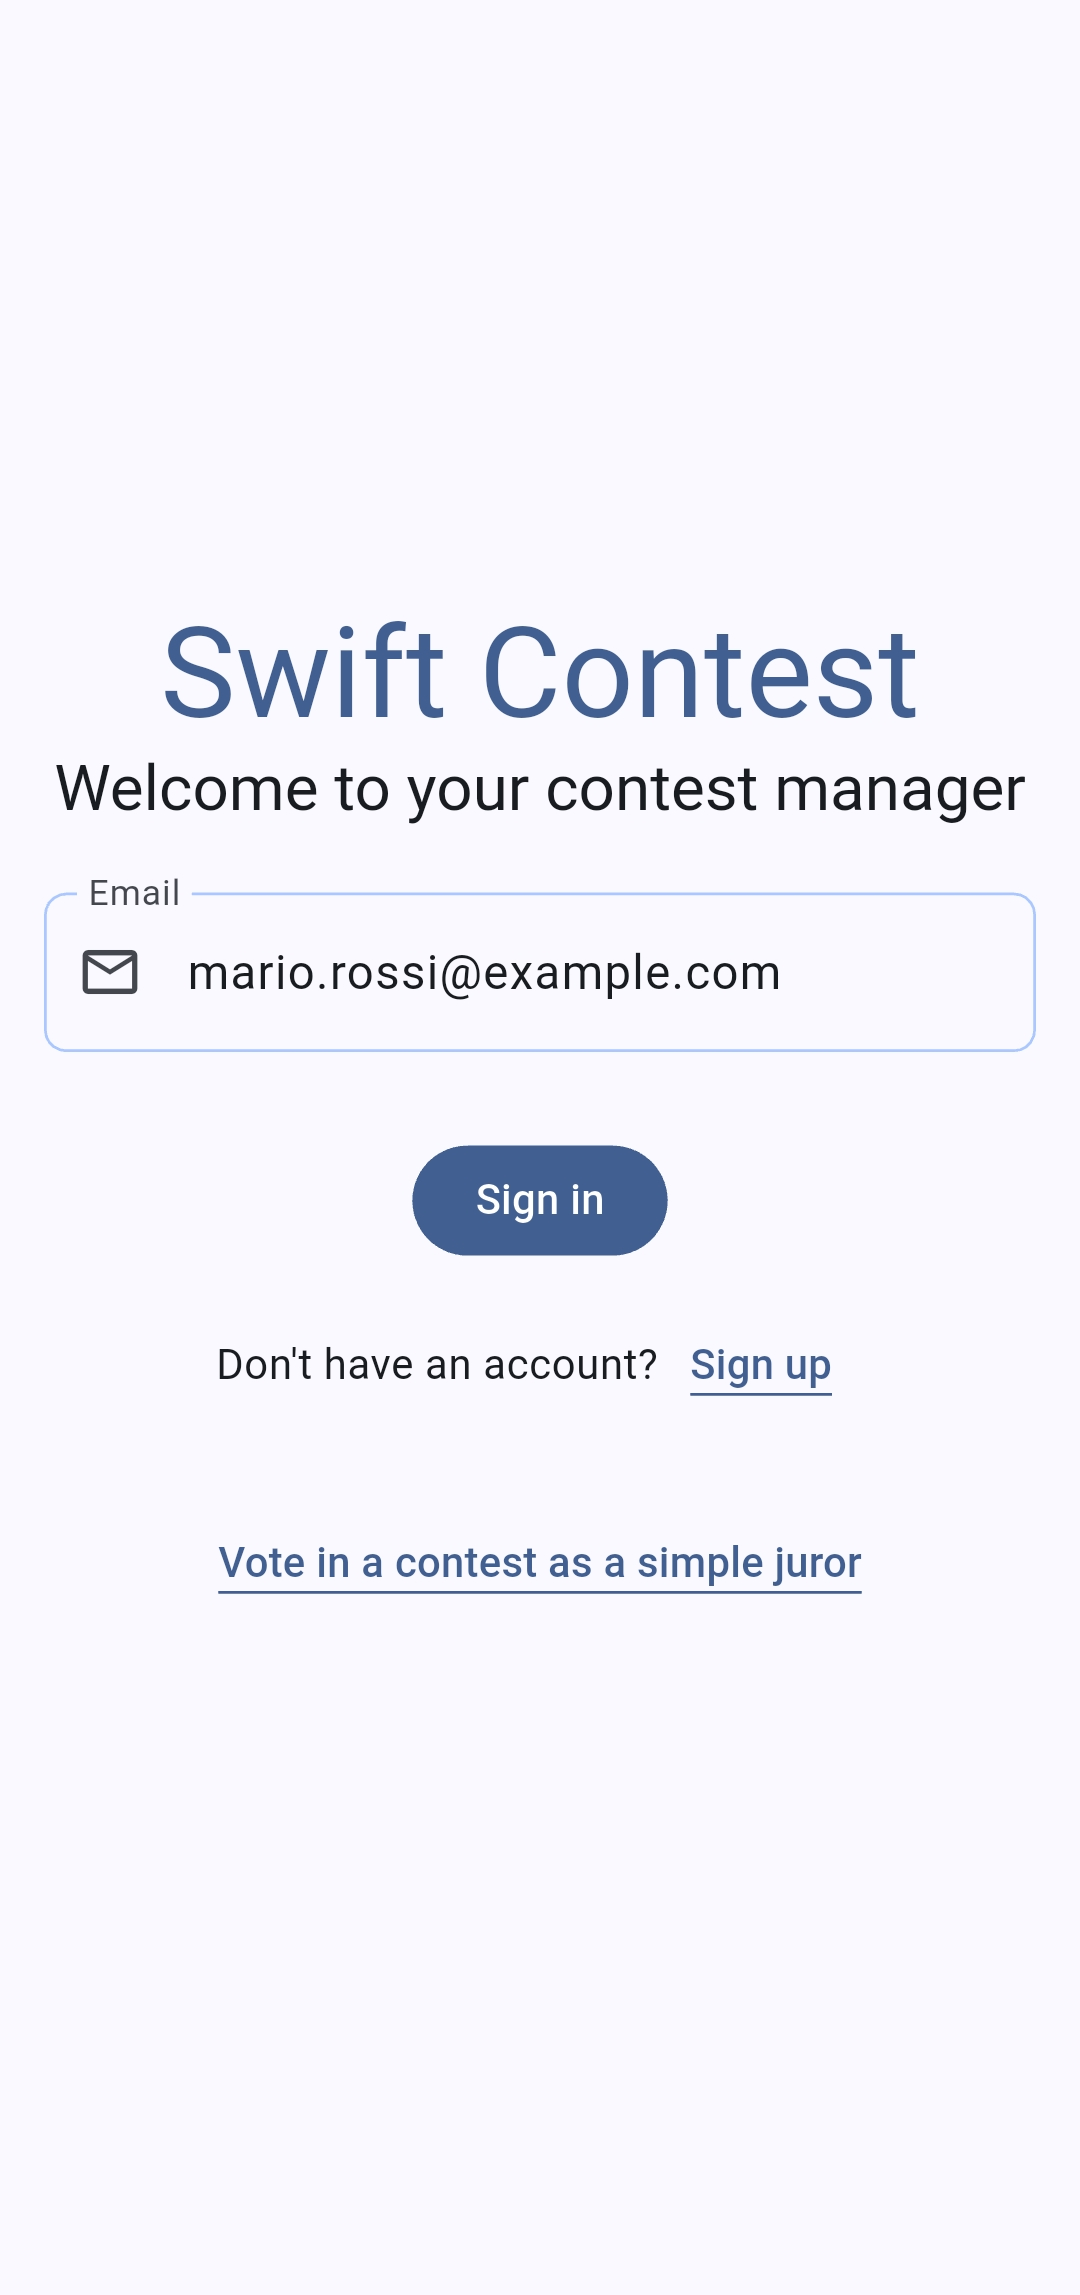
\includegraphics[width=\linewidth]{figure/sign-in}
        \subcaption{Pagina di Sign In}
        \label{fig:signin}
    \end{minipage}\hfill
    \begin{minipage}[t]{0.30\textwidth}
        \centering
        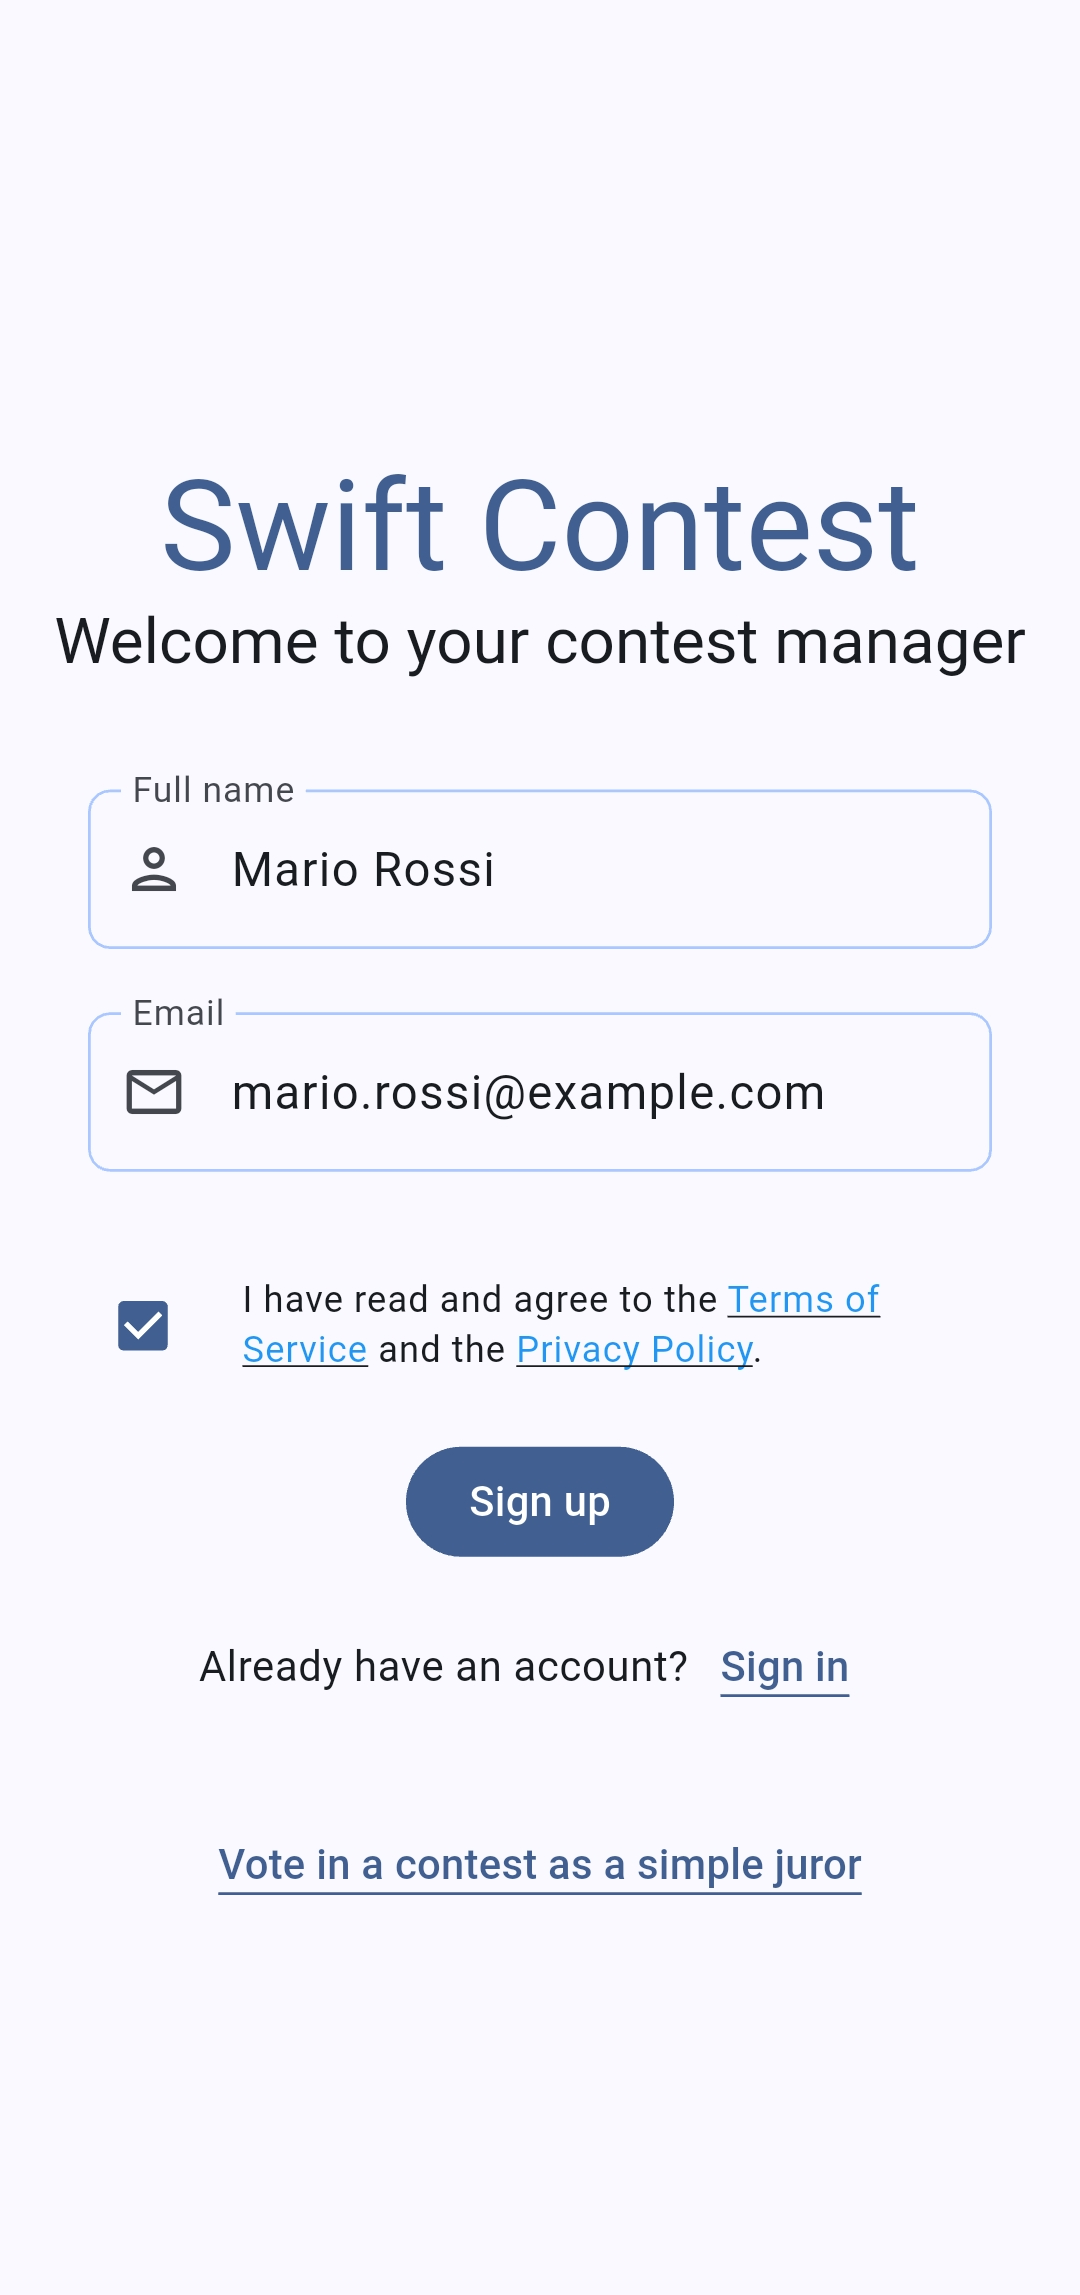
\includegraphics[width=\linewidth]{figure/sign-up}
        \subcaption{Pagina di Sign Up}
        \label{fig:signup}
    \end{minipage}
    \caption{Le schermate del flusso di autenticazione dell'applicazione.}
    \label{fig:auth-flow}
\end{figure}

\subsection{Gestione delle Impostazioni}\label{subsec:gestione-impostazioni}
Una volta autenticato, ogni utente ha accesso a una sezione dedicata alle impostazioni.
Da qui, l'utente può navigare alla pagina \textbf{Impostazioni Account}, dove può modificare i dati del proprio profilo (come il nome completo) o procedere con l'eliminazione sicura e autonoma del proprio account.

\begin{figure}[H]
    \centering
    \begin{minipage}[t]{0.30\textwidth}
        \centering
        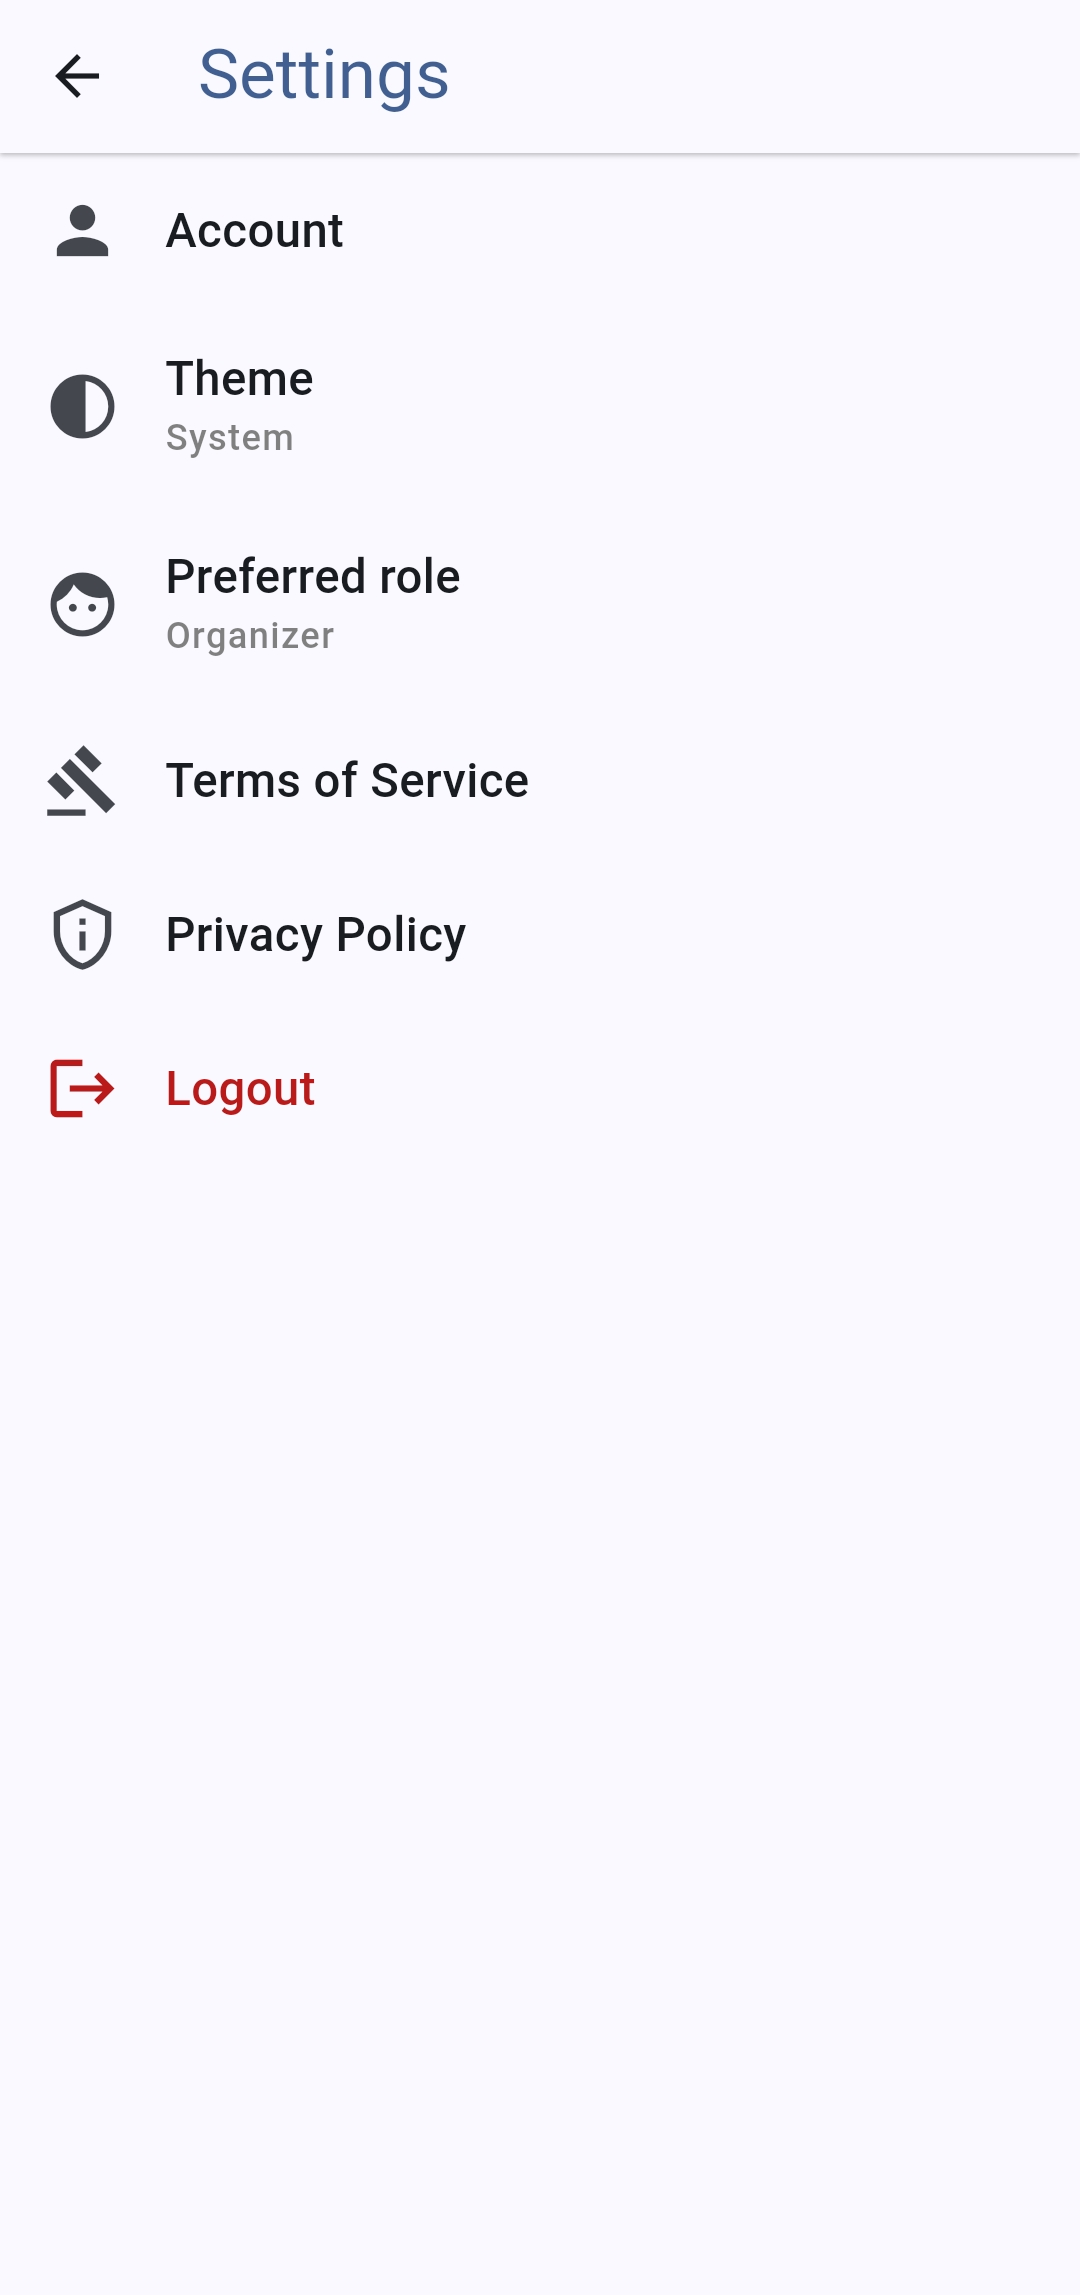
\includegraphics[width=\linewidth]{figure/settings}
        \subcaption{Pagina delle Impostazioni Generali}
        \label{fig:settings}
    \end{minipage}
    \quad
    \begin{minipage}[t]{0.30\textwidth}
        \centering
        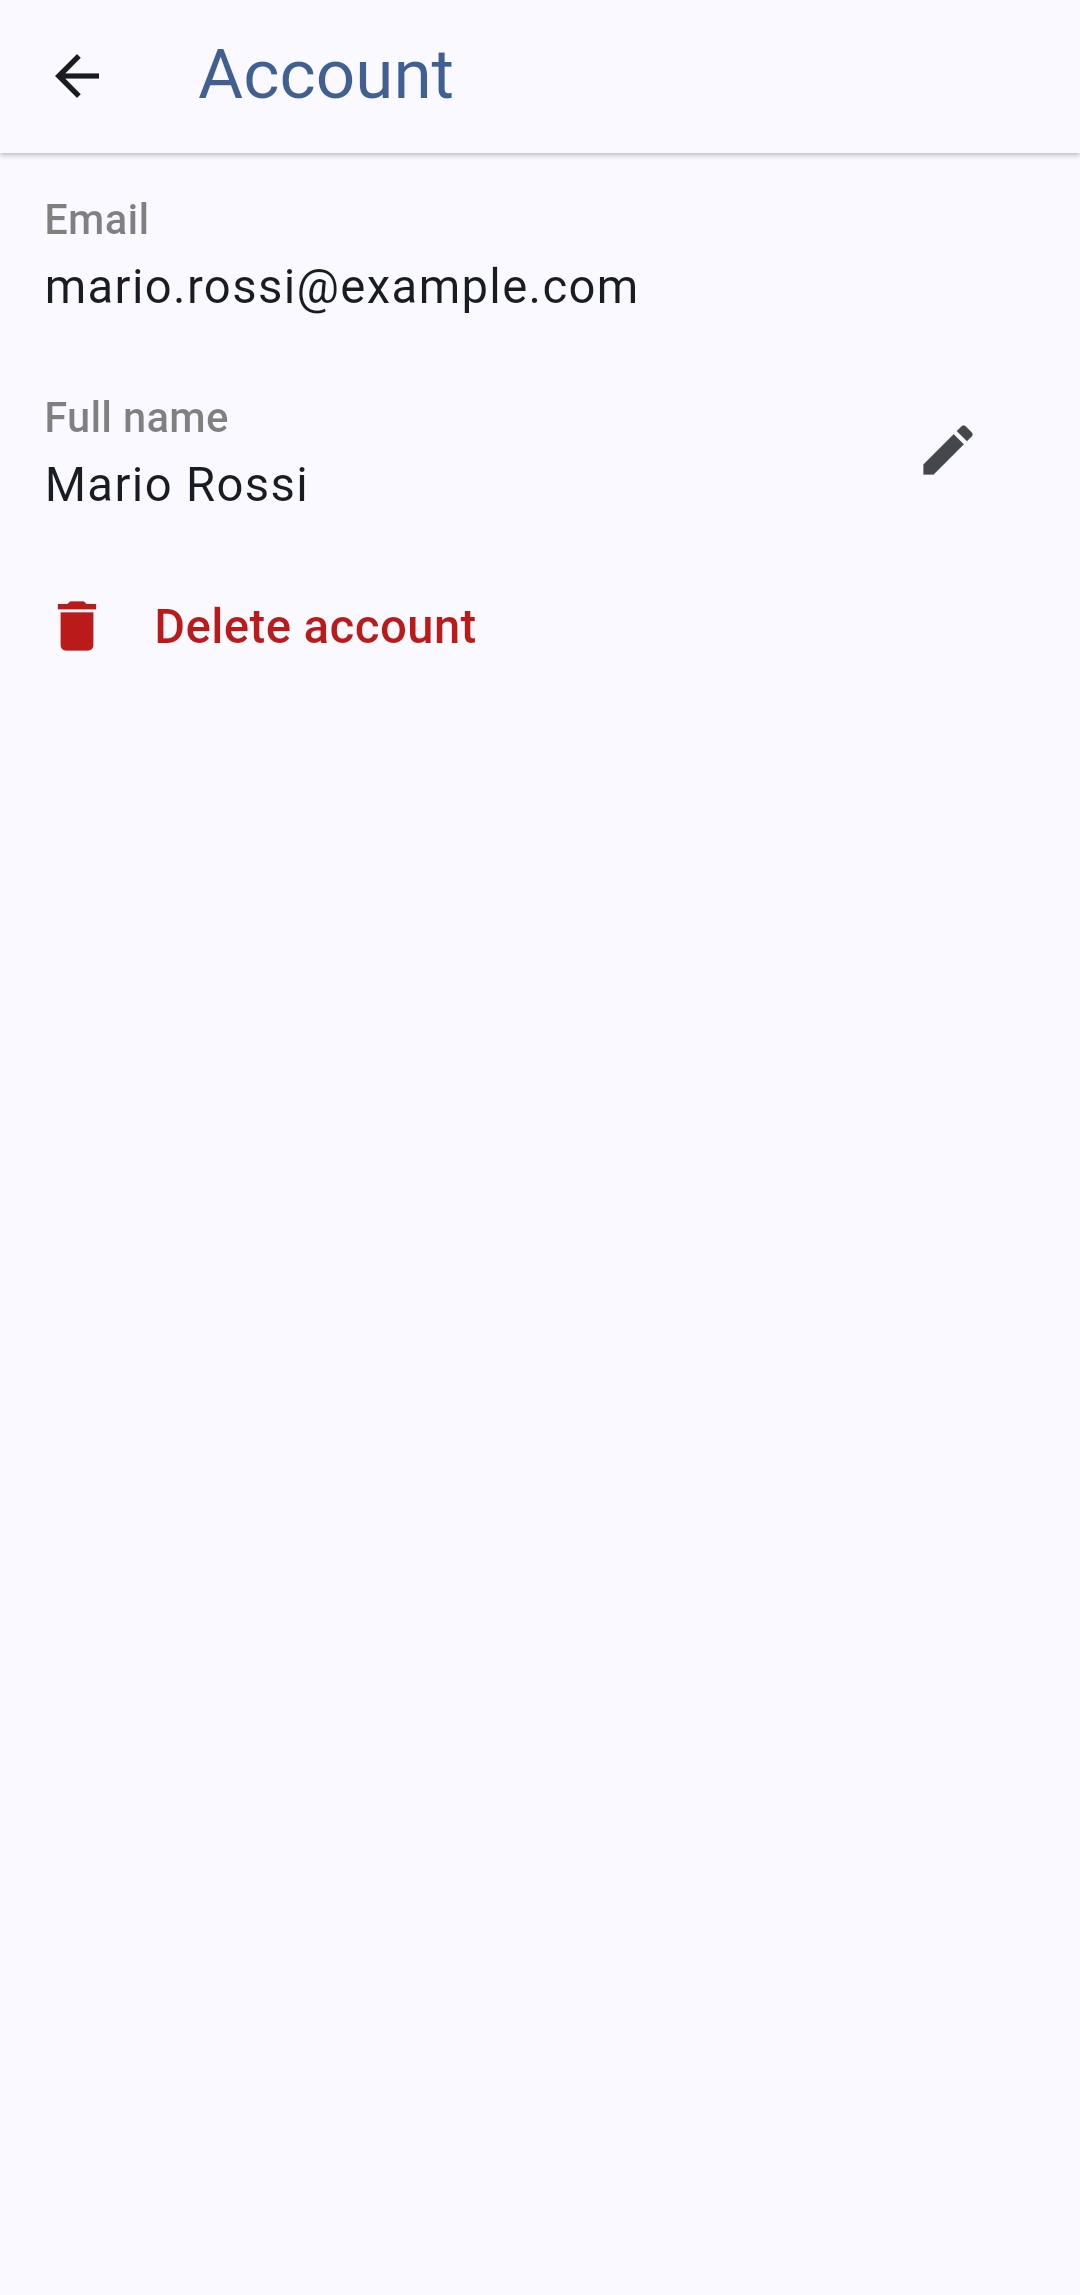
\includegraphics[width=\linewidth]{figure/account-settings}
        \subcaption{Pagina Impostazioni Account}
        \label{fig:account_settings}
    \end{minipage}
    \caption{Le schermate per la gestione delle impostazioni dell'app e dell'account utente.}
    \label{fig:settings-flow}
\end{figure}

\subsection{Flusso dell'Organizzatore}\label{subsec:flusso-organizzatore}
L'organizzatore è l'attore con il set di funzionalità più ricco, responsabile dell'intero ciclo di vita del contest.
Il suo percorso inizia dalla \textbf{Home Page}, che funge da dashboard principale, mostrando l'elenco dei contest da lui creati e fornendo l'accesso a tutte le funzionalità principali.

% --- FIGURA: Home Page Organizzatore ---
\begin{figure}[H]
    \centering
    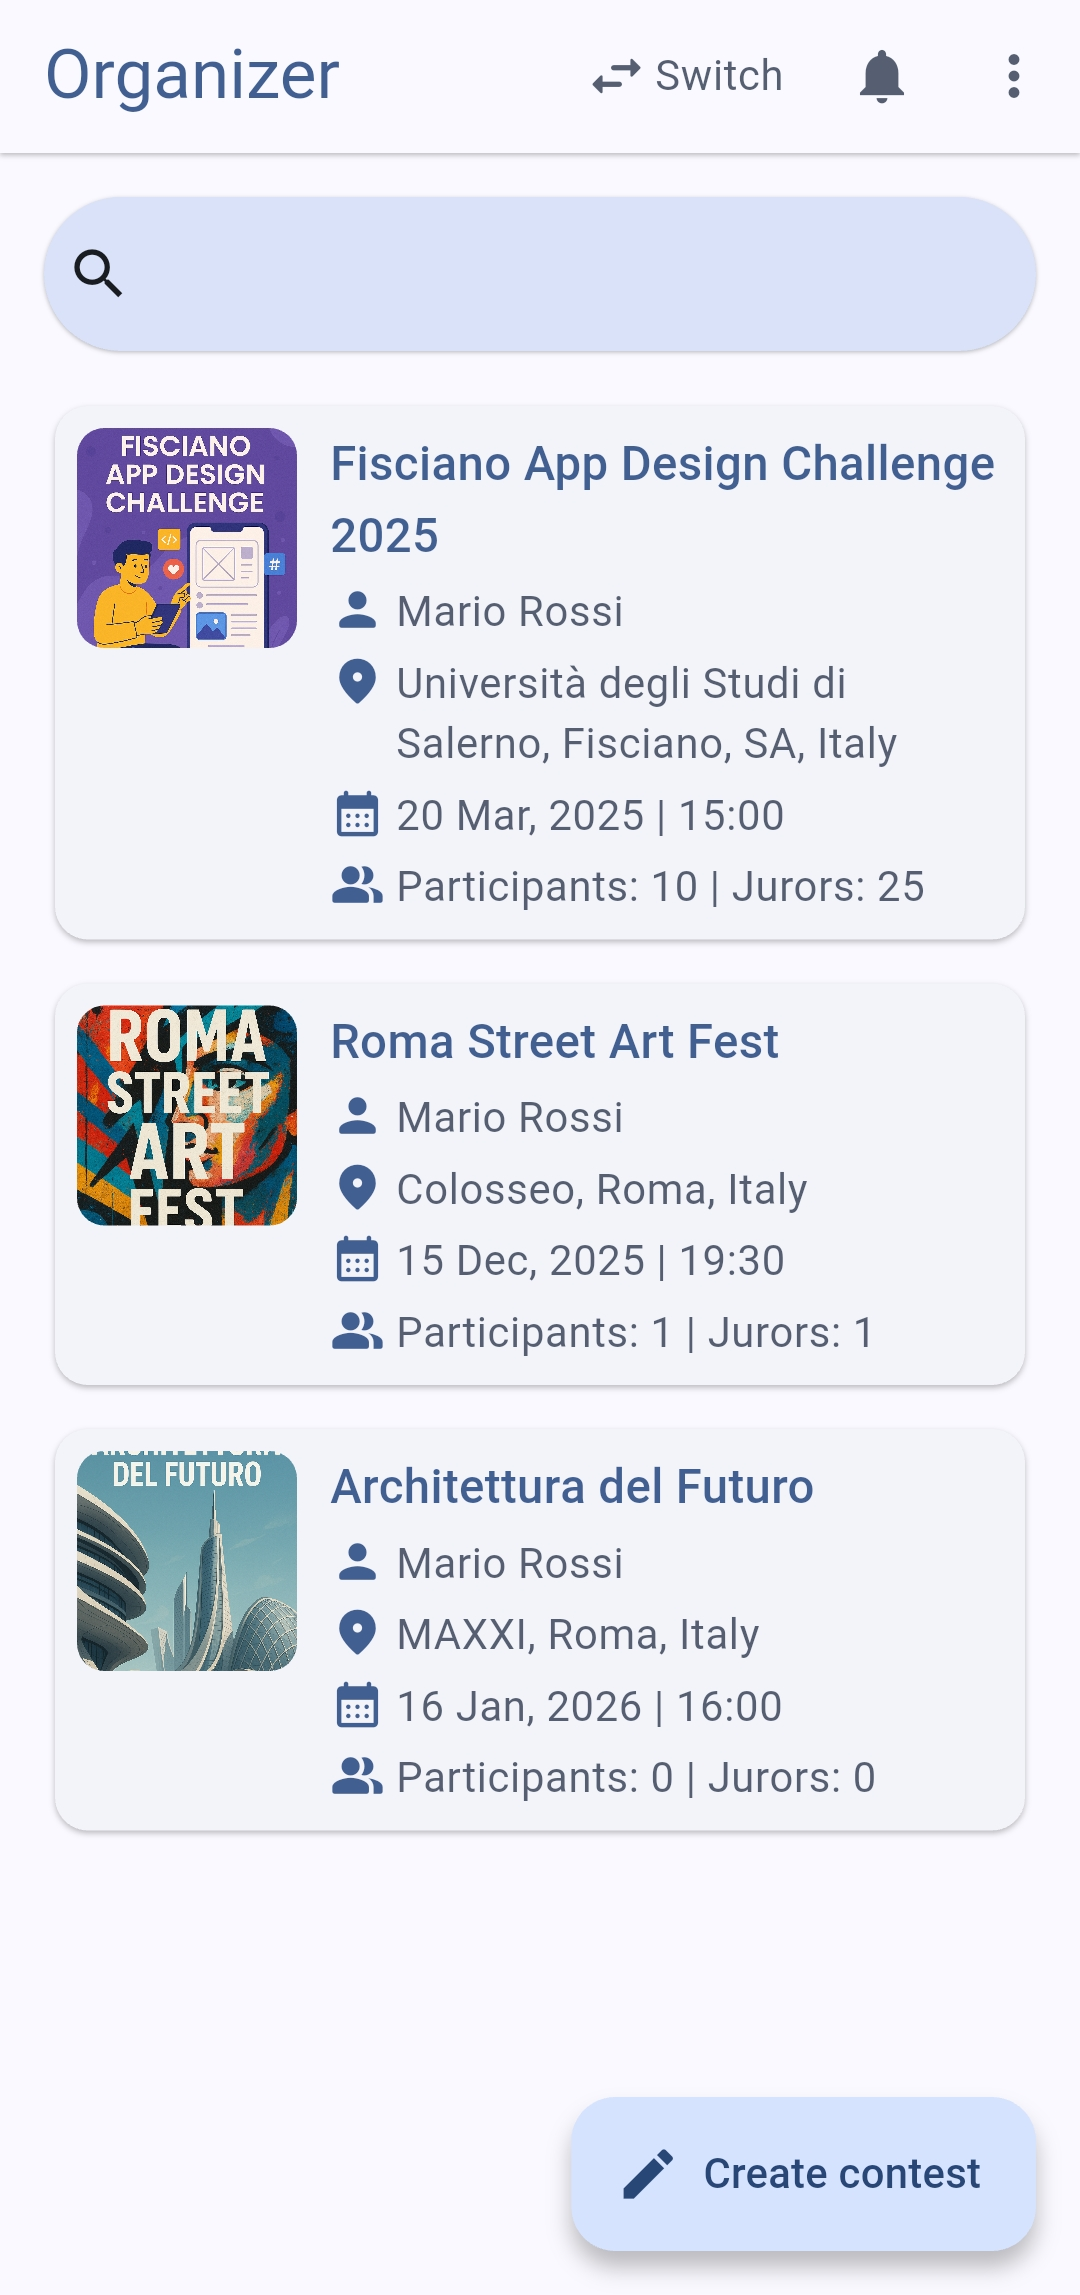
\includegraphics[width=0.4\textwidth]{figure/organizer-home}
    \caption{La Home Page dell'Organizzatore, con l'elenco dei contest gestiti.}
    \label{fig:organizer_home}
\end{figure}

\paragraph{Creazione di un Nuovo Contest}
Dalla home page, l'organizzatore può avviare la creazione di un nuovo contest.
Viene guidato attraverso un \textbf{form multi-step} che semplifica l'inserimento di tutte le informazioni necessarie, suddivise in tre passaggi logici:
\begin{enumerate}
    \item \textbf{Dati Principali}: inserimento di nome, descrizione, data e luogo del contest.
    La selezione del luogo è assistita da un'interfaccia integrata con l'API di Google Places.
    \item \textbf{Immagini}: caricamento delle immagini rappresentative che verranno utilizzate come copertina per la pagina del contest.
    \item \textbf{Periodo di Sottomissione}: definizione della data di inizio e di fine per la sottomissione dei lavori da parte dei partecipanti.
\end{enumerate}
Una volta completato, il nuovo contest appare nella sua dashboard, pronto per essere configurato.

% --- FIGURE: Creazione Contest (3 immagini affiancate) ---
\begin{figure}[H]
    \centering
    \begin{minipage}[t]{0.30\textwidth}
        \centering
        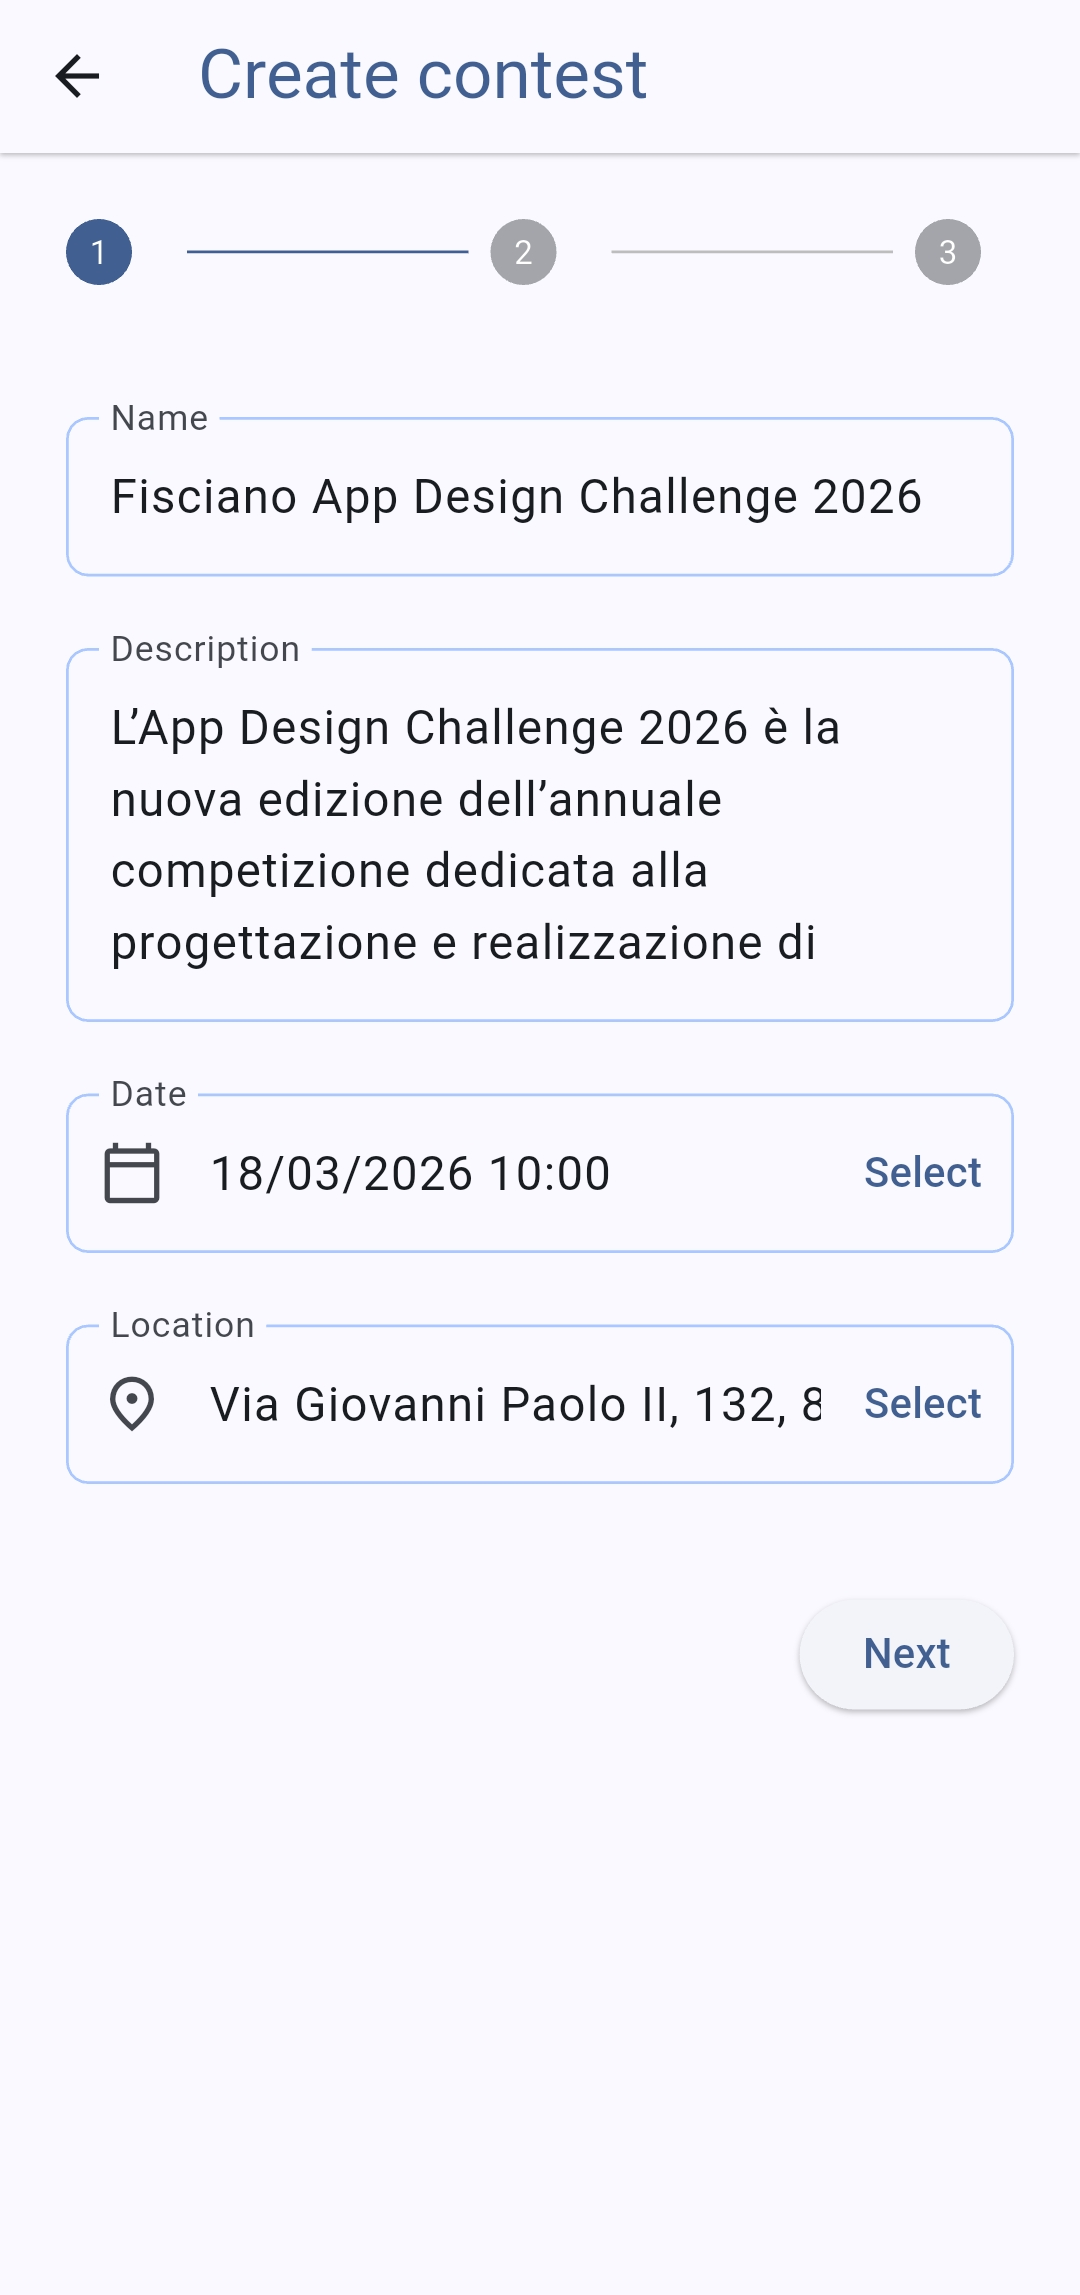
\includegraphics[width=\linewidth]{figure/organizer-create-contest-step1}
        \subcaption{Passo 1: Dati Principali}
        \label{fig:create_contest_1}
    \end{minipage}\hfill
    \begin{minipage}[t]{0.30\textwidth}
        \centering
        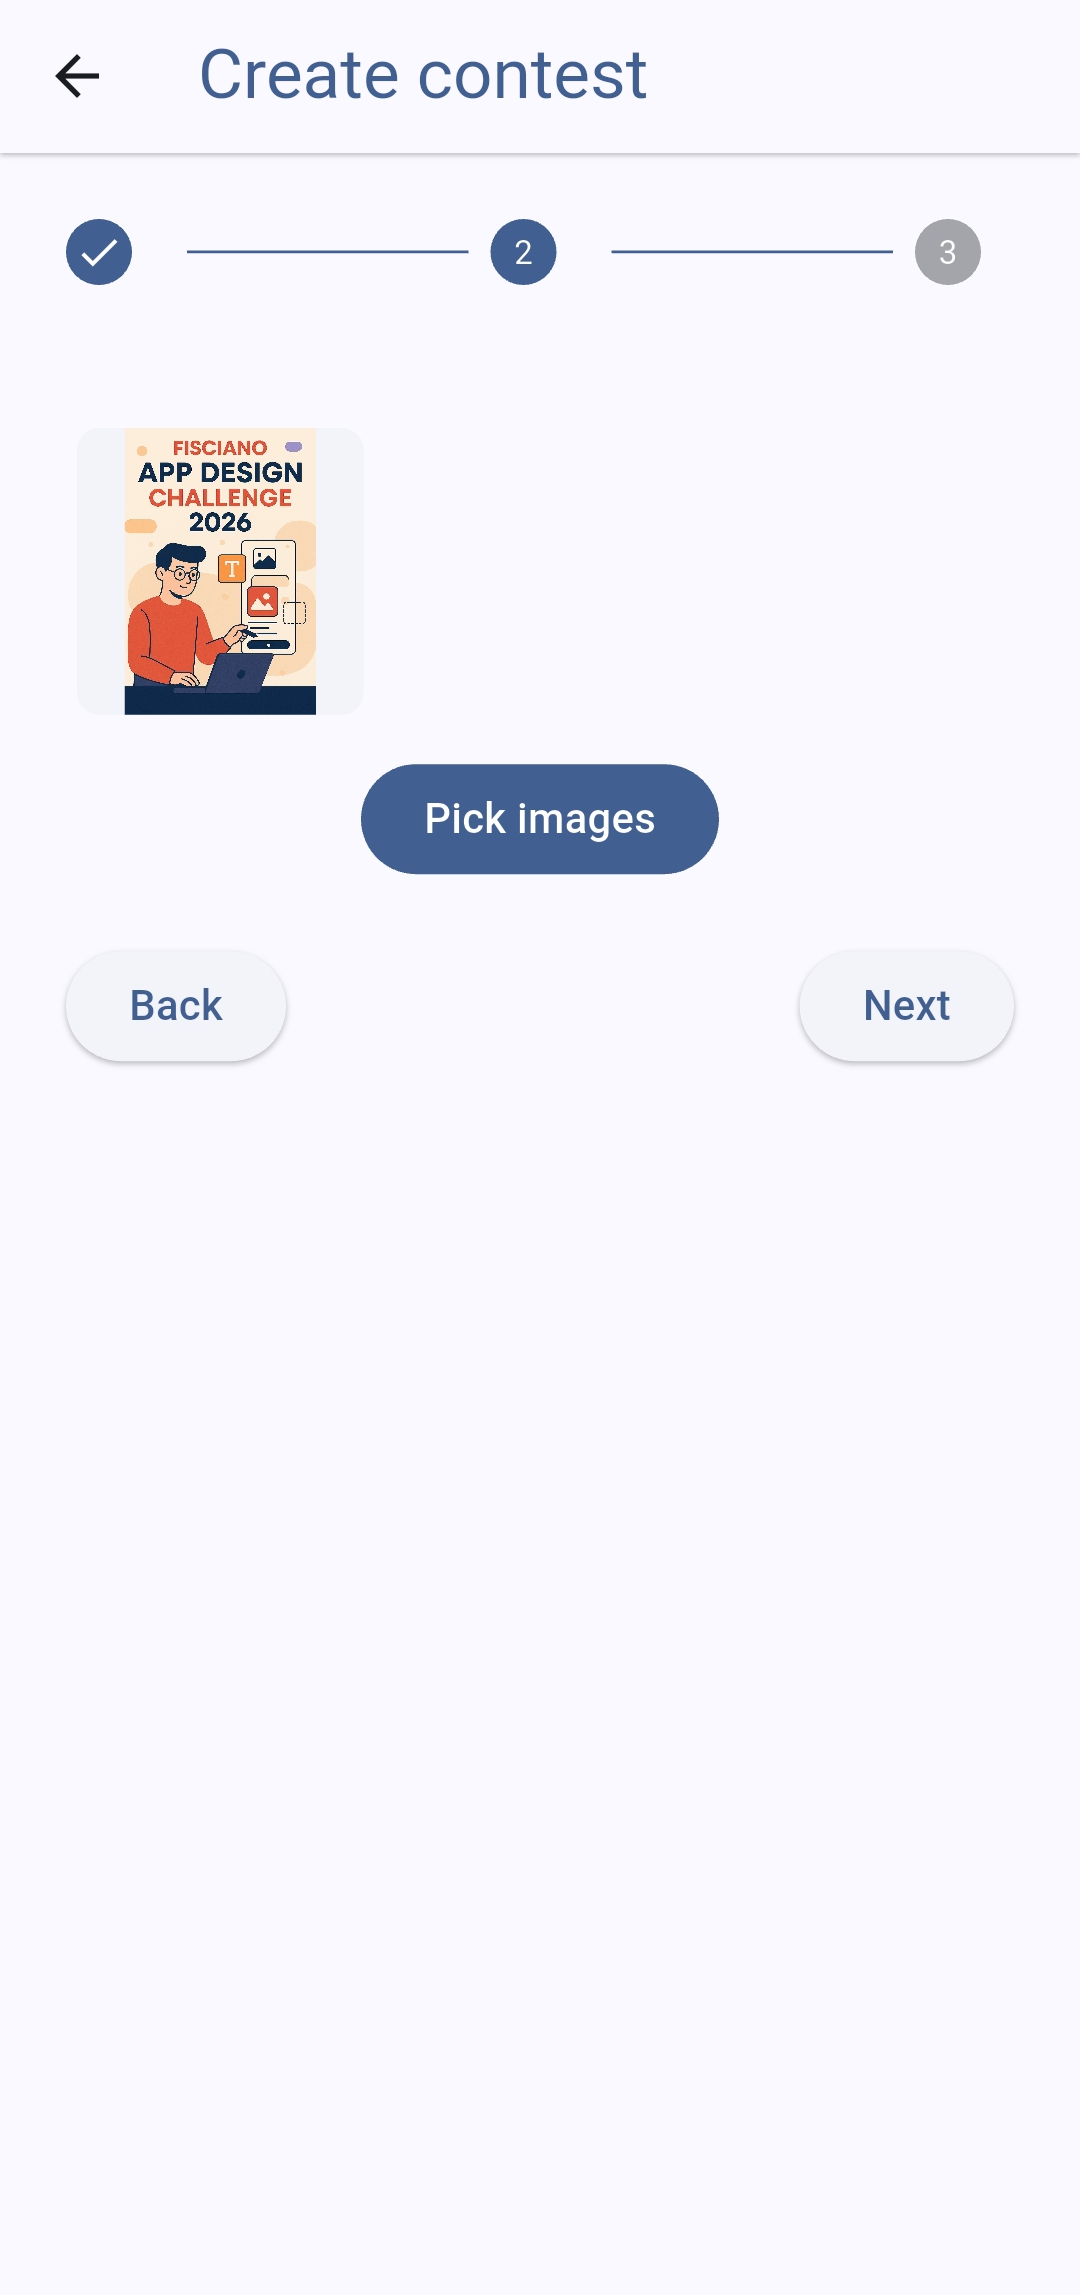
\includegraphics[width=\linewidth]{figure/organizer-create-contest-step2}
        \subcaption{Passo 2: Immagini}
        \label{fig:create_contest_2}
    \end{minipage}\hfill
    \begin{minipage}[t]{0.30\textwidth}
        \centering
        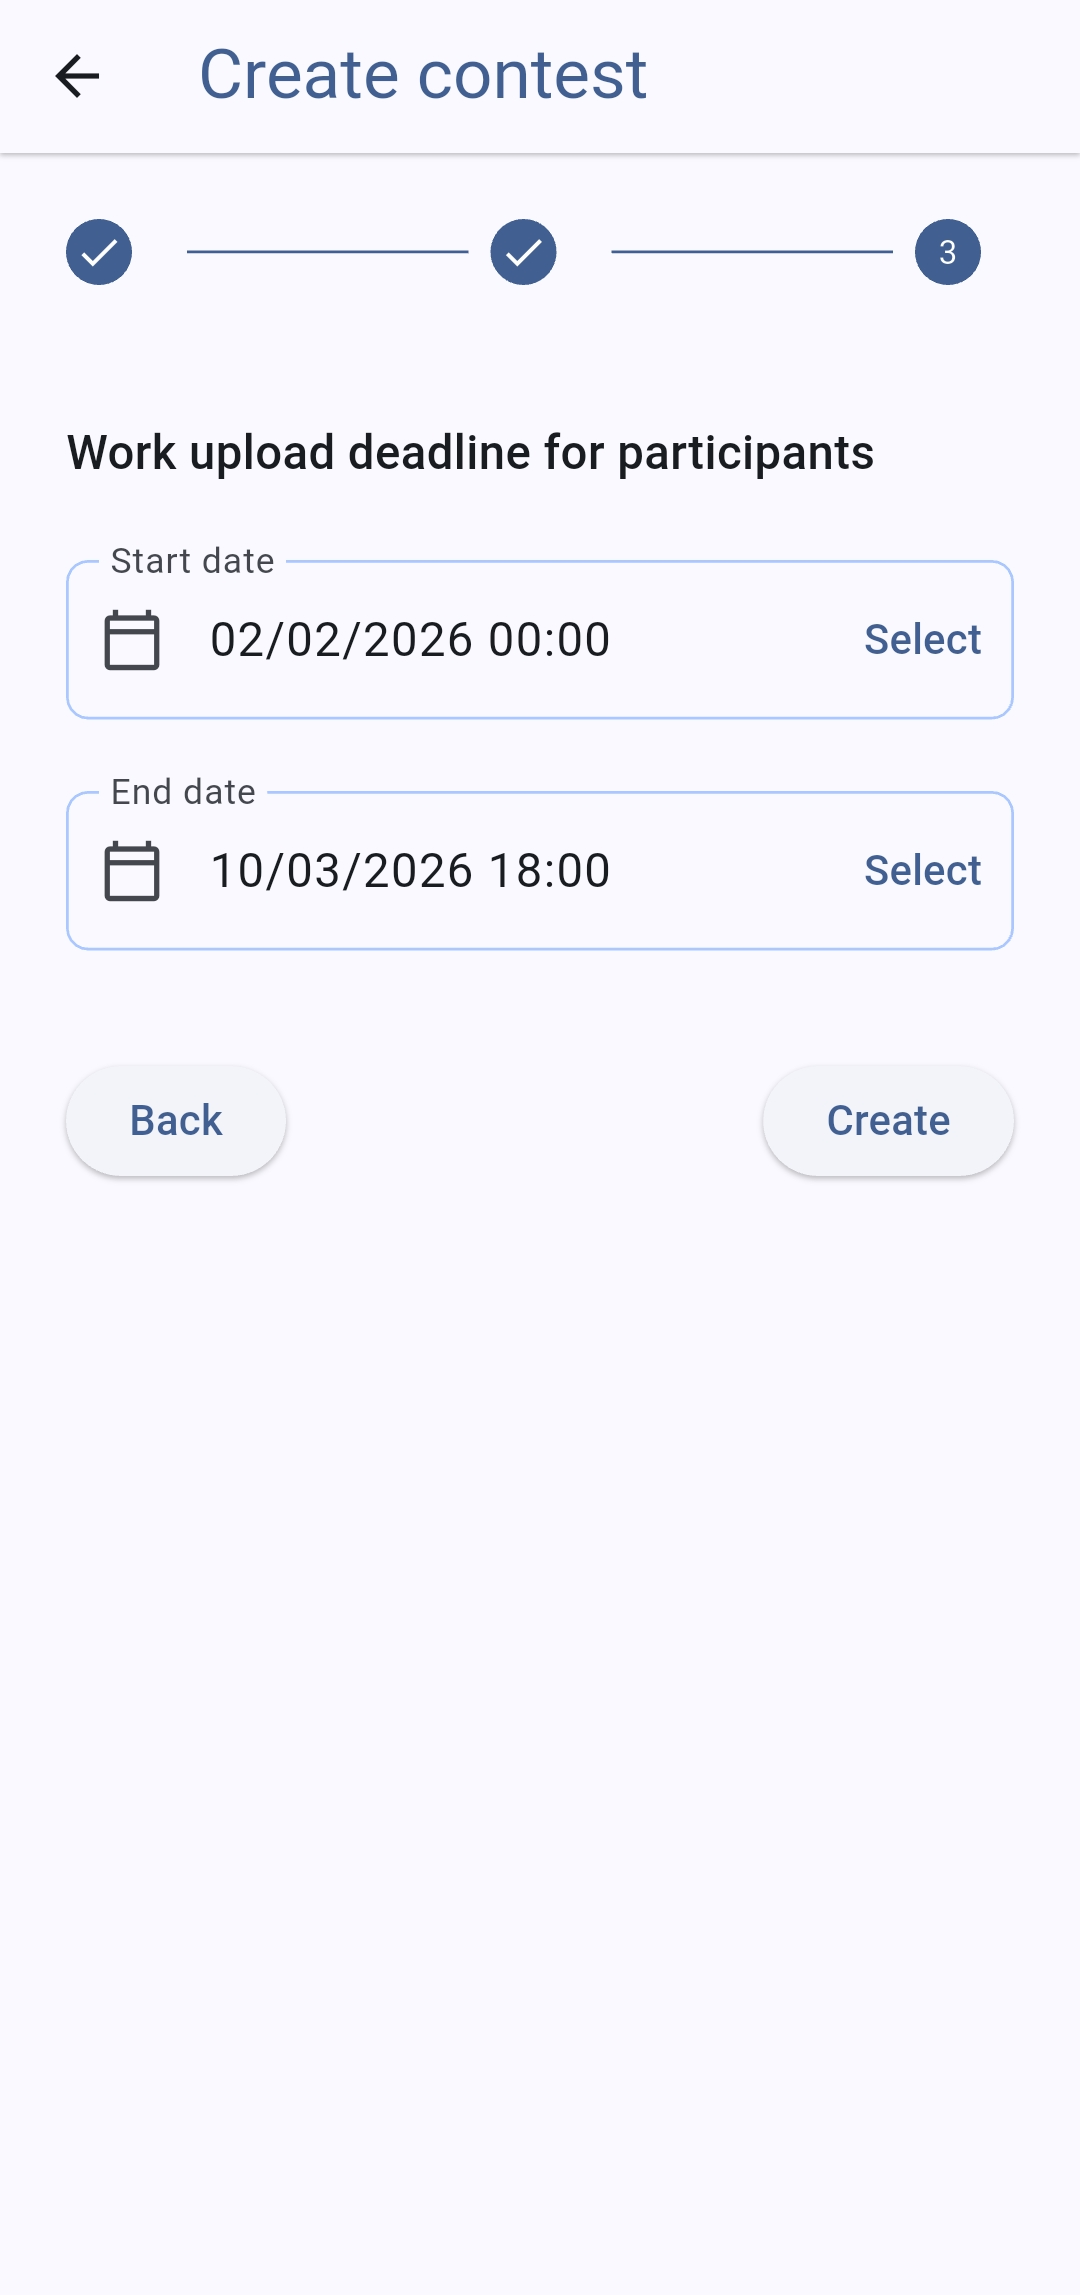
\includegraphics[width=\linewidth]{figure/organizer-create-contest-step3}
        \subcaption{Passo 3: Periodo sottomissione}
        \label{fig:create_contest_3}
    \end{minipage}
    \caption{Le tre schermate del form guidato per la creazione di un nuovo contest.}
    \label{fig:create_contest_flow}
\end{figure}

\paragraph{Configurazione dei Dettagli del Contest}
Selezionando un contest dalla home page, l'organizzatore accede al pannello di gestione, organizzato in tab.
Da qui può configurare ogni aspetto del contest:
\begin{itemize}
    \item La tab \textbf{Details} funge da pagina di riepilogo, mostrando tutte le informazioni generali del contest.
    Le azioni di modifica o cancellazione sono accessibili da un menu separato.
    \item La tab \textbf{Participants} mostra l'elenco dei partecipanti iscritti e attesi, permettendo di invitarne di nuovi.
    \item La tab \textbf{Juries} consente di creare e gestire le giurie e di configurare il \textbf{Voting Form} associato a ciascuna, definendone i campi.
    \item La tab \textbf{Works} mostra l'elenco dei lavori sottomessi dai partecipanti.
\end{itemize}

\begin{figure}[H]
    \centering
    \begin{minipage}[t]{0.30\textwidth}
        \centering
        
\includegraphics[width=\linewidth]{figure/organizer-contest-details}
        \subcaption{Tab Details}
        \label{fig:contest_details}
    \end{minipage}
    \quad
    \begin{minipage}[t]{0.30\textwidth}
        \centering
        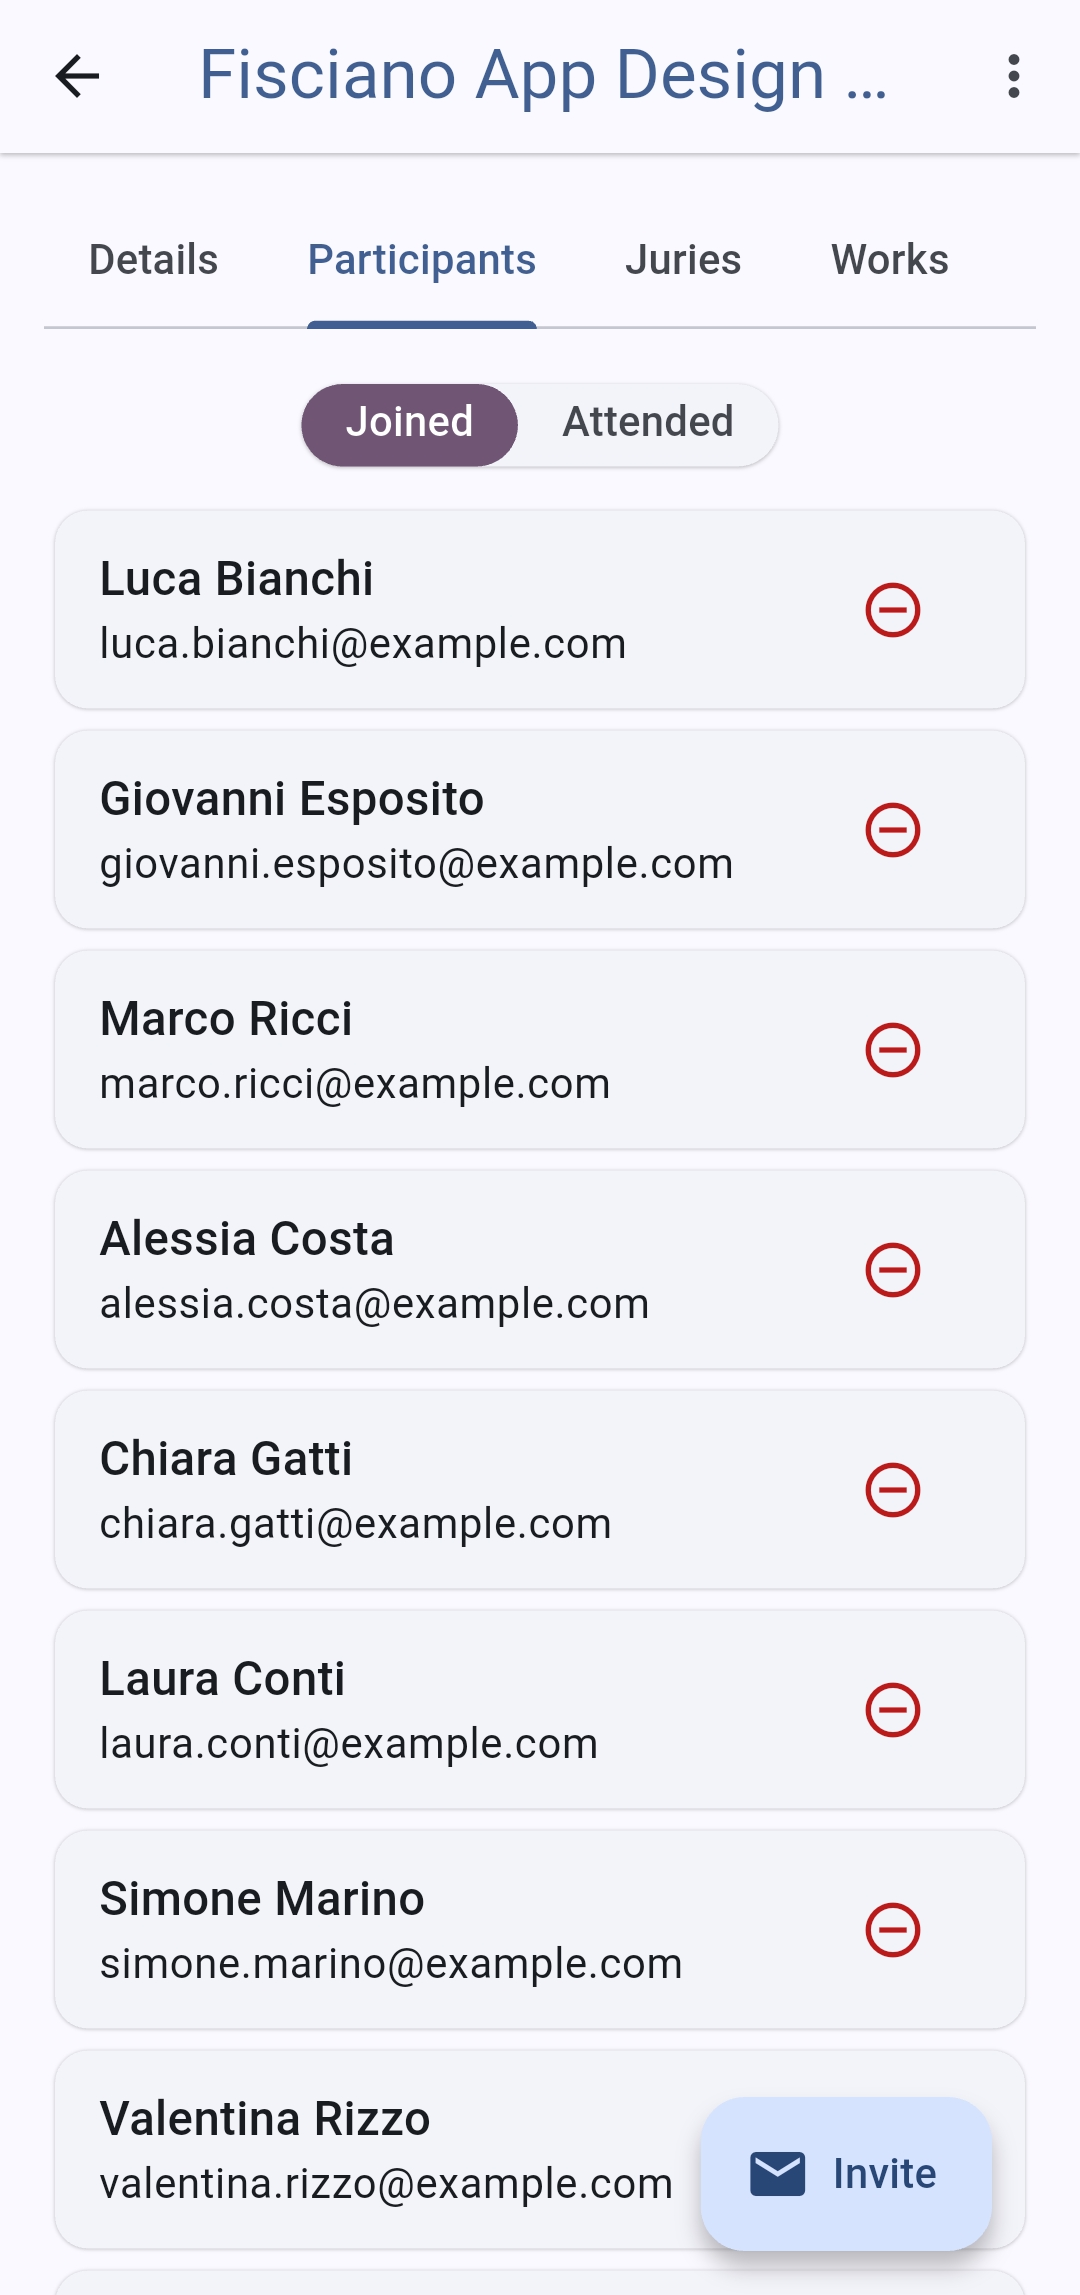
\includegraphics[width=\linewidth]{figure/organizer-contest-participants}
        \subcaption{Tab Participants}
        \label{fig:contest_participants}
    \end{minipage}

    \vspace{1em} % Spazio tra le righe di immagini

    \begin{minipage}[t]{0.30\textwidth}
        \centering
        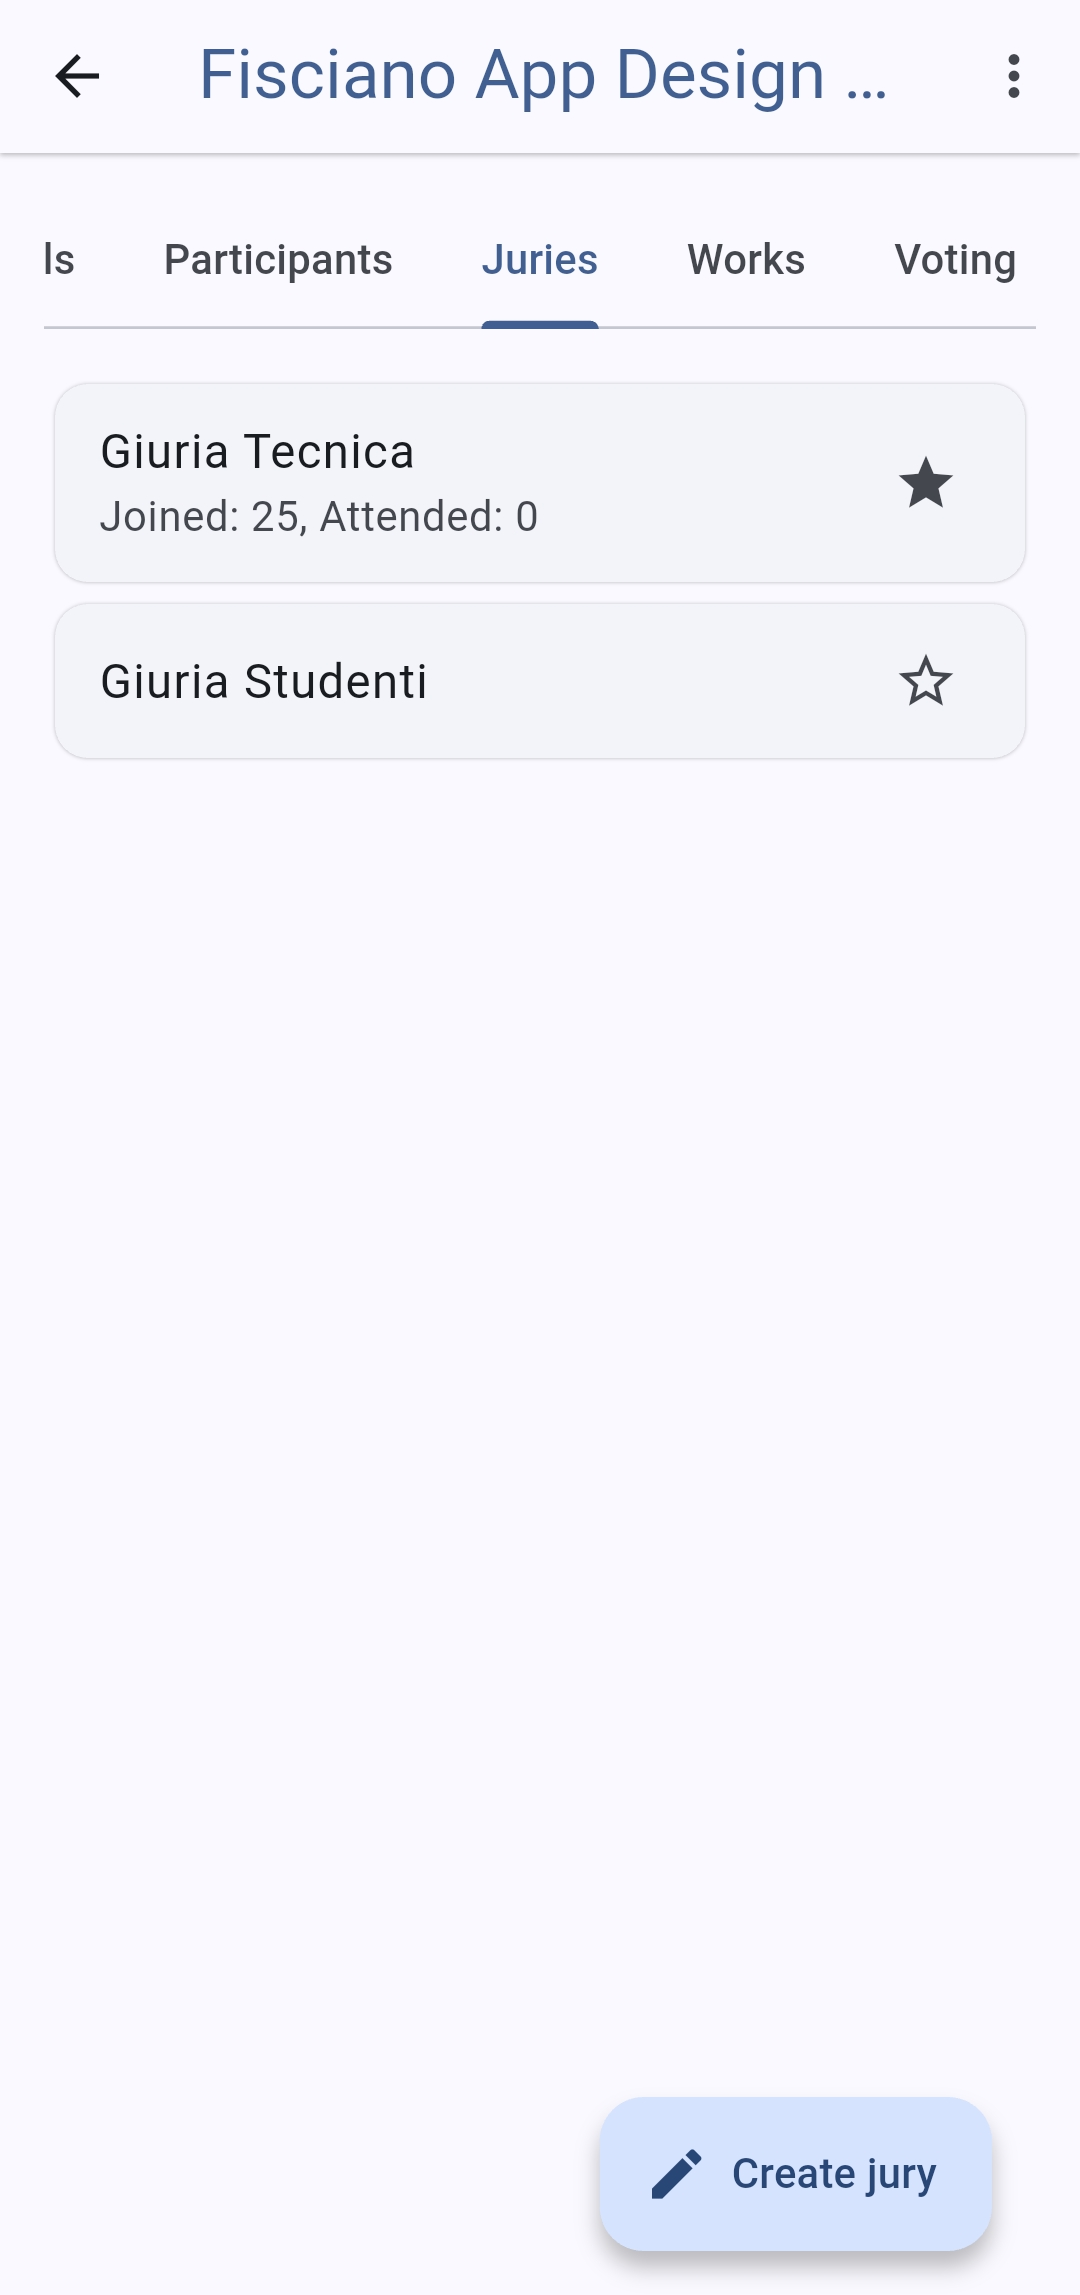
\includegraphics[width=\linewidth]{figure/organizer-contest-juries}
        \subcaption{Tab Juries}
        \label{fig:contest_juries}
    \end{minipage}
    \quad
    \begin{minipage}[t]{0.30\textwidth}
        \centering
        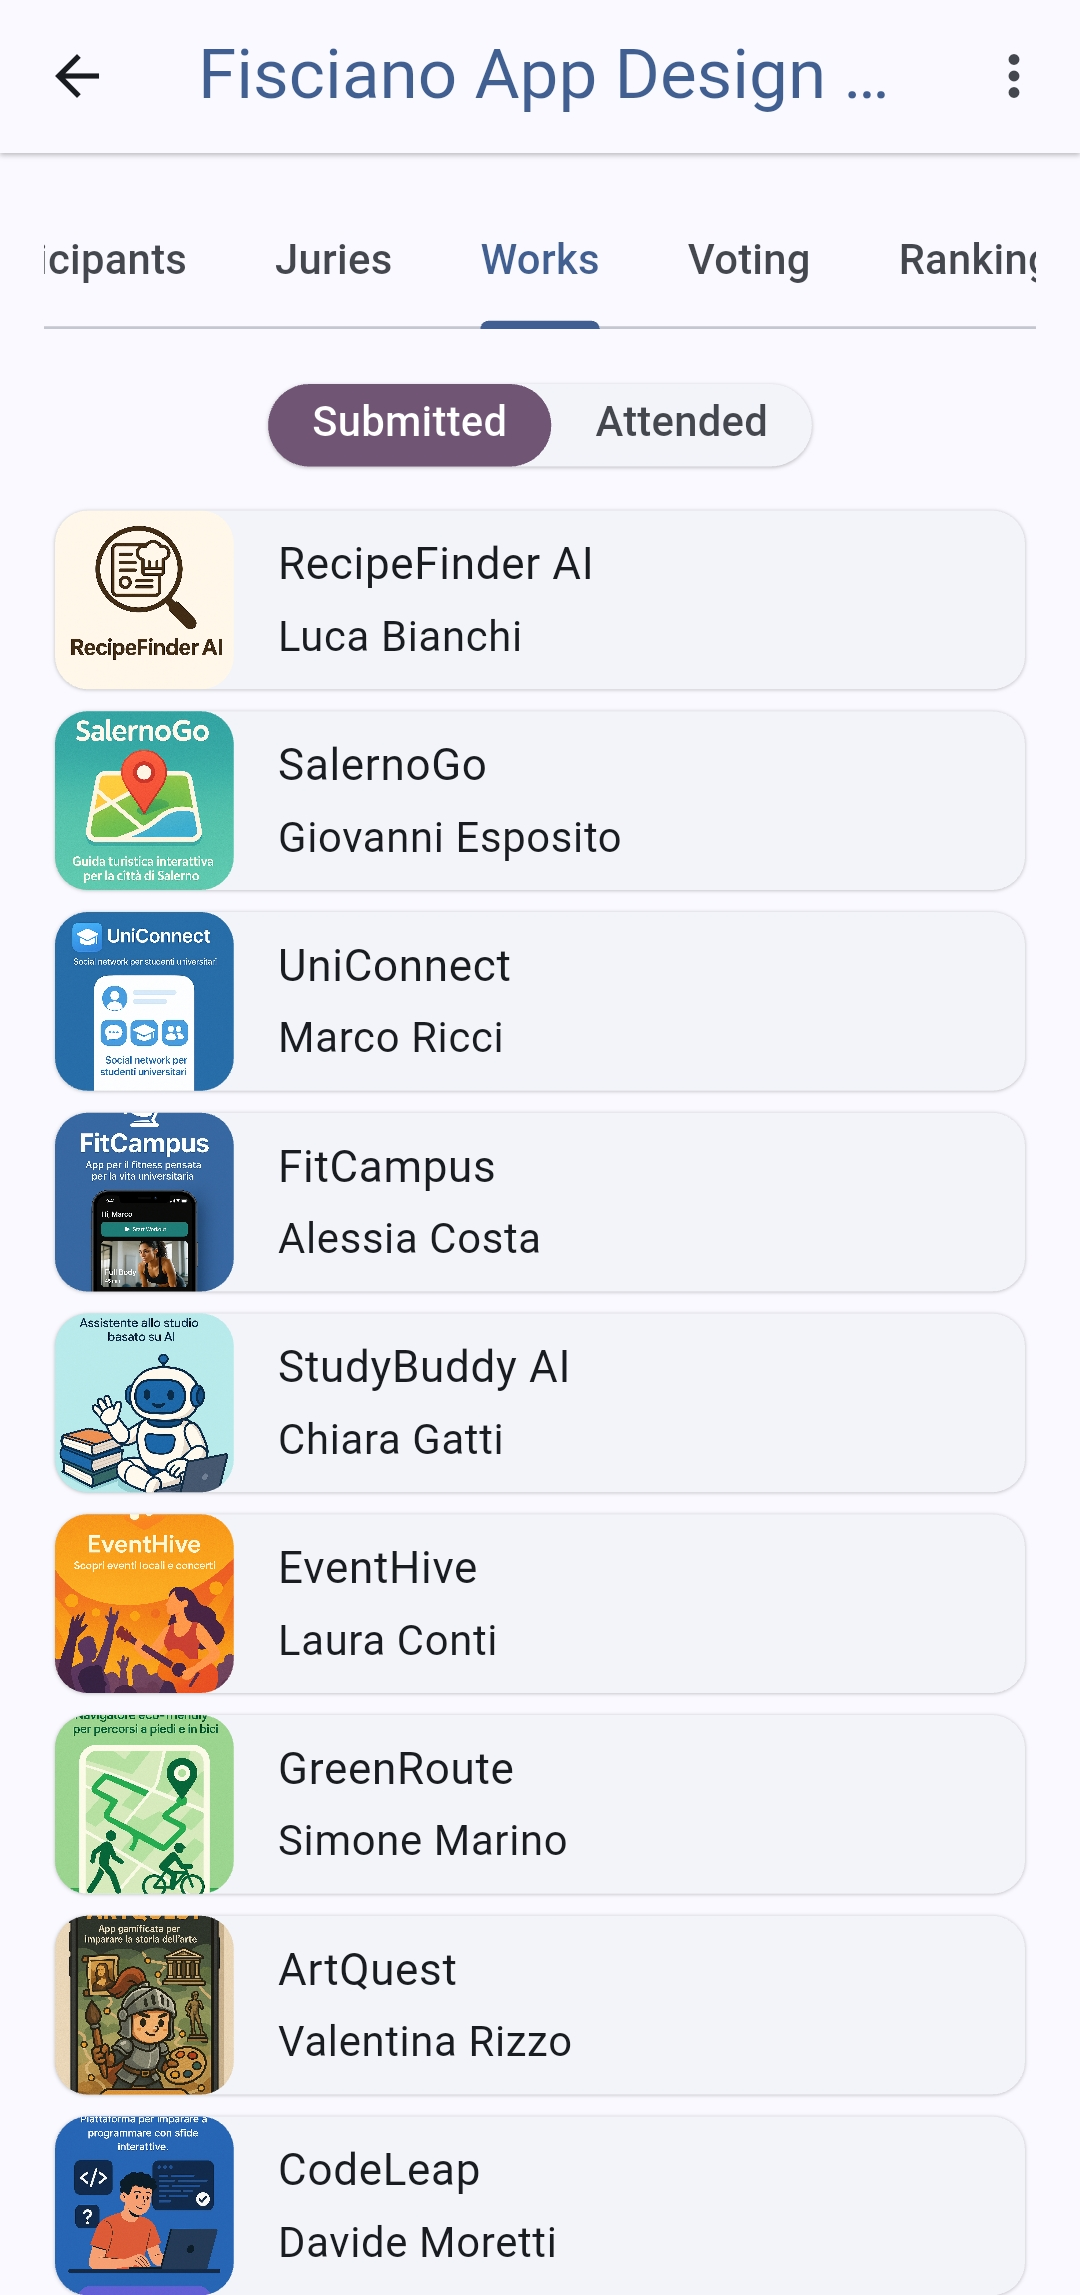
\includegraphics[width=\linewidth]{figure/organizer-contest-works}
        \subcaption{Tab Works}
        \label{fig:contest_works}
    \end{minipage}
    \caption{Le principali tab di gestione all'interno di un contest.}
    \label{fig:contest_management_tabs}
\end{figure}

In particolare, la gestione delle giurie prevede una schermata di dettaglio il cui contenuto \textbf{varia a seconda del tipo di giuria}.
Questa scelta di design permette di presentare all'organizzatore solo le informazioni e le azioni pertinenti:
\begin{itemize}
    \item Per una \textbf{giuria nominata (\emph{appointed})}, la pagina mostra l'elenco dei giurati iscritti e invitati.
    \item Per una \textbf{giuria semplice (\emph{simple})}, la pagina non mostra un elenco di utenti, ma espone il \textbf{token} di accesso che l'organizzatore può condividere.
\end{itemize}
Per entrambe, è possibile accedere alla configurazione del \textbf{Voting Form} associato.

% --- FIGURE: Dettaglio Giuria e Configurazione Form ---
\begin{figure}[H]
    \centering
    \begin{minipage}[t]{0.30\textwidth}
        \centering
        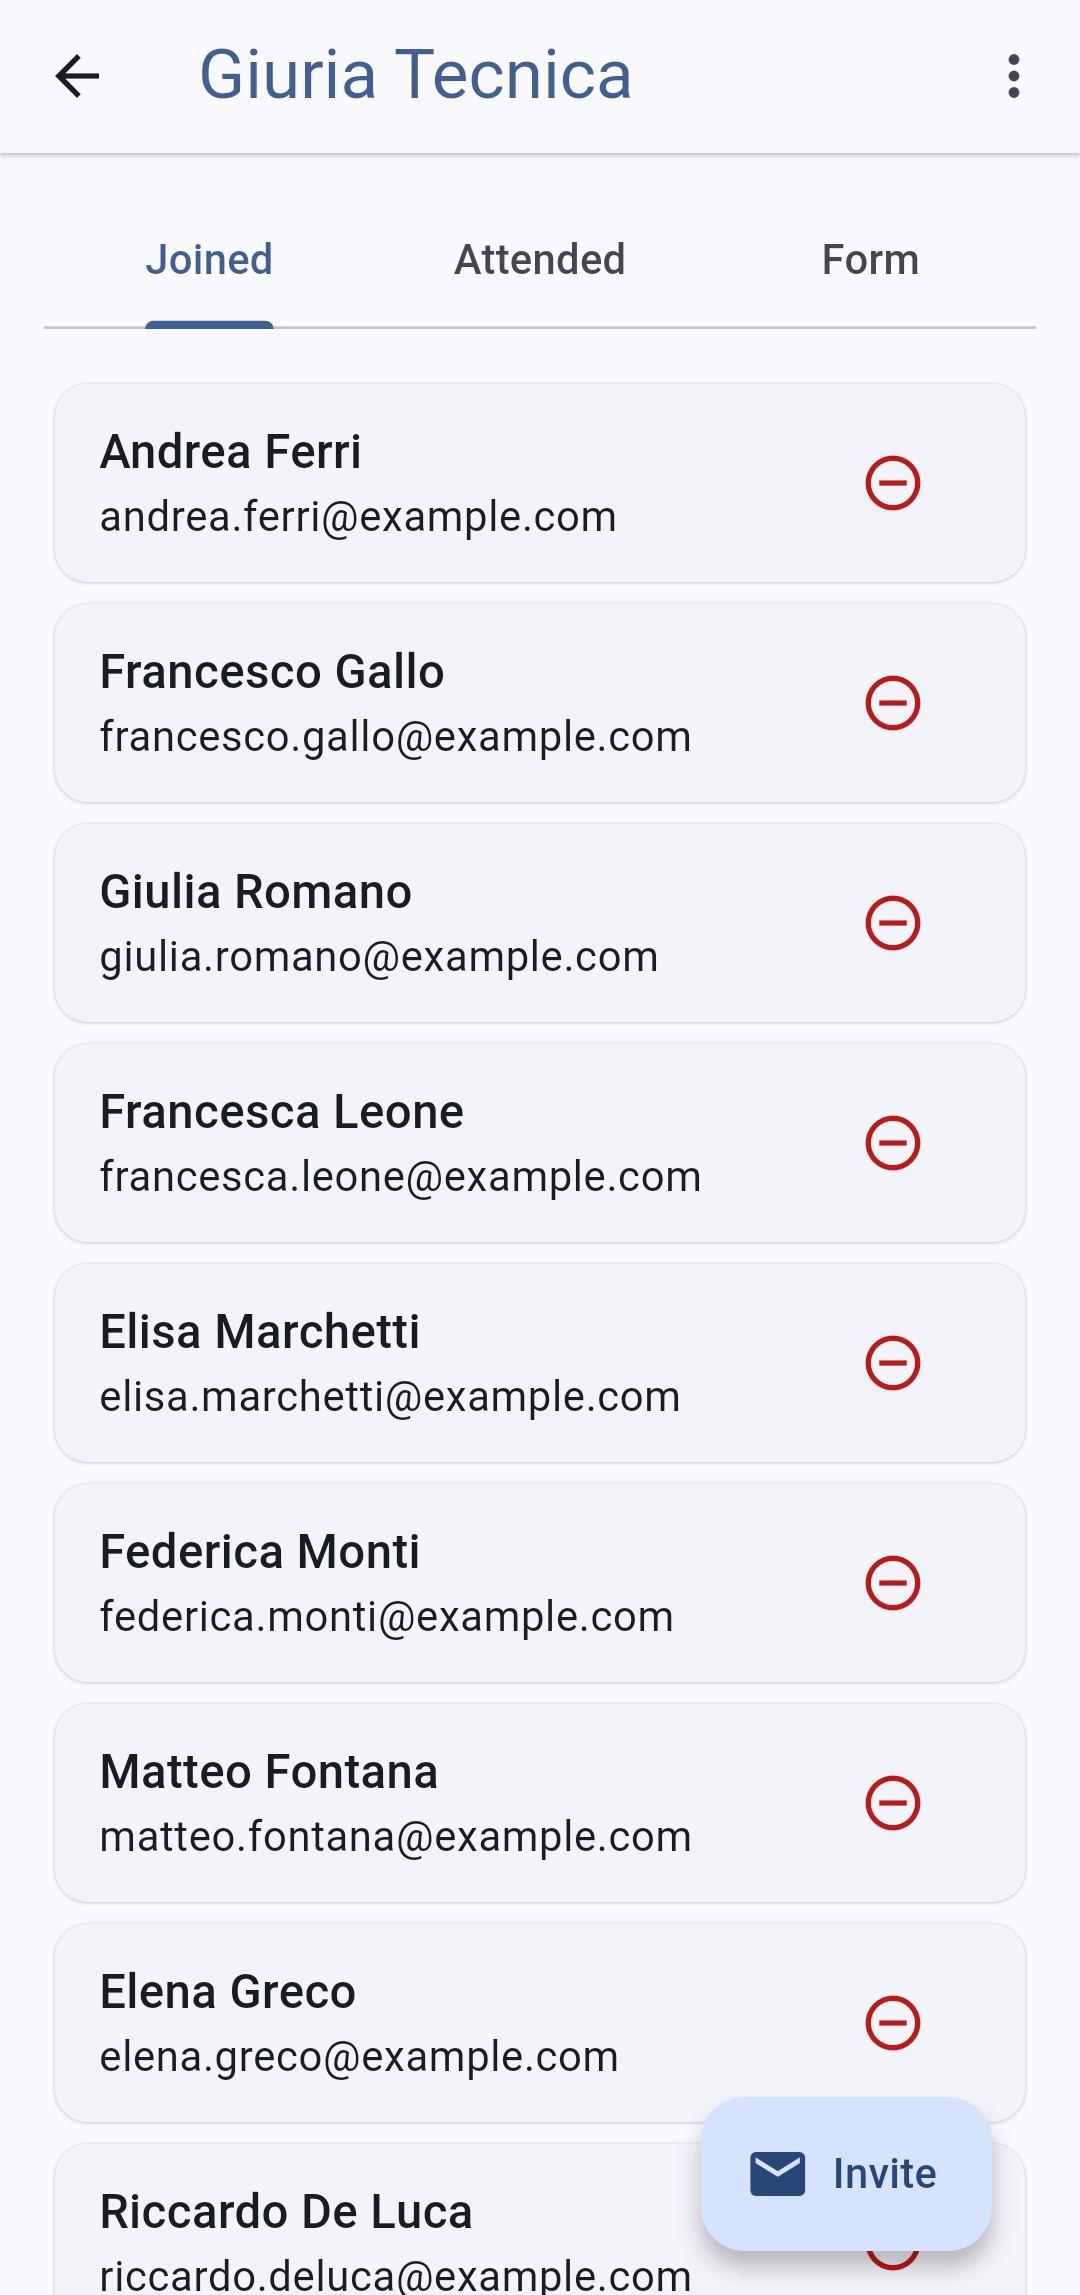
\includegraphics[width=\linewidth]{figure/organizer-appointed-jury}
        \subcaption{Dettaglio Giuria Nominata}
        \label{fig:jury_details_appointed}
    \end{minipage}\hfill
    \begin{minipage}[t]{0.30\textwidth}
        \centering
        
\includegraphics[width=\linewidth]{figure/organizer-jury-voting-form}
        \subcaption{Configurazione Voting Form}
        \label{fig:voting_form_edit}
    \end{minipage}\hfill
    \begin{minipage}[t]{0.30\textwidth}
        \centering
        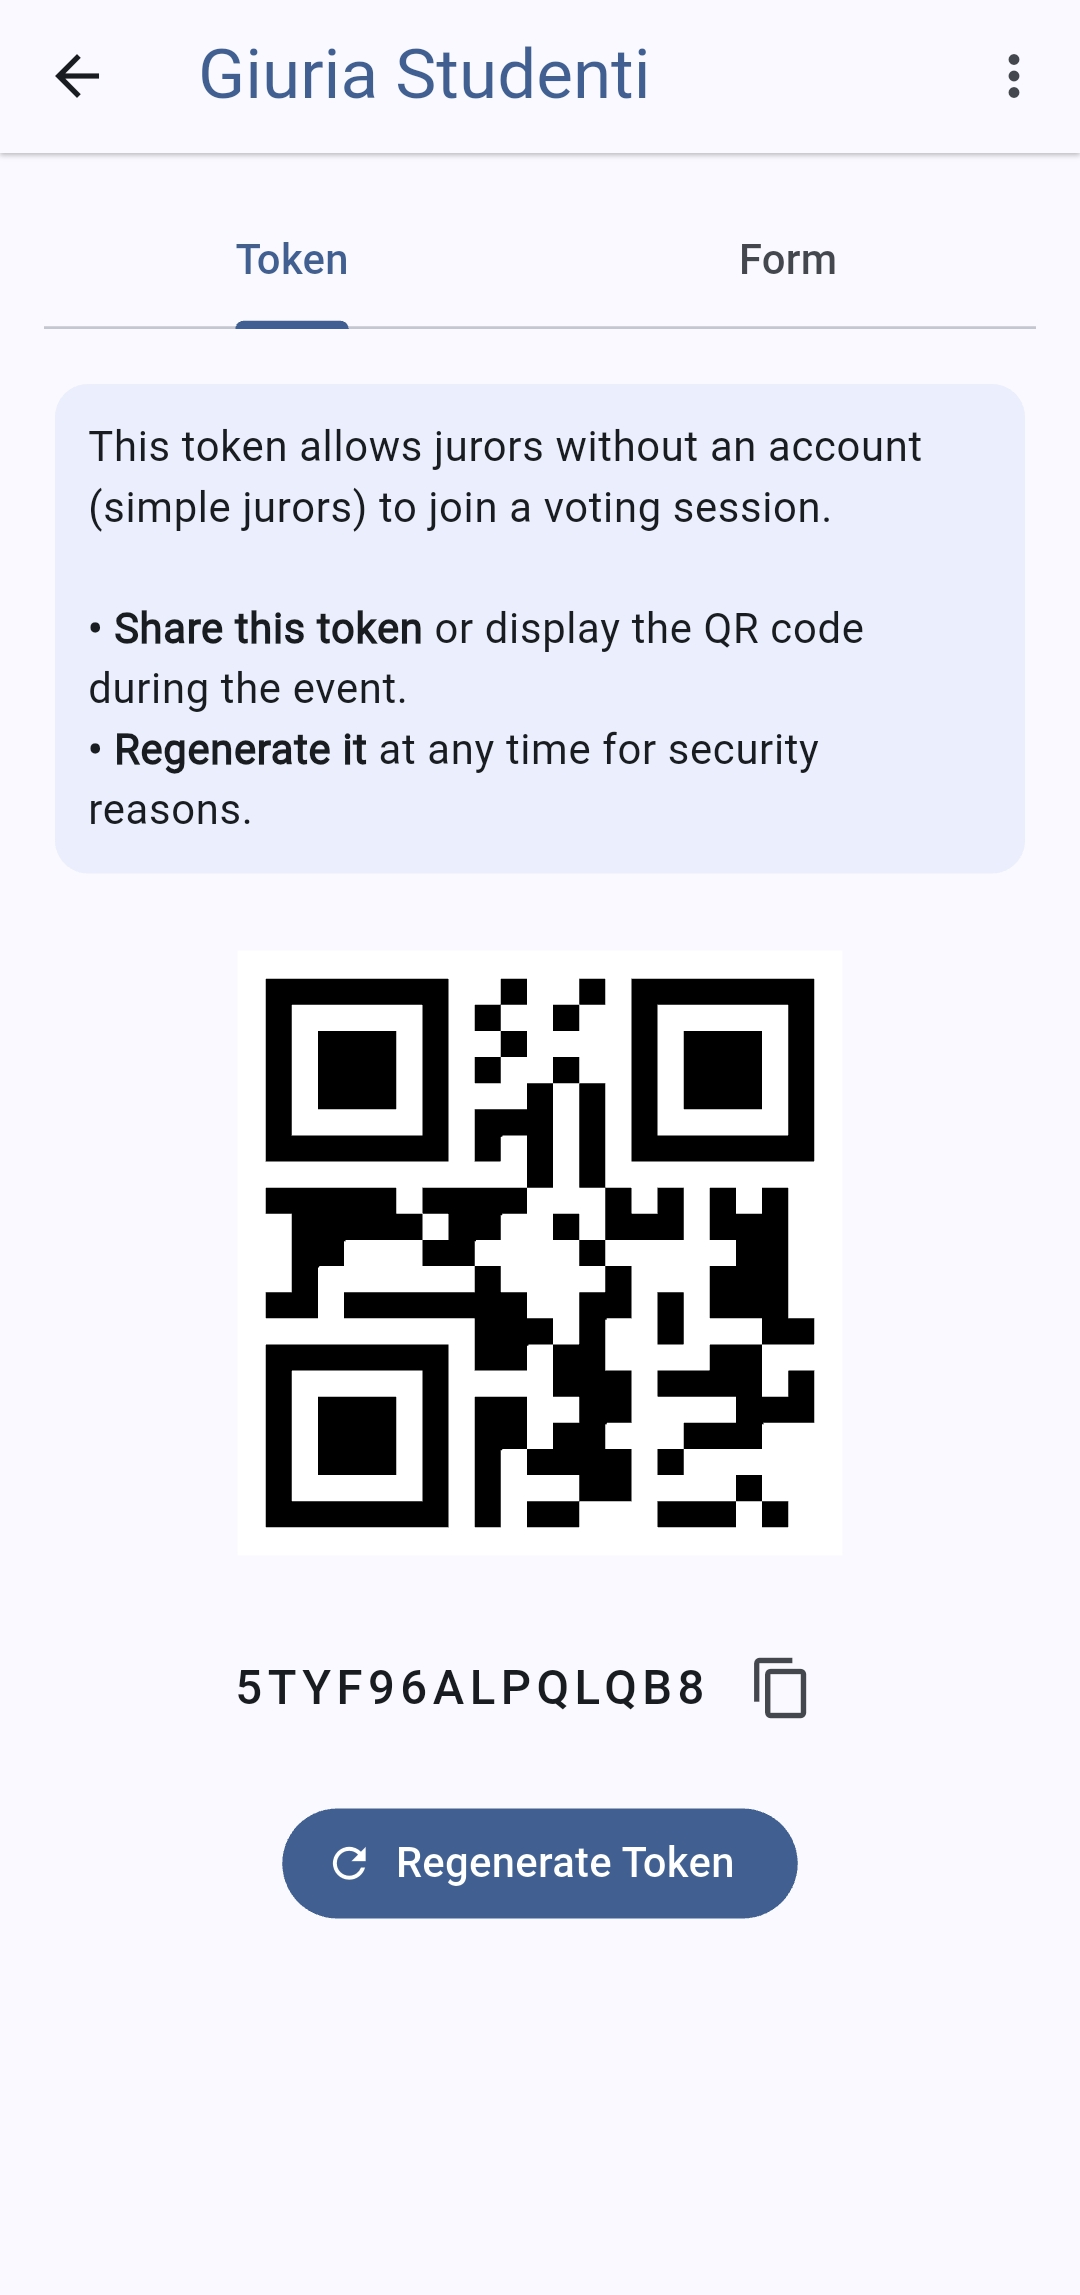
\includegraphics[width=\linewidth]{figure/organizer-simple-jury}
        \subcaption{Dettaglio Giuria Semplice}
        \label{fig:jury_details_simple}
    \end{minipage}
    \caption{Le viste di dettaglio per i due tipi di giuria e la schermata di configurazione del \emph{Voting Form} associato.}
    \label{fig:jury_and_form_views}
\end{figure}

\paragraph{Gestione della Sessione di Voto}
La tab \textbf{Voting} è dedicata alla gestione delle sessioni di voto.
Da qui, l'organizzatore può avviare una nuova sessione tramite un form a tre passaggi, che gli permette di configurare con precisione l'ambiente di votazione:
\begin{enumerate}
    \item \textbf{Selezione dei Partecipanti}: scelta dei partecipanti da includere nella sessione di voto.
    \item \textbf{Geo-restrizione}: impostazione opzionale di una restrizione geografica, che obbliga i giurati a votare solo se si trovano entro un certo raggio dal luogo del contest.
    \item \textbf{Gestione Esclusioni}: revisione e applicazione delle regole di esclusione, che impediscono a specifici giurati di votare per determinati partecipanti.
\end{enumerate}
Una volta avviata, la schermata mostra lo stato \textbf{Live} della sessione, il token per i giurati semplici e permette di monitorarne l'andamento.

% --- FIGURE: Avvio Sessione di Voto (3+1 immagini) ---
\begin{figure}[H]
    \centering
    \begin{minipage}[t]{0.30\textwidth}
        \centering
        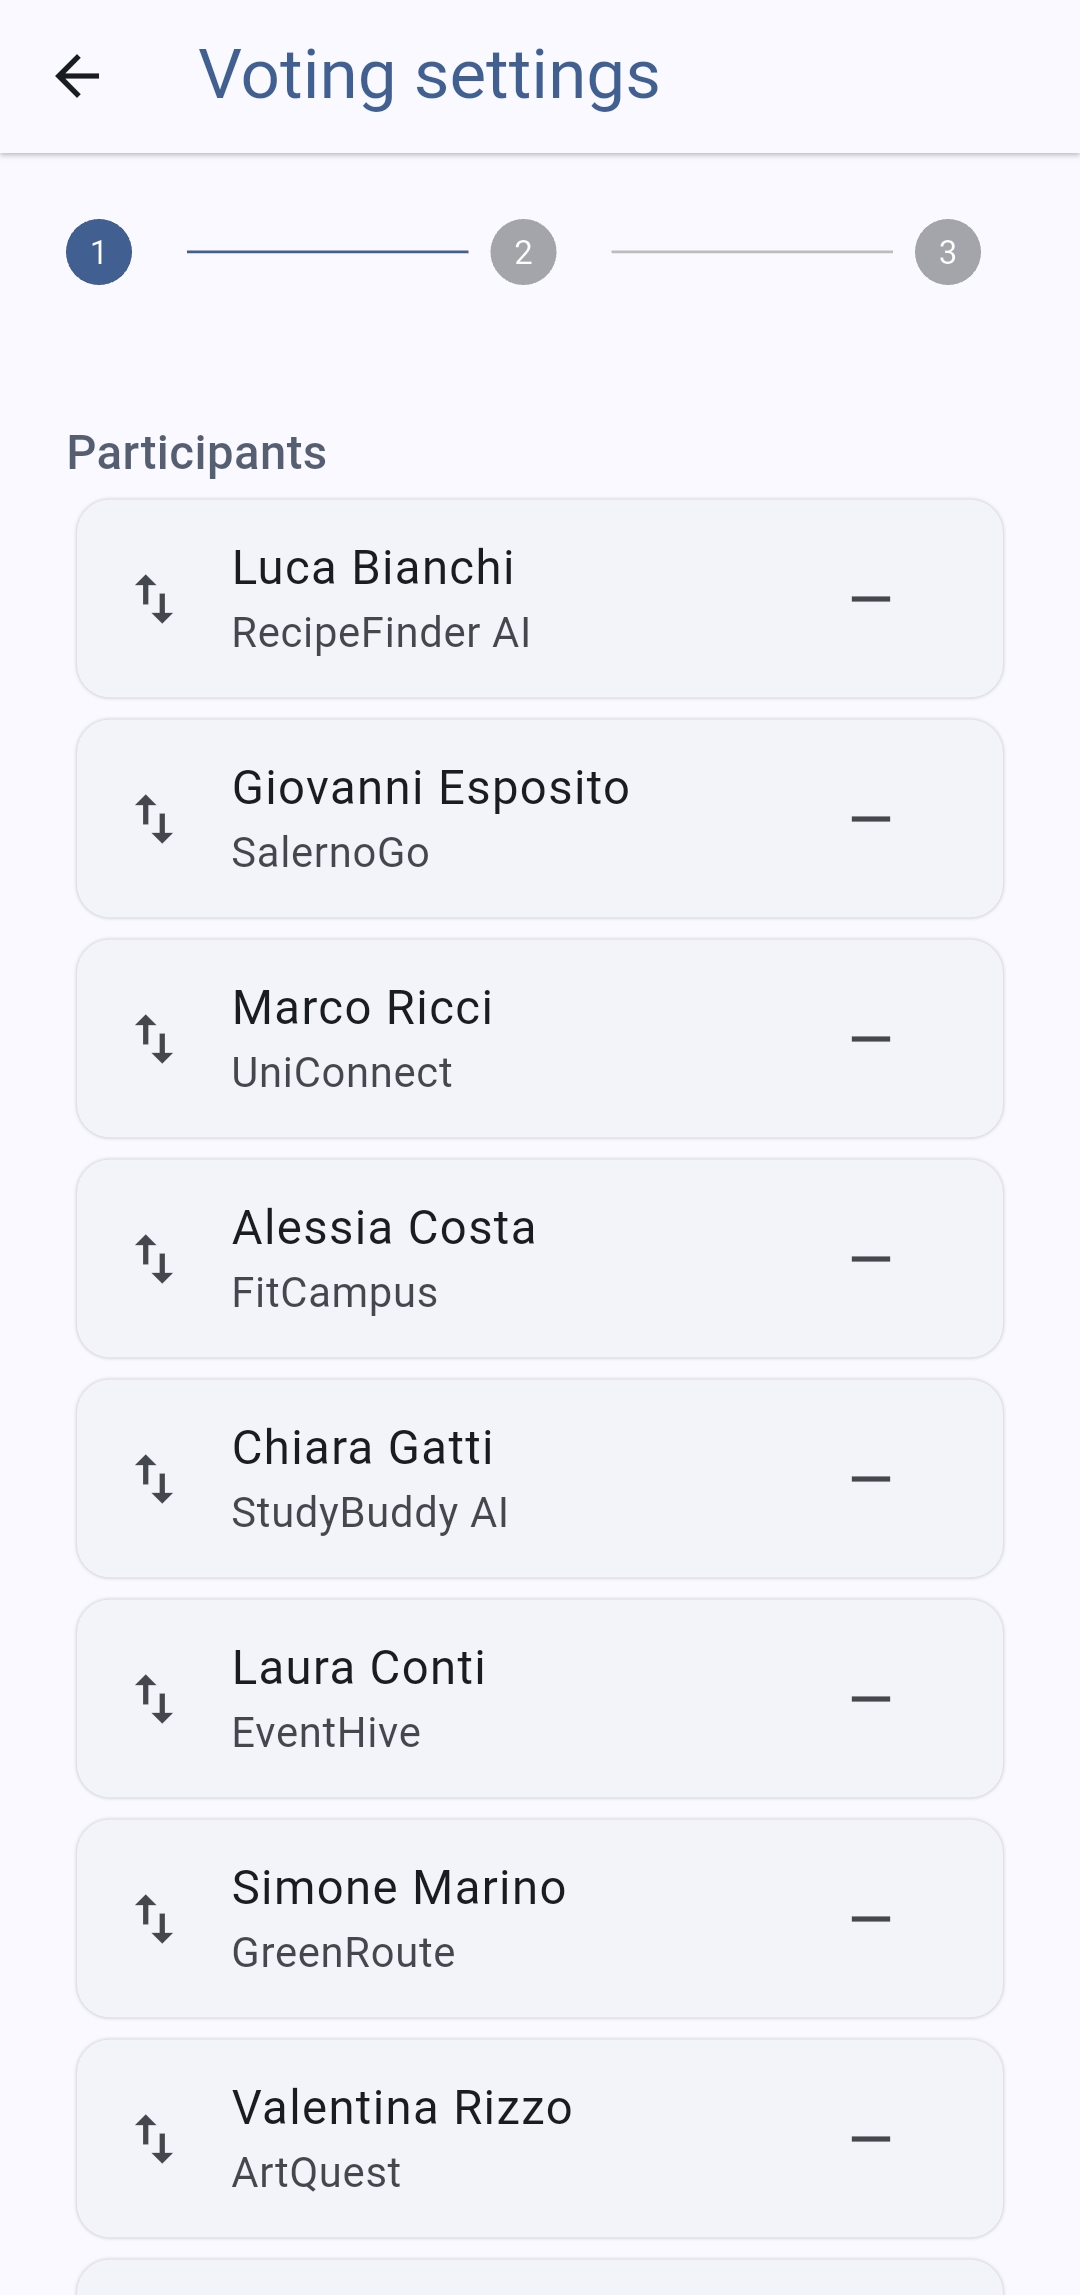
\includegraphics[width=\linewidth]{figure/organizer-voting-session-step1}
        \subcaption{Passo 1: Partecipanti}
        \label{fig:voting_session_1}
    \end{minipage}\hfill
    \begin{minipage}[t]{0.30\textwidth}
        \centering
        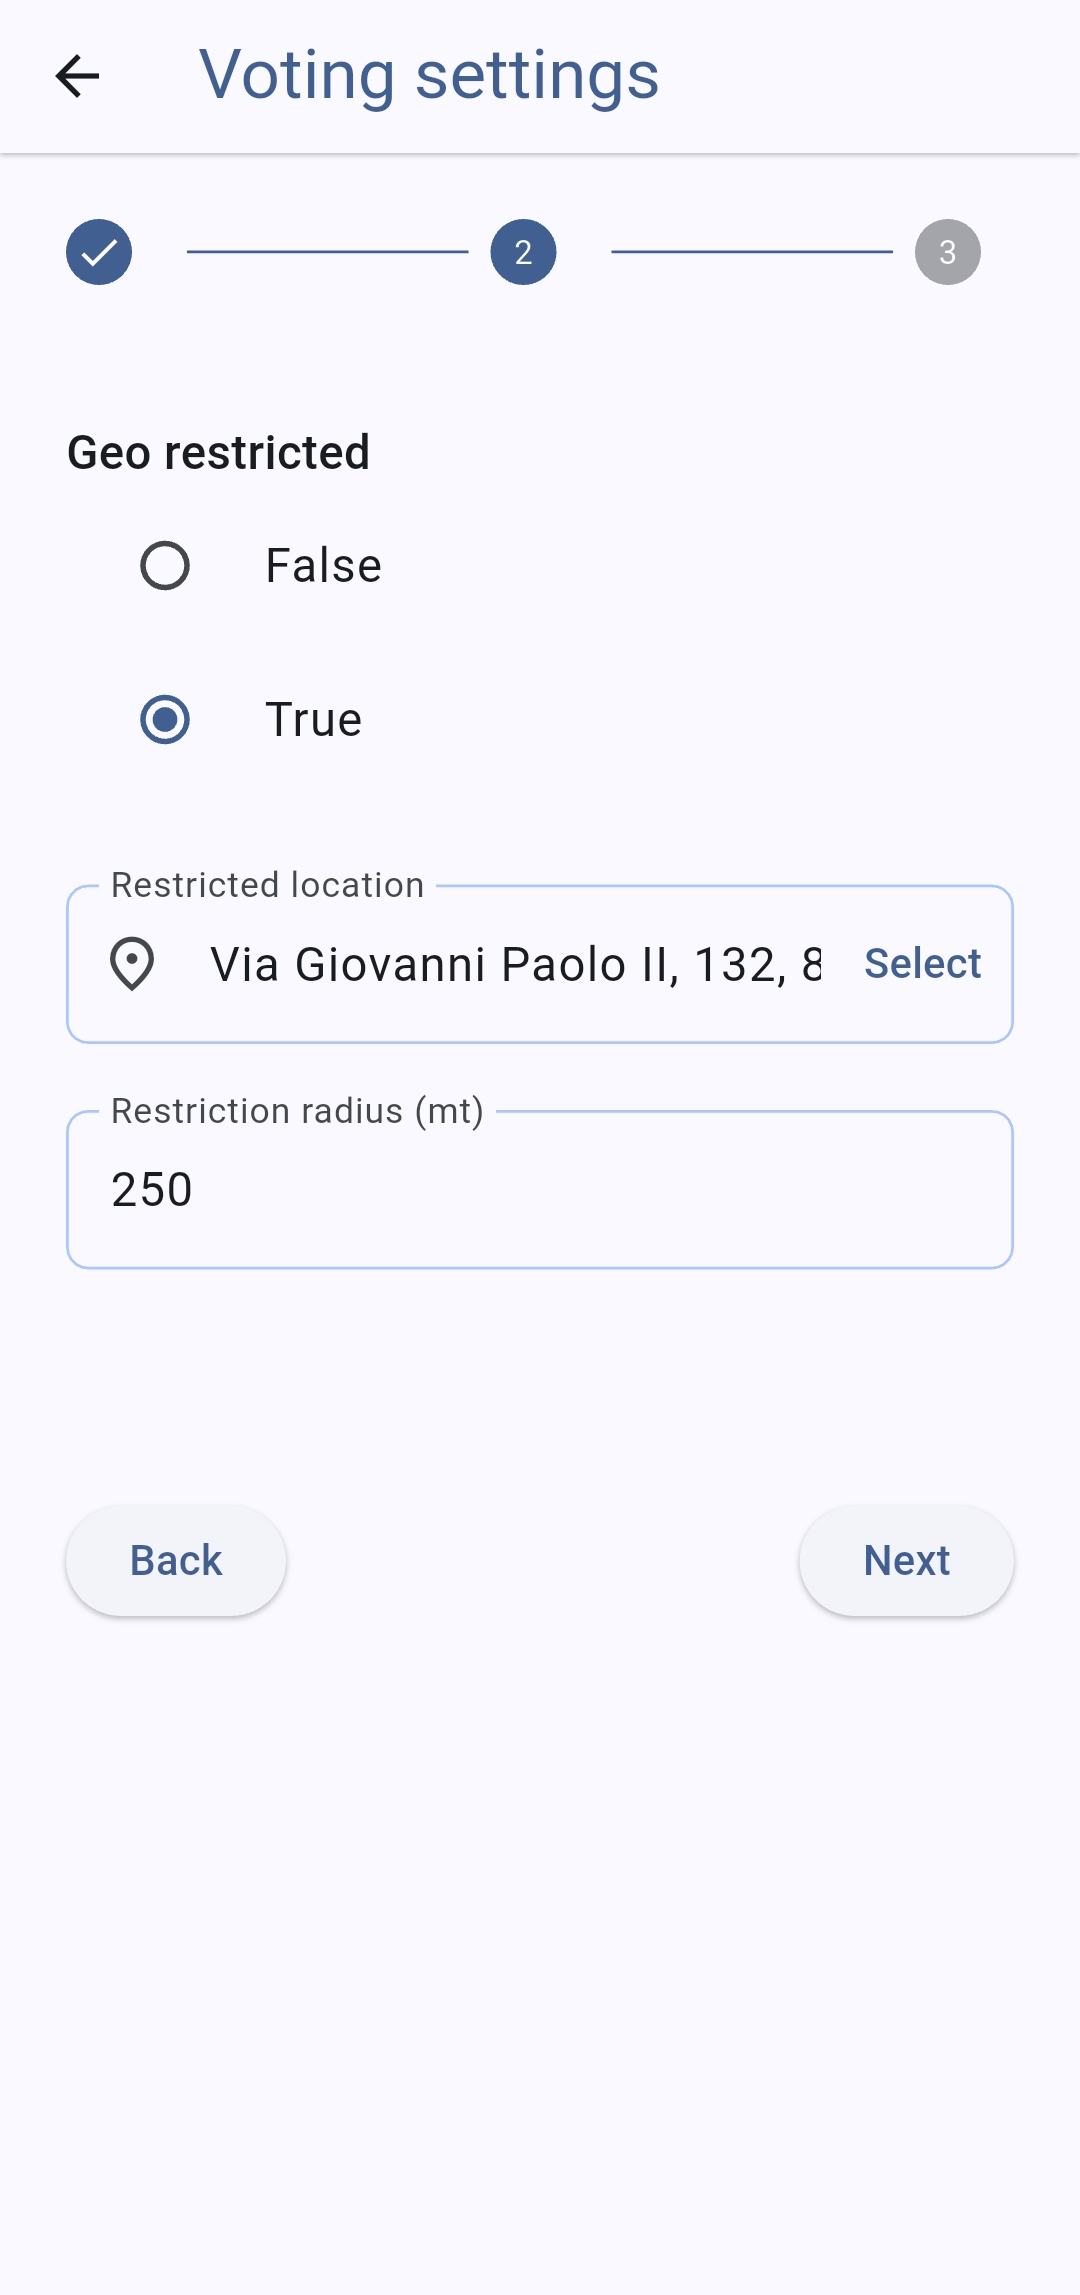
\includegraphics[width=\linewidth]{figure/organizer-voting-session-step2}
        \subcaption{Passo 2: Geo-restrizione}
        \label{fig:voting_session_2}
    \end{minipage}\hfill
    \begin{minipage}[t]{0.30\textwidth}
        \centering
        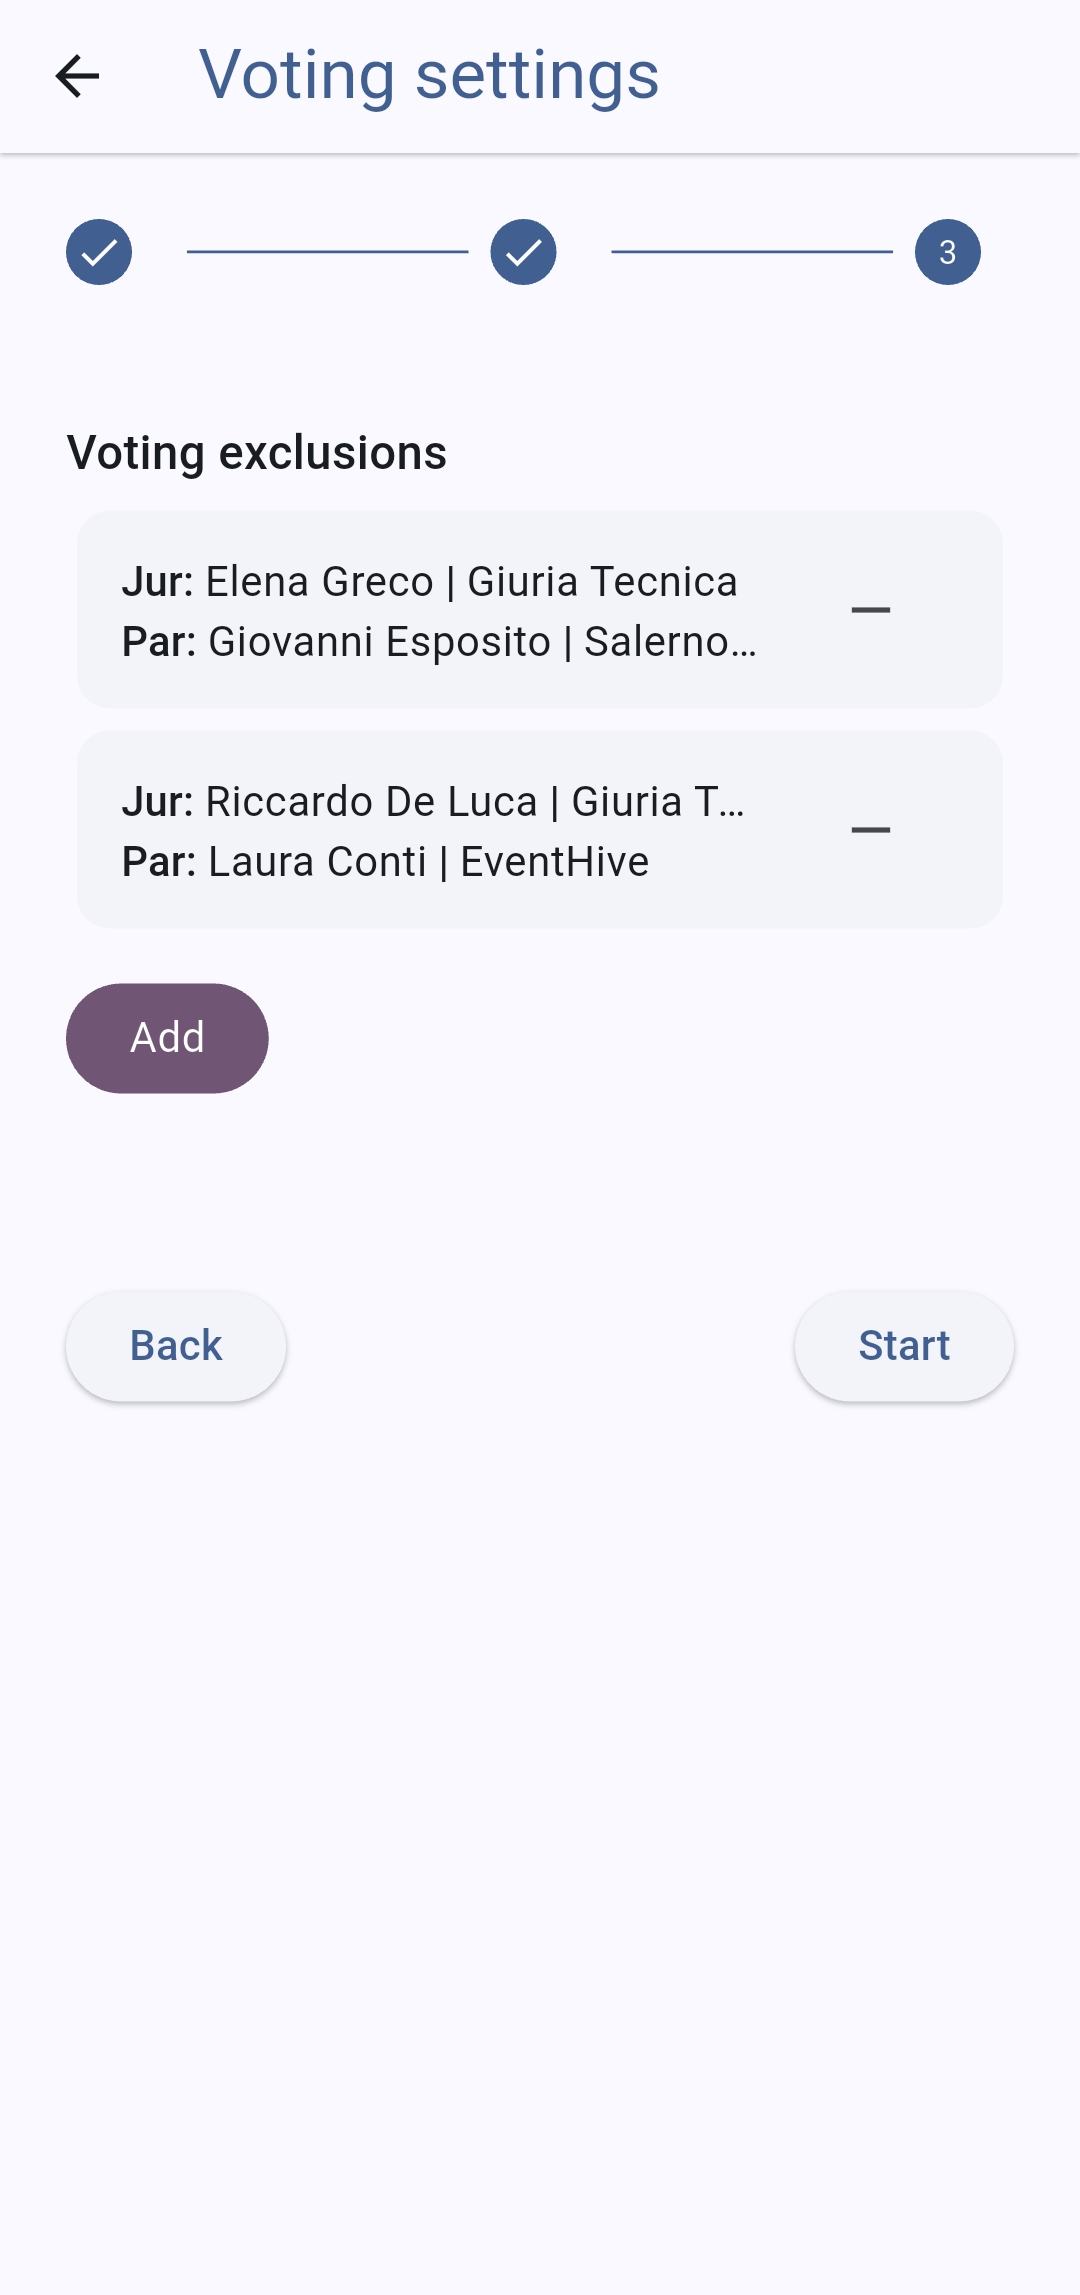
\includegraphics[width=\linewidth]{figure/organizer-voting-session-step3}
        \subcaption{Passo 3: Esclusioni}
        \label{fig:voting_session_3}
    \end{minipage}
    \caption{I passaggi per la configurazione di una nuova sessione di voto.}
    \label{fig:voting-session-setup}
\end{figure}

\begin{figure}[H]
    \centering
    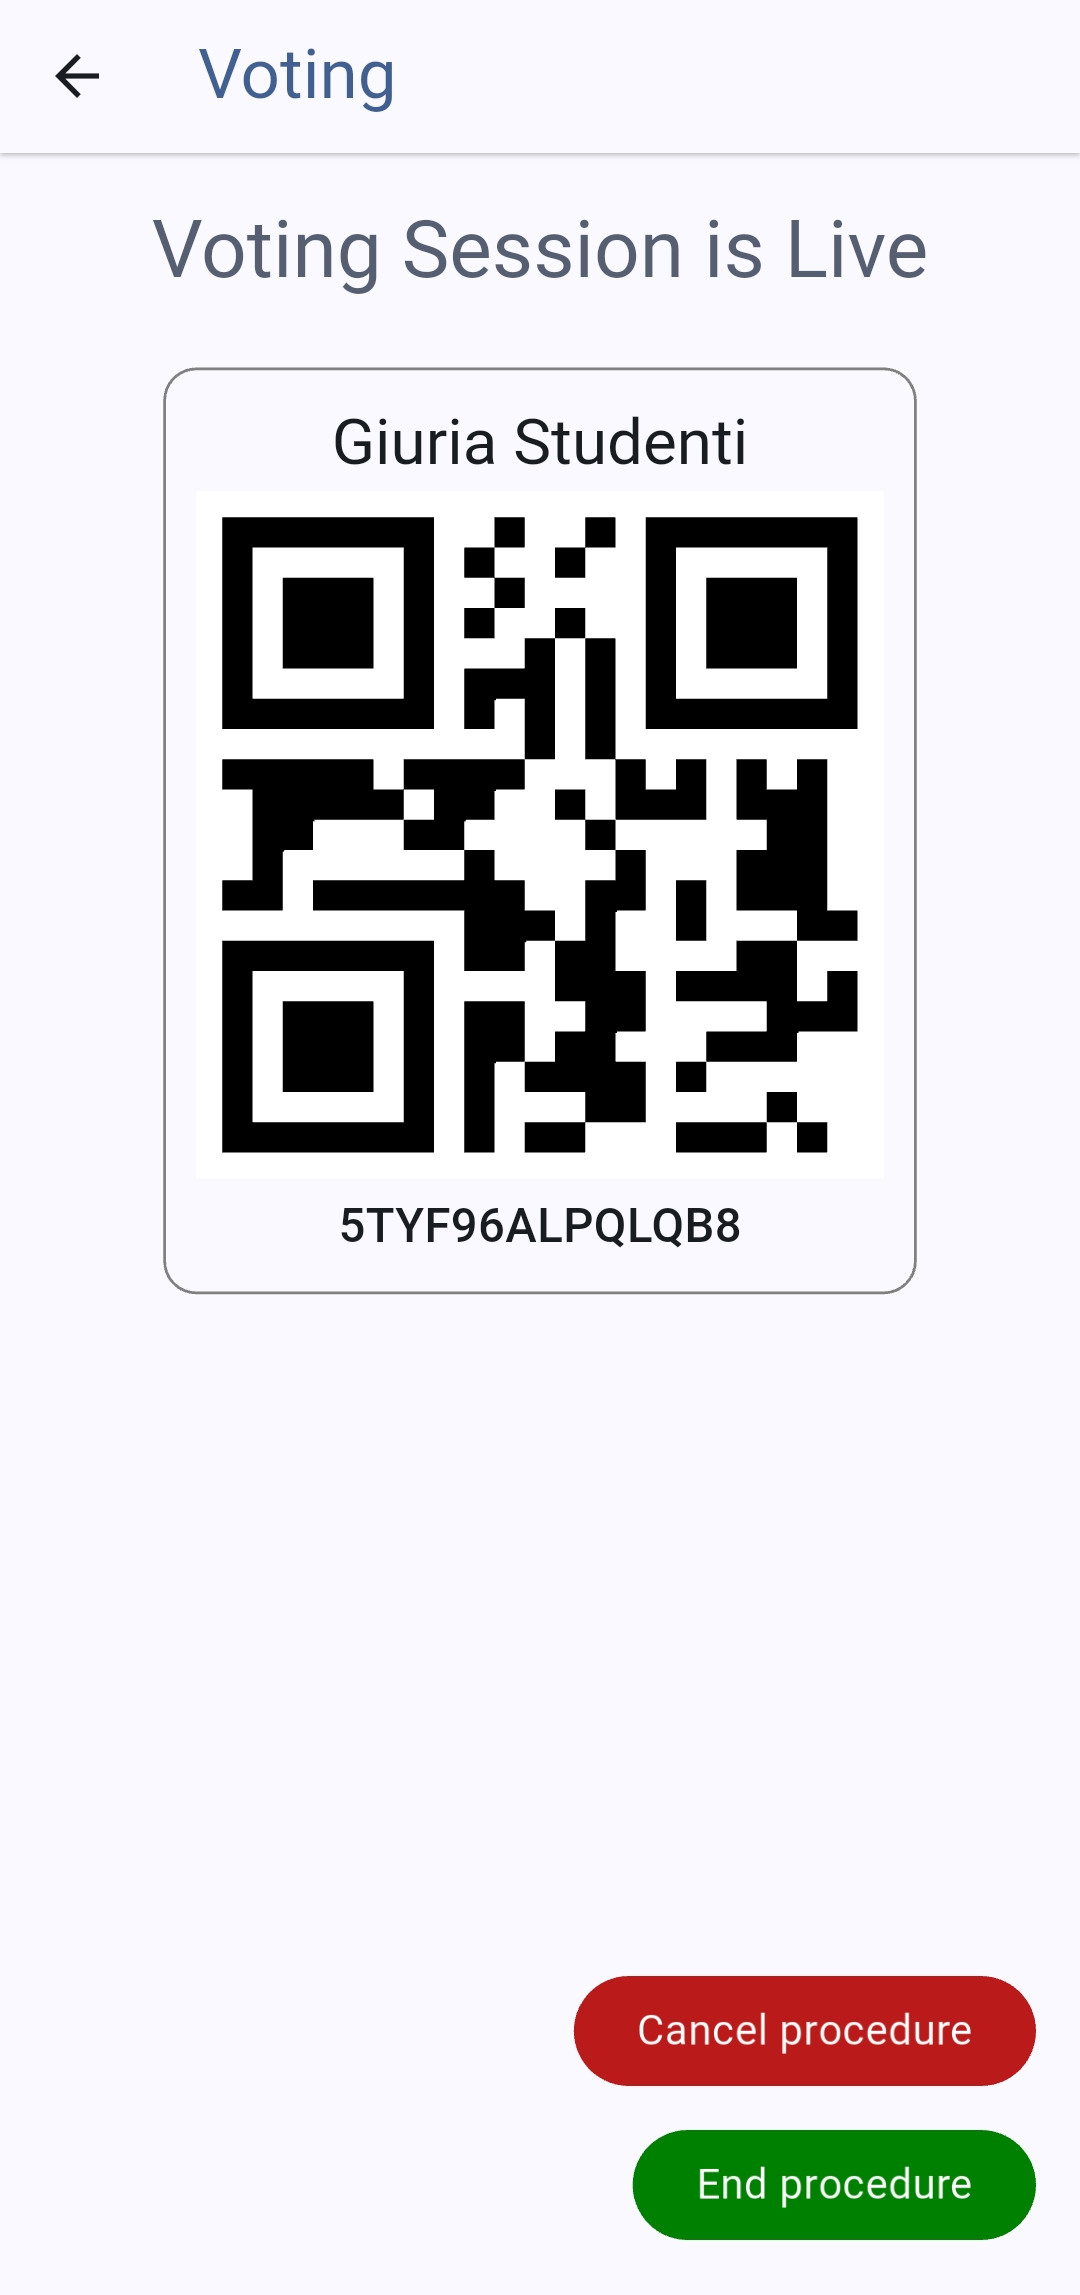
\includegraphics[width=0.4\textwidth]{figure/organizer-voting-session-live}
    \caption{La schermata di una sessione di voto attiva (\emph{Live}).}
    \label{fig:voting-session-live}
\end{figure}

\paragraph{Analisi dei Risultati e Classifiche}
Terminata la votazione, la tab \textbf{Results} permette all'organizzatore di analizzare i dati.
Può esplorare le \textbf{sottomissioni dei voti} di ciascun giurato, visualizzando le risposte fornite per ogni sezione del form (header, participant, footer).
Successivamente può \textbf{generare una classifica} per una specifica giuria, selezionando i campi di tipo slider da includere nel calcolo.

% --- FIGURE: Risultati e Classifiche (3+1 immagini) ---
\begin{figure}[H]
    \centering
    \begin{minipage}[t]{0.30\textwidth}
        \centering
        
\includegraphics[width=\linewidth]{figure/organizer-voting-results-header}
        \subcaption{Voti Header}
        \label{fig:results_header}
    \end{minipage}\hfill
    \begin{minipage}[t]{0.30\textwidth}
        \centering
        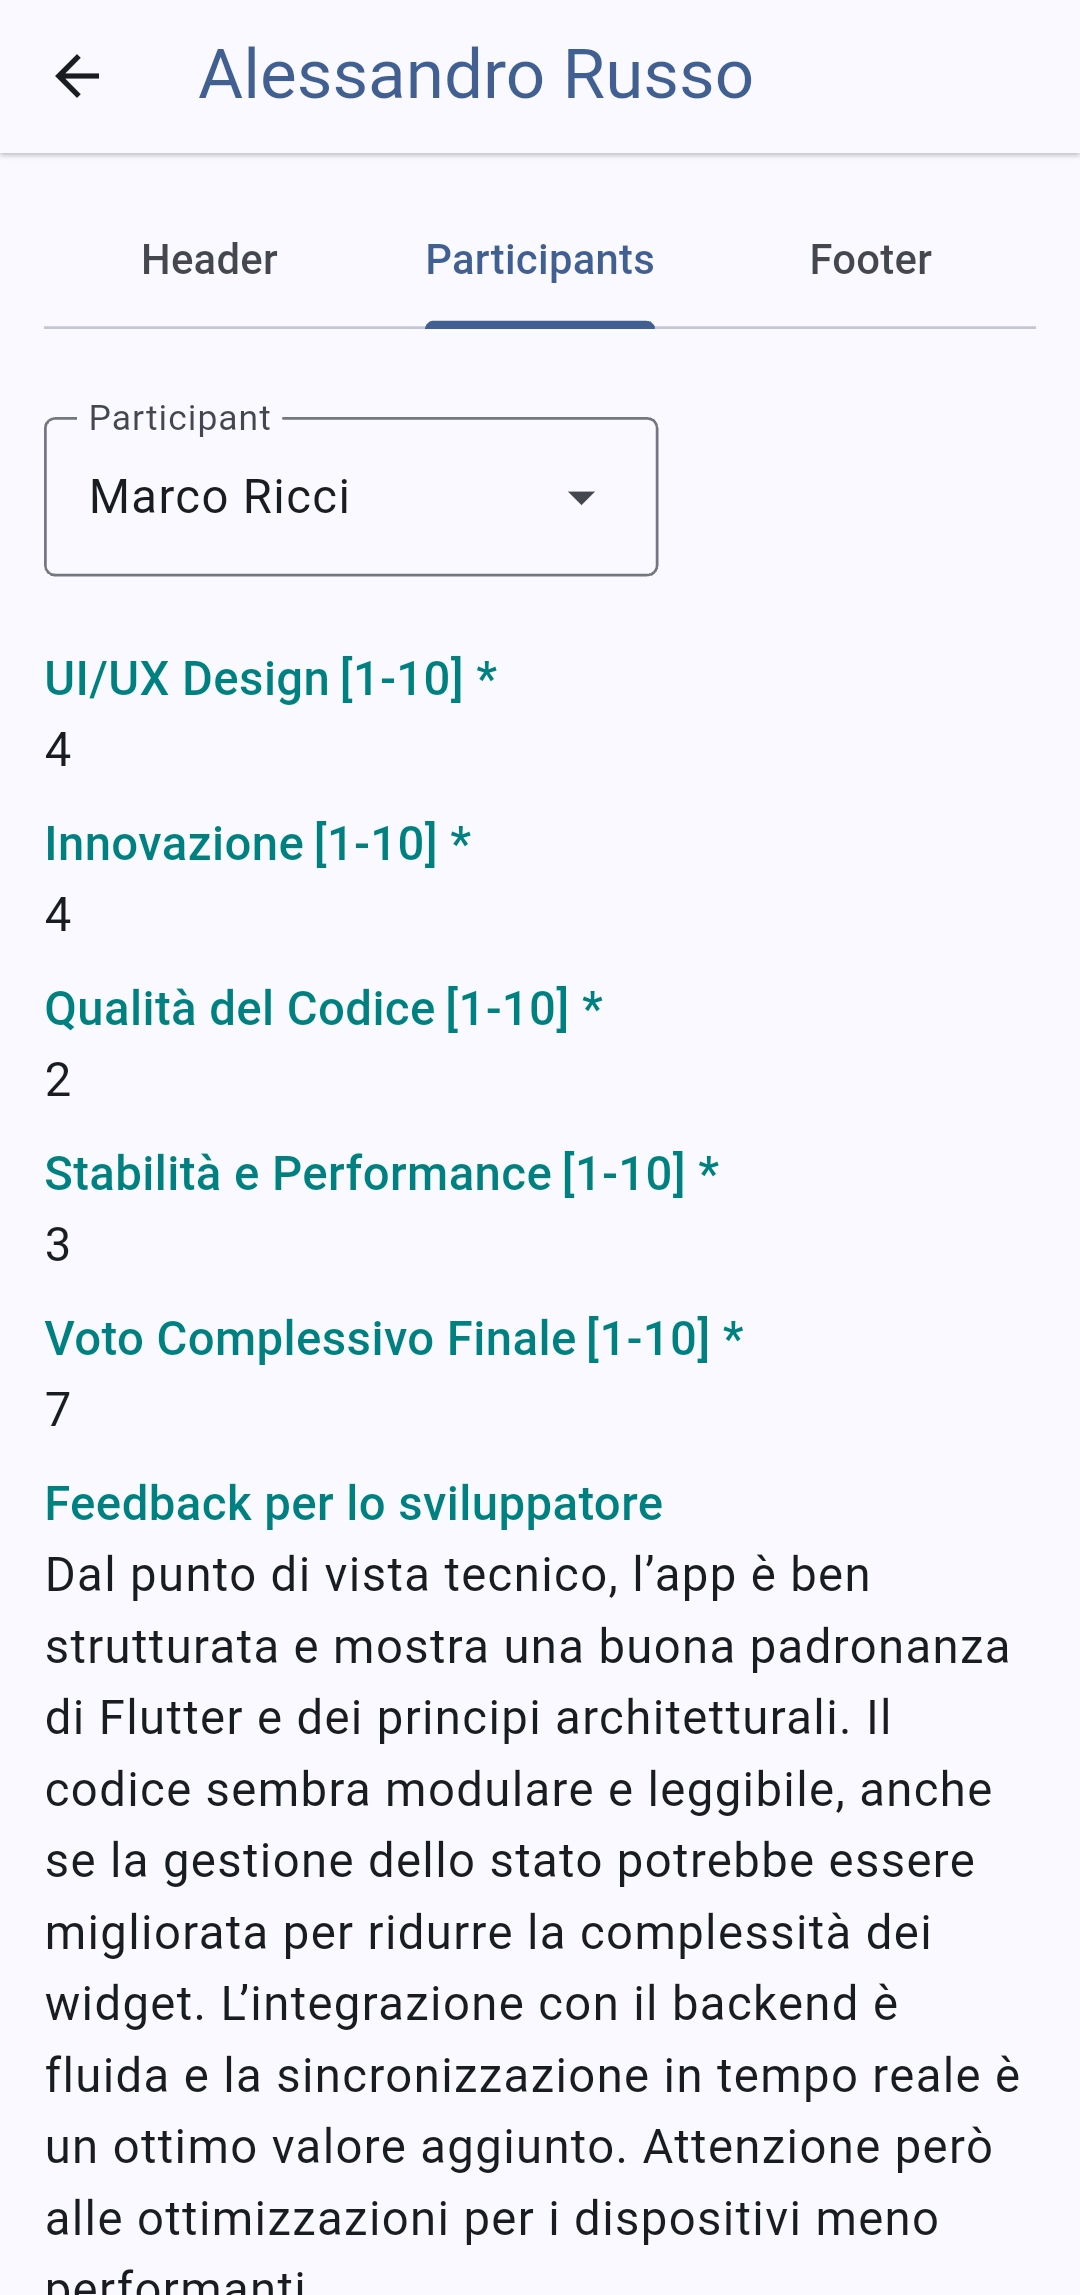
\includegraphics[width=\linewidth]{figure/organizer-voting-results-participant}
        \subcaption{Voti Participant}
        \label{fig:results_participant}
    \end{minipage}\hfill
    \begin{minipage}[t]{0.30\textwidth}
        \centering
        
\includegraphics[width=\linewidth]{figure/organizer-voting-results-footer}
        \subcaption{Voti Footer}
        \label{fig:results_footer}
    \end{minipage}
    \caption{Visualizzazione dei voti inviati da un giurato, suddivisi per scope.}
    \label{fig:results-submission-view}
\end{figure}

\begin{figure}[H]
    \centering
    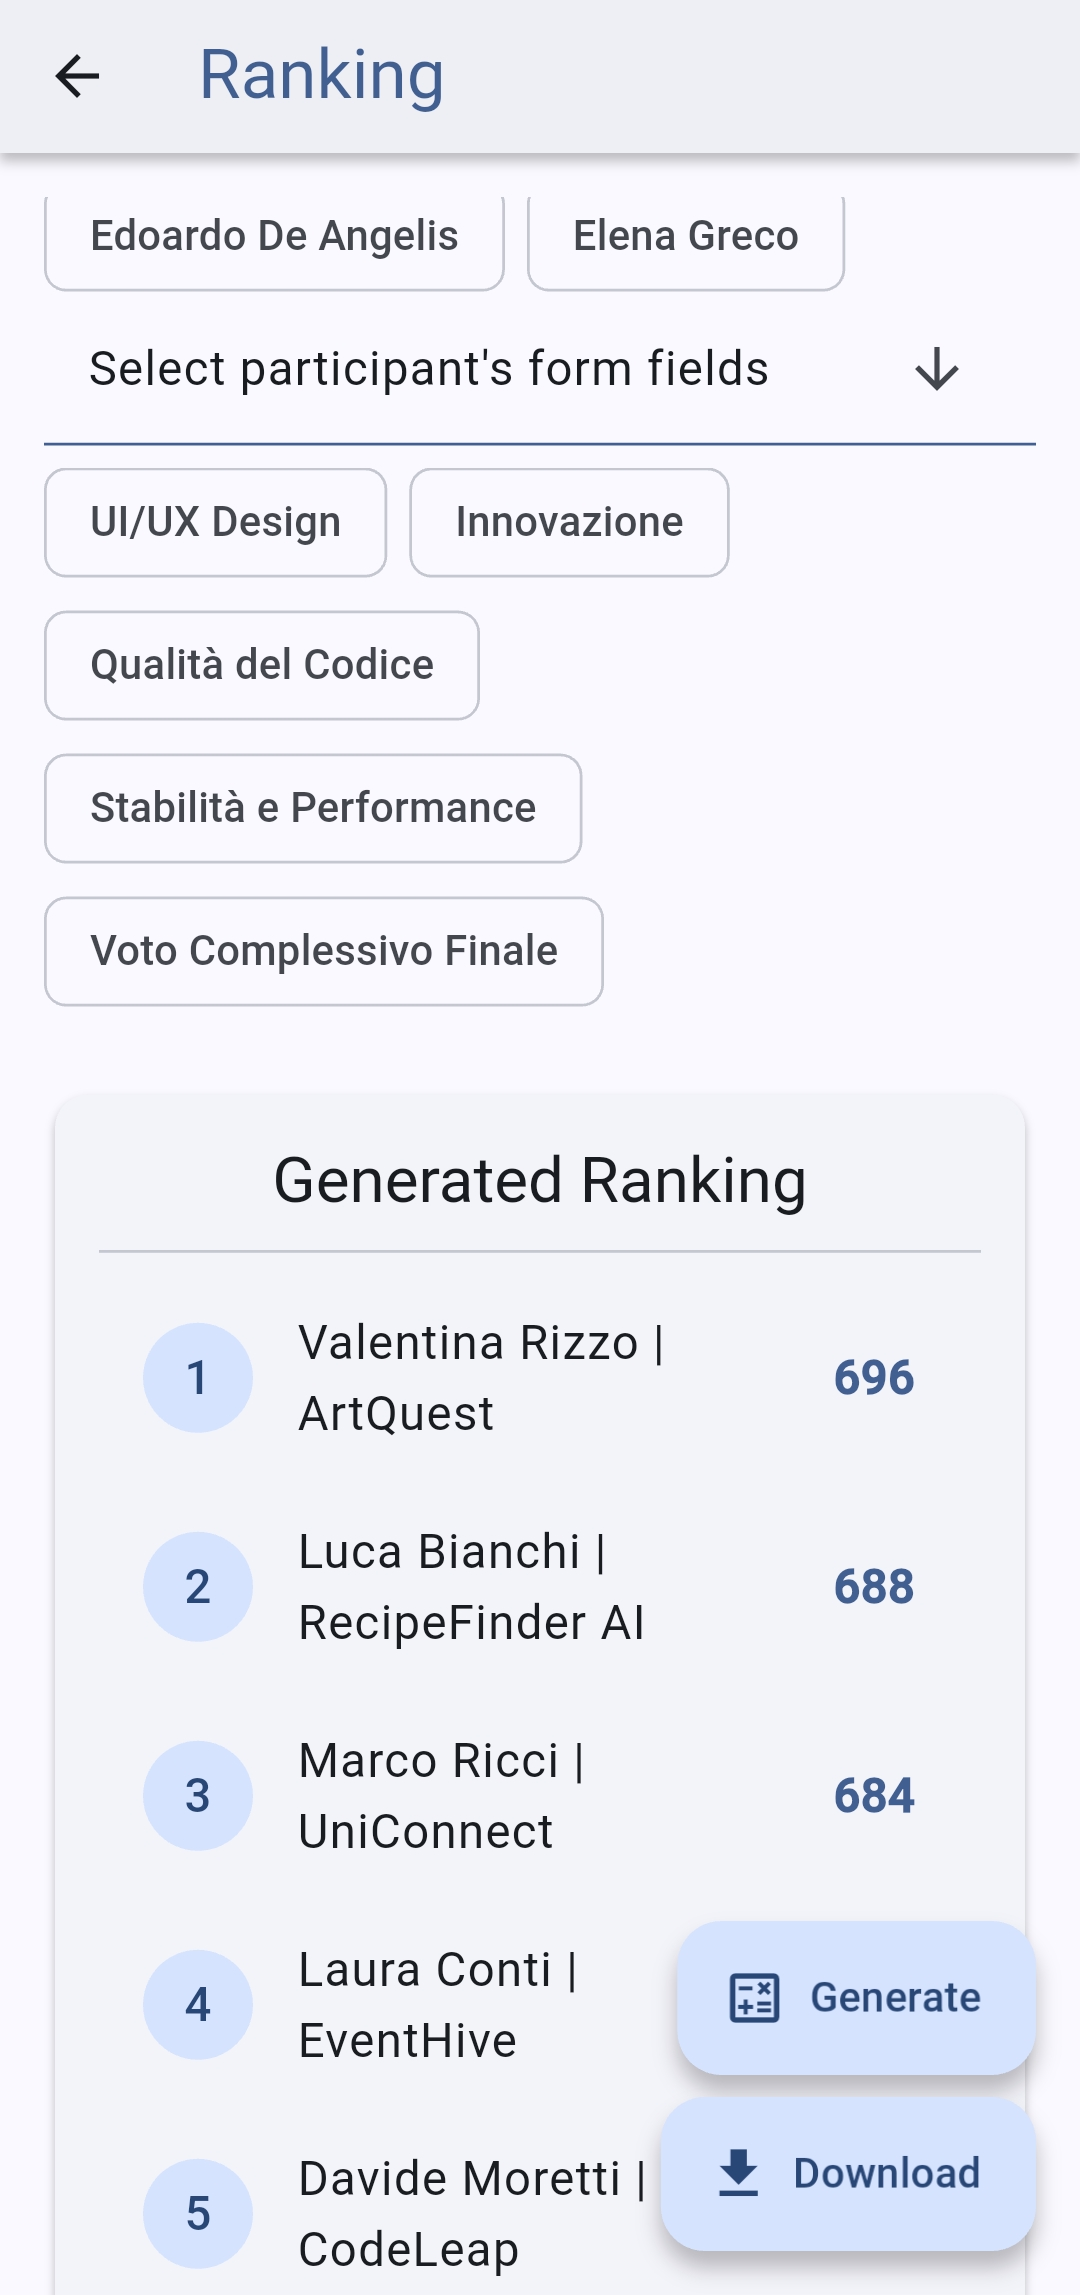
\includegraphics[width=0.4\textwidth]{figure/organizer-ranking-generation}
    \caption{La pagina per la generazione della classifica di una giuria.}
    \label{fig:ranking-generation}
\end{figure}

\subsection{Flusso del Partecipante}\label{subsec:flusso-del-partecipante}
Il partecipante, una volta accettato l'invito a un concorso, ha un percorso chiaro e focalizzato.
La sua azione principale è la \textbf{sottomissione del proprio \emph{Work}} prima della scadenza.

Un form guidato lo accompagna nel processo di caricamento, suddiviso in tre passaggi:
\begin{enumerate}
    \item Inserimento dei dati principali: \textbf{nome} e \textbf{descrizione} dell'opera.
    \item Caricamento delle \textbf{immagini di anteprima}, che verranno mostrate ai giurati durante la votazione.
    \item Caricamento del \textbf{file \texttt{.zip}} contenente il materiale completo del lavoro.
\end{enumerate}

% --- FIGURE: Sottomissione del Work (3 immagini affiancate) ---
\begin{figure}[H]
    \centering
    \begin{minipage}[t]{0.30\textwidth}
        \centering
        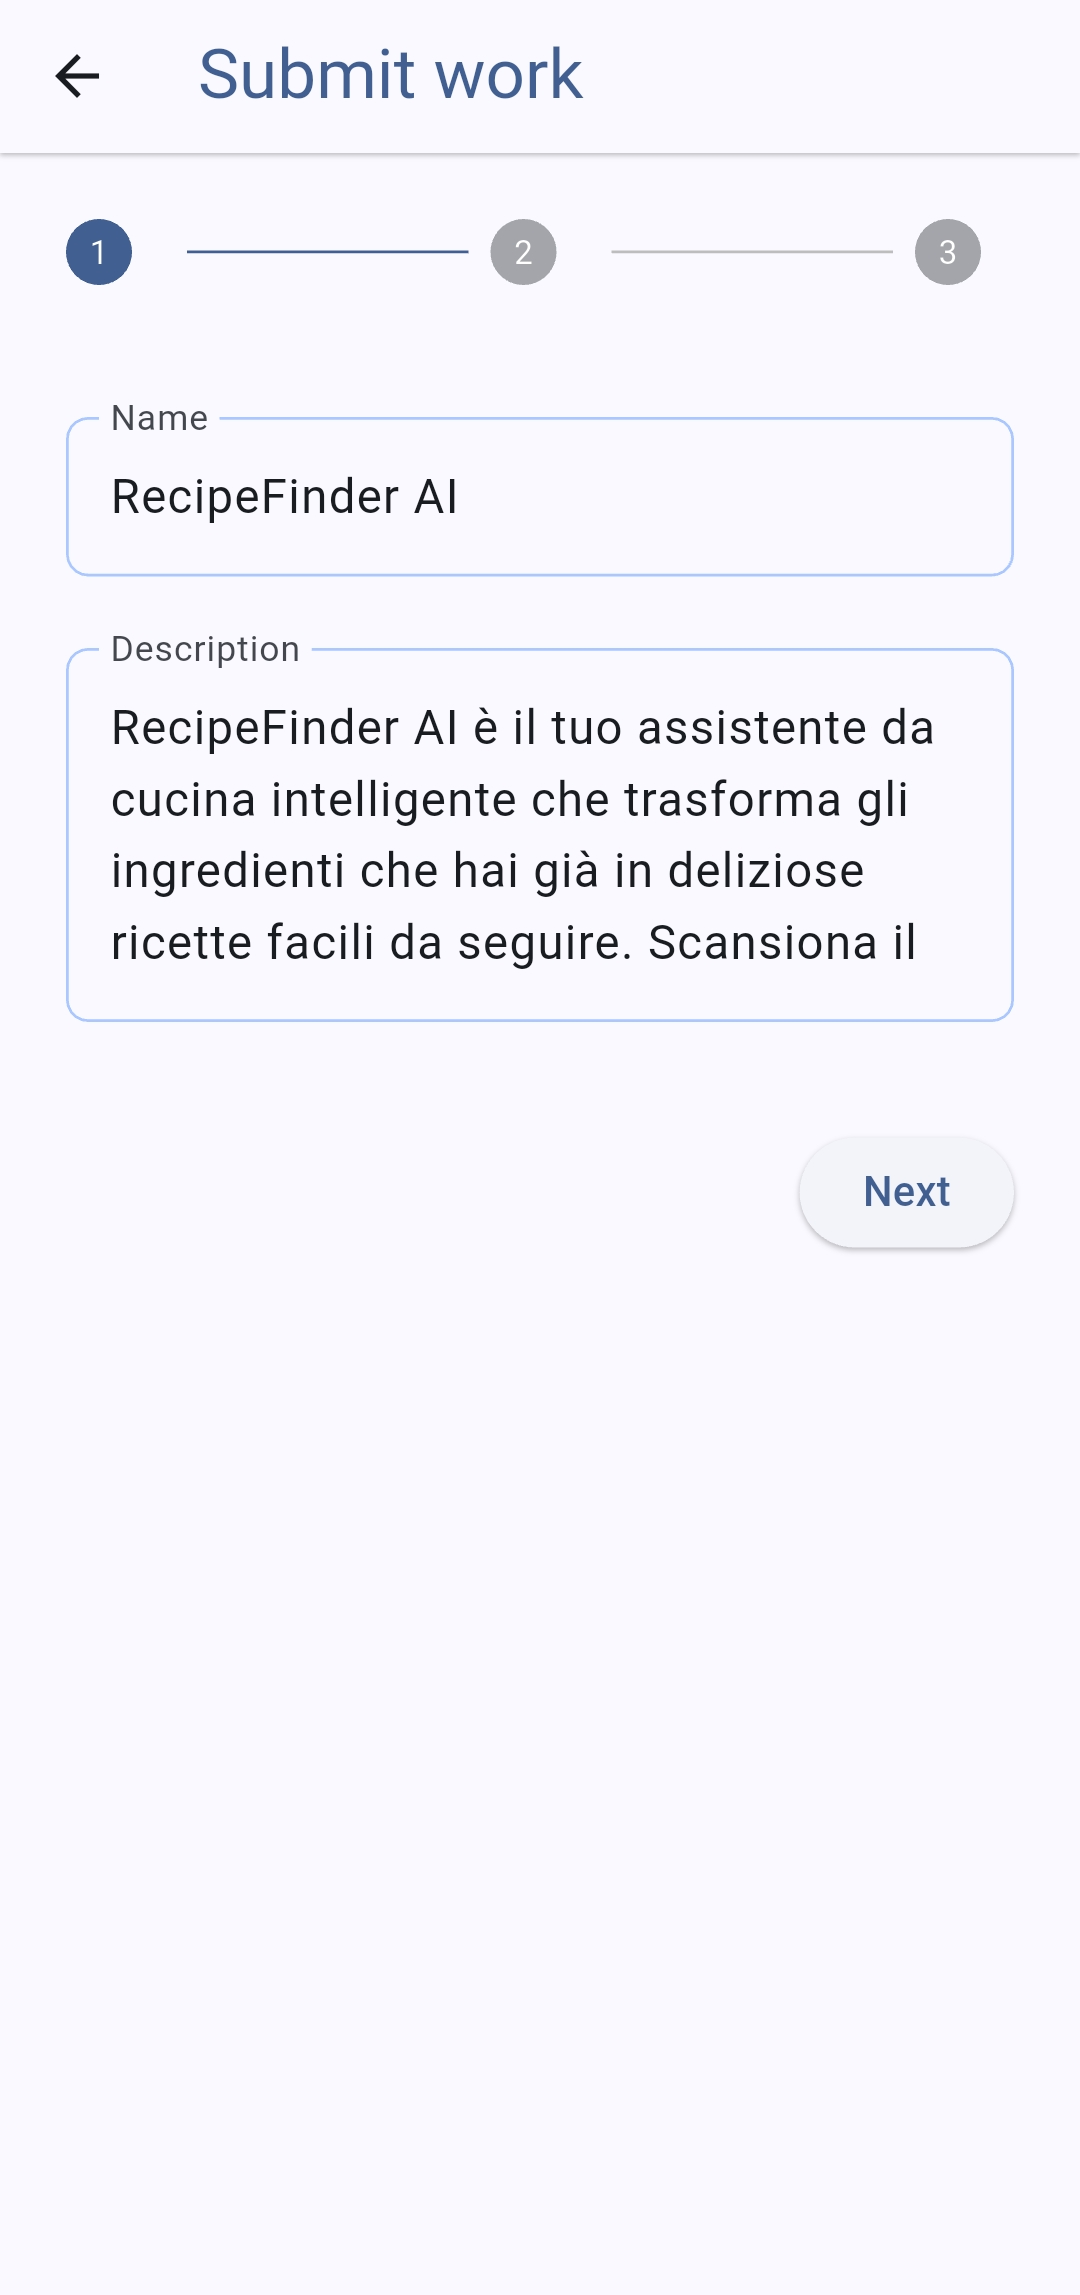
\includegraphics[width=\linewidth]{figure/participant-submit-work-step1}
        \subcaption{Passo 1: Dati}
        \label{fig:submit_work_1}
    \end{minipage}\hfill
    \begin{minipage}[t]{0.30\textwidth}
        \centering
        
\includegraphics[width=\linewidth]{figure/participant-submit-work-step2}
        \subcaption{Passo 2: Immagini}
        \label{fig:submit_work_2}
    \end{minipage}\hfill
    \begin{minipage}[t]{0.30\textwidth}
        \centering
        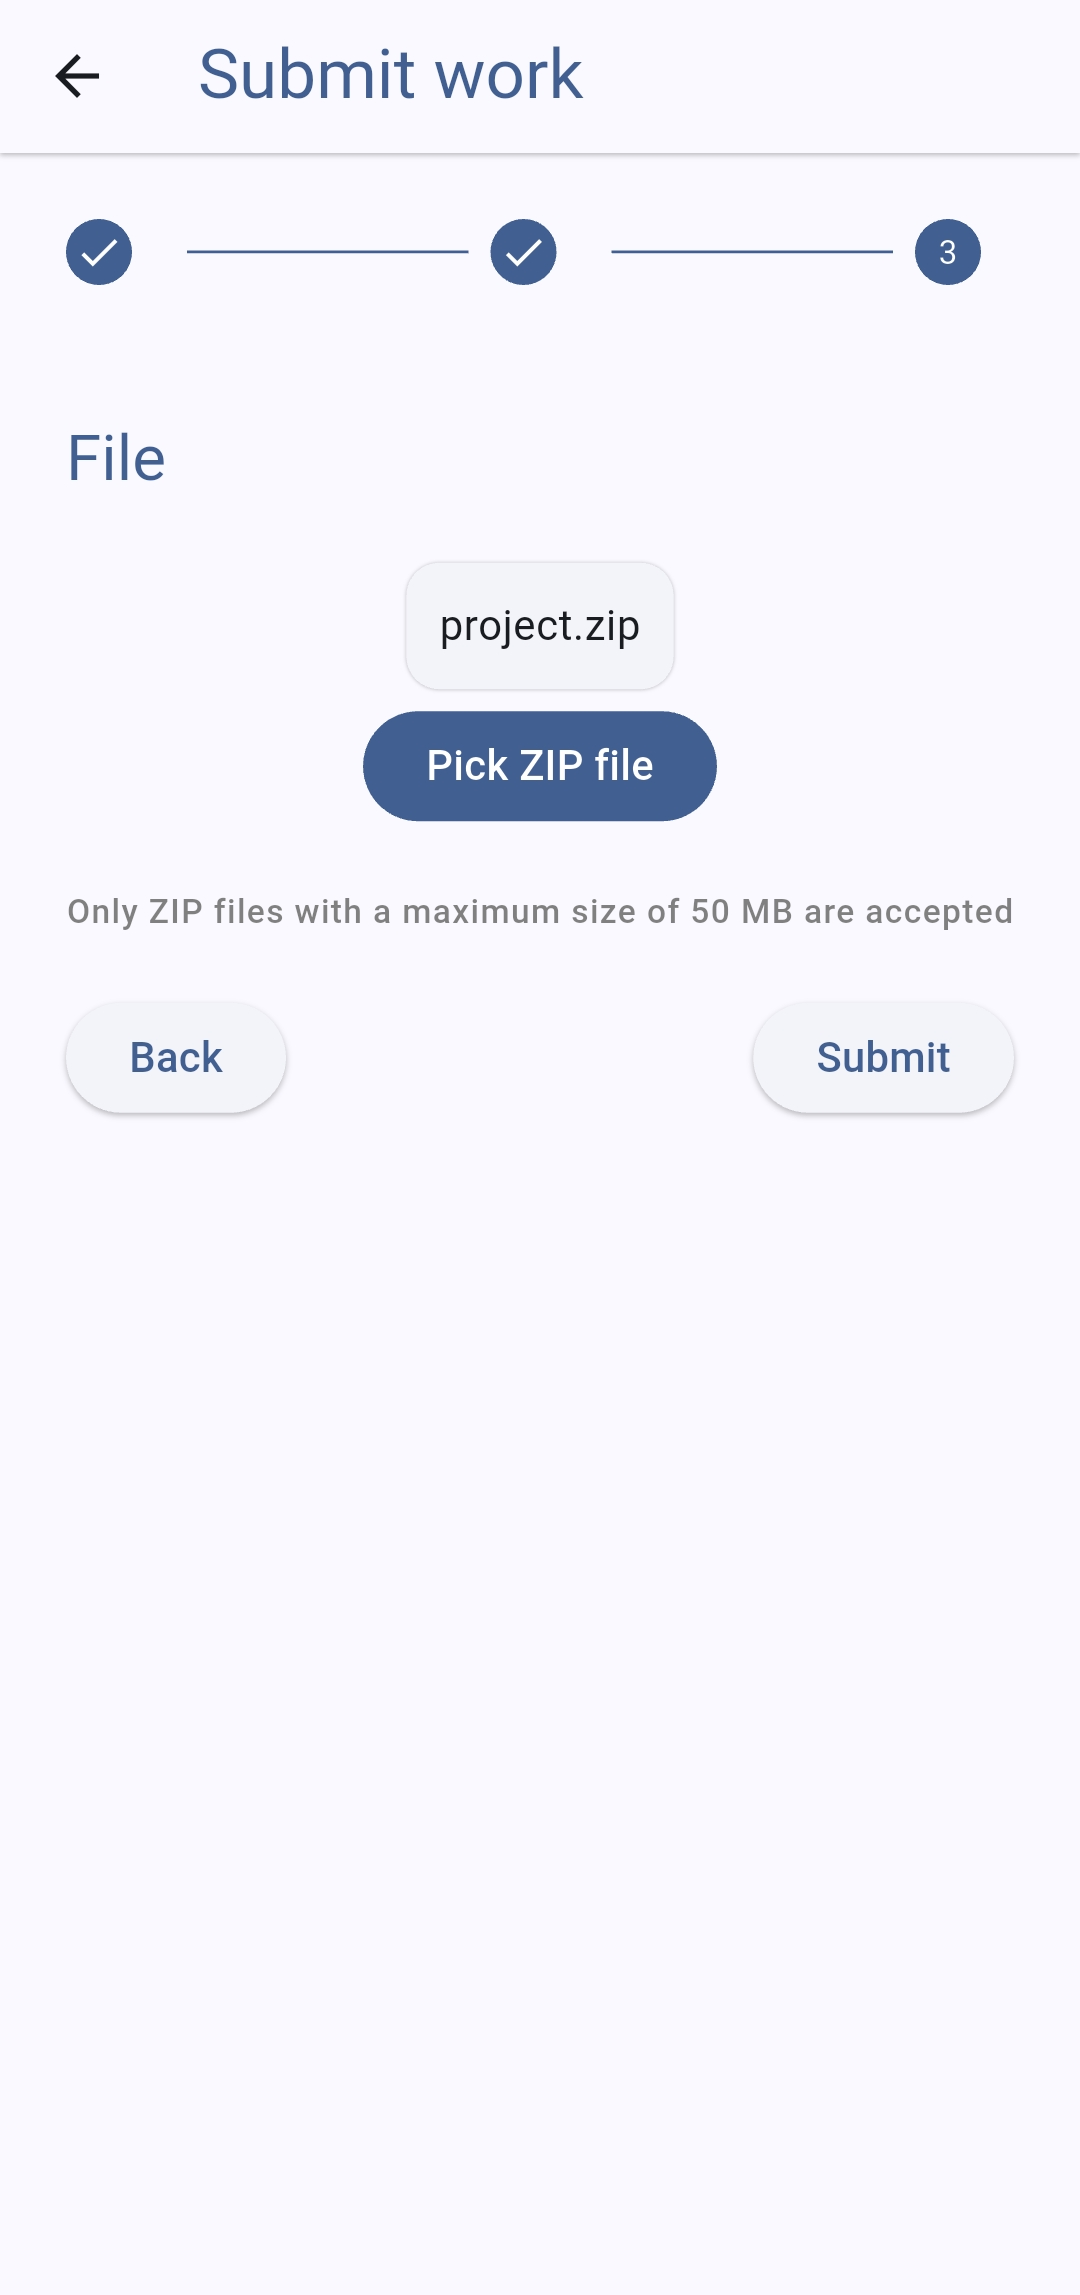
\includegraphics[width=\linewidth]{figure/participant-submit-work-step3}
        \subcaption{Passo 3: File}
        \label{fig:submit_work_3}
    \end{minipage}
    \caption{Le tre schermate del form guidato per la sottomissione di un \emph{Work}.}
    \label{fig:submit_work_flow}
\end{figure}

Una volta completata la sottomissione, accedendo alla pagina di dettaglio del contest, il partecipante può visualizzare un riepilogo del lavoro caricato all'interno della tab \textbf{Work}.

% --- FIGURA: Tab Work con lavoro sottomesso ---
\begin{figure}[H]
    \centering
    
\includegraphics[width=0.4\textwidth]{figure/participant-submitted-work}
    \caption{La tab ``Work'' del partecipante dopo aver sottomesso la propria opera.}
    \label{fig:participant_work_submitted}
\end{figure}

\subsection{Flusso del Giurato}\label{subsec:flusso-del-giurato}
Il flusso del giurato è progettato per essere semplice e focalizzato sull'unica azione richiesta: la votazione.
Il sistema supporta sia i giurati nominati (\emph{appointed}) che quelli semplici (\emph{simple}).

Un \textbf{giurato}, dopo l'autenticazione, accede alla sua \textbf{Home Page}, dove visualizza l'elenco dei contest di cui fa parte, cioè di cui è un giurato nominato.

% --- FIGURA: Home Page Giurato ---
\begin{figure}[H]
    \centering
    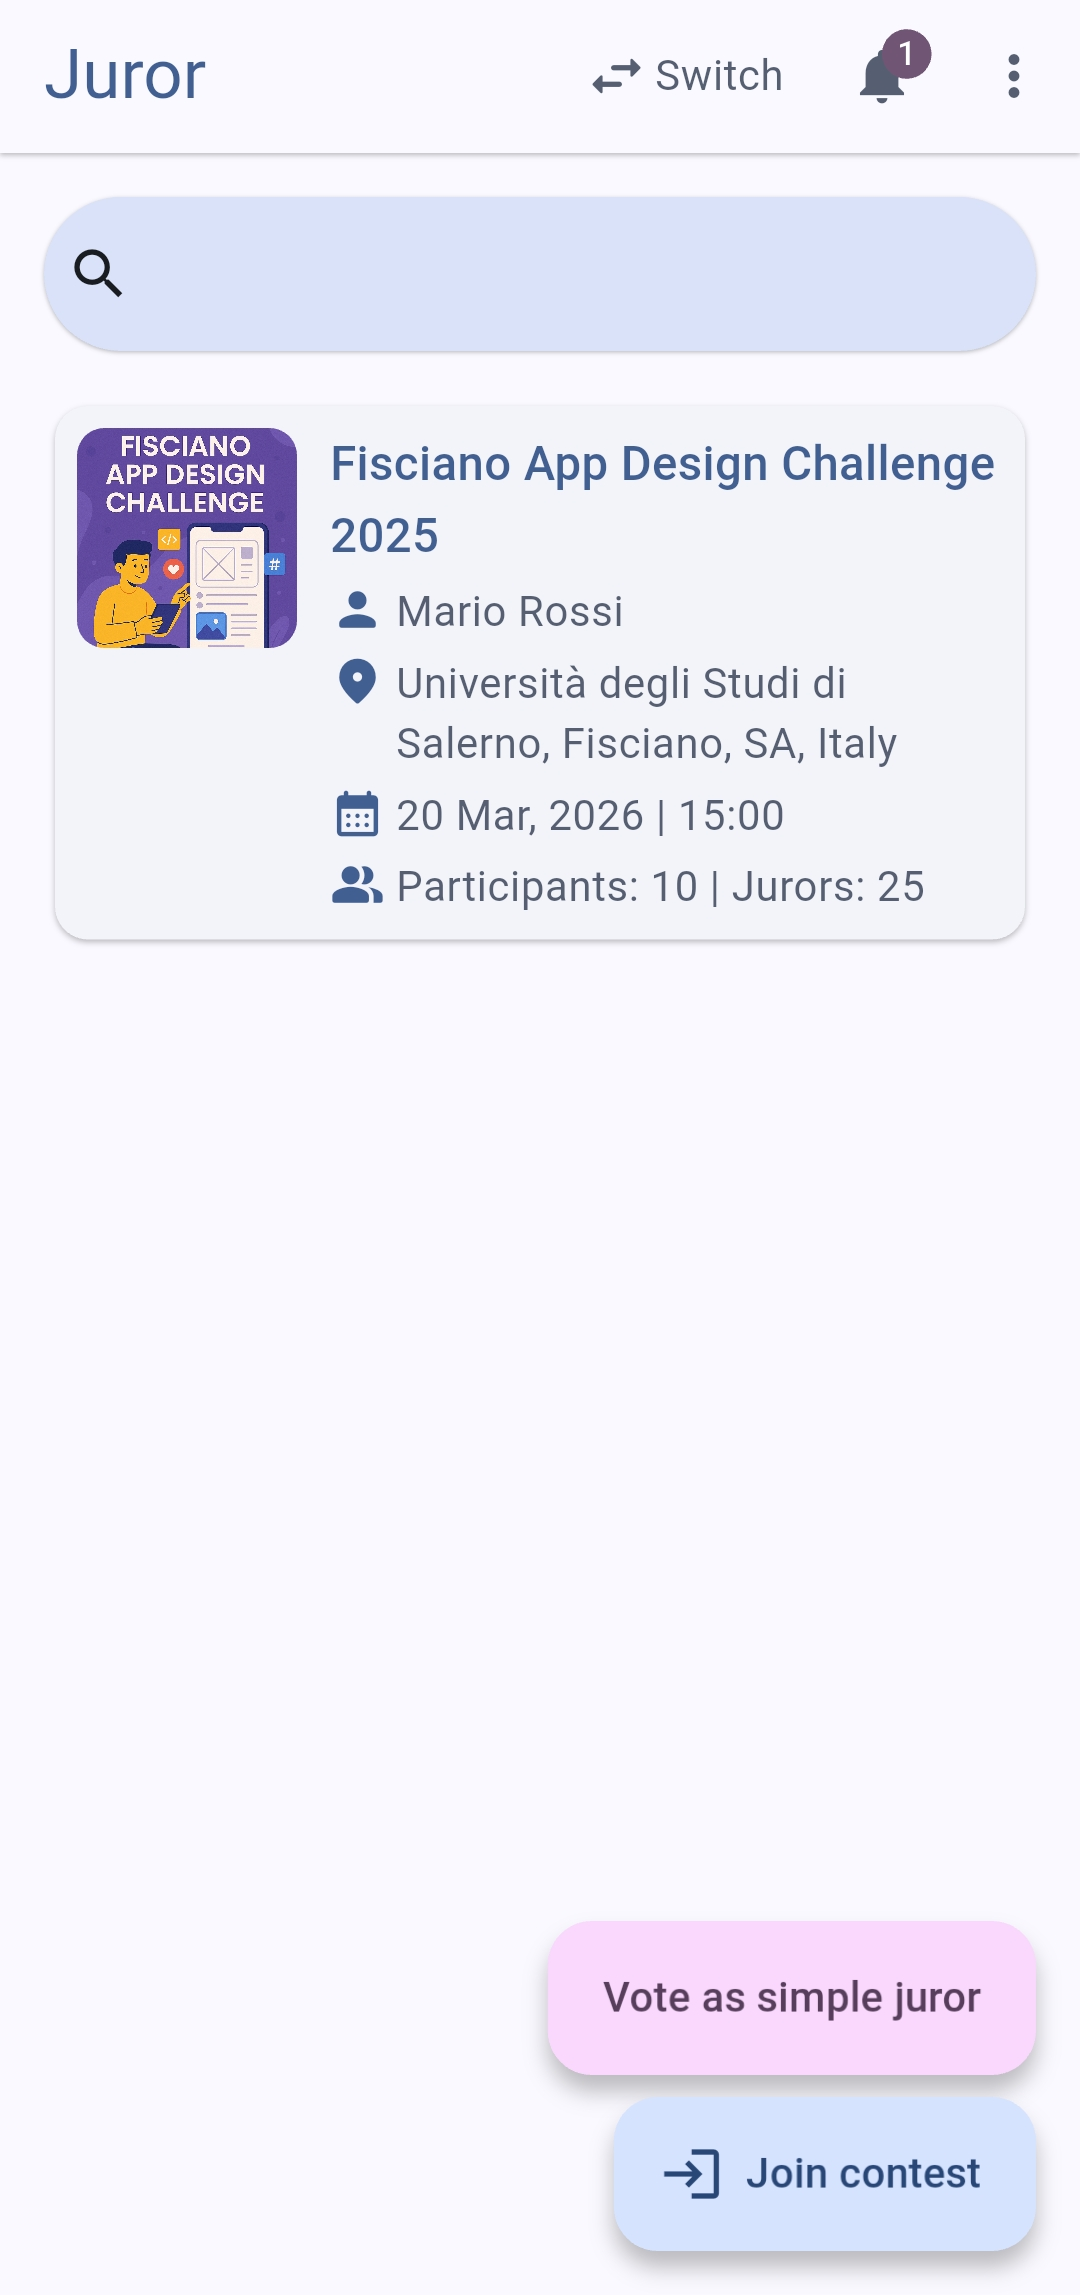
\includegraphics[width=0.4\textwidth]{figure/juror-home}
    \caption{La Home Page del Giurato, con la possibilità di votare come giurato semplice.}
    \label{fig:juror_home}
\end{figure}

Quando un organizzatore avvia una sessione di voto, il giurato riceve una notifica in tempo reale nella sua \textbf{Inbox}.

% --- FIGURA: Notifica Inbox ---
\begin{figure}[H]
    \centering
    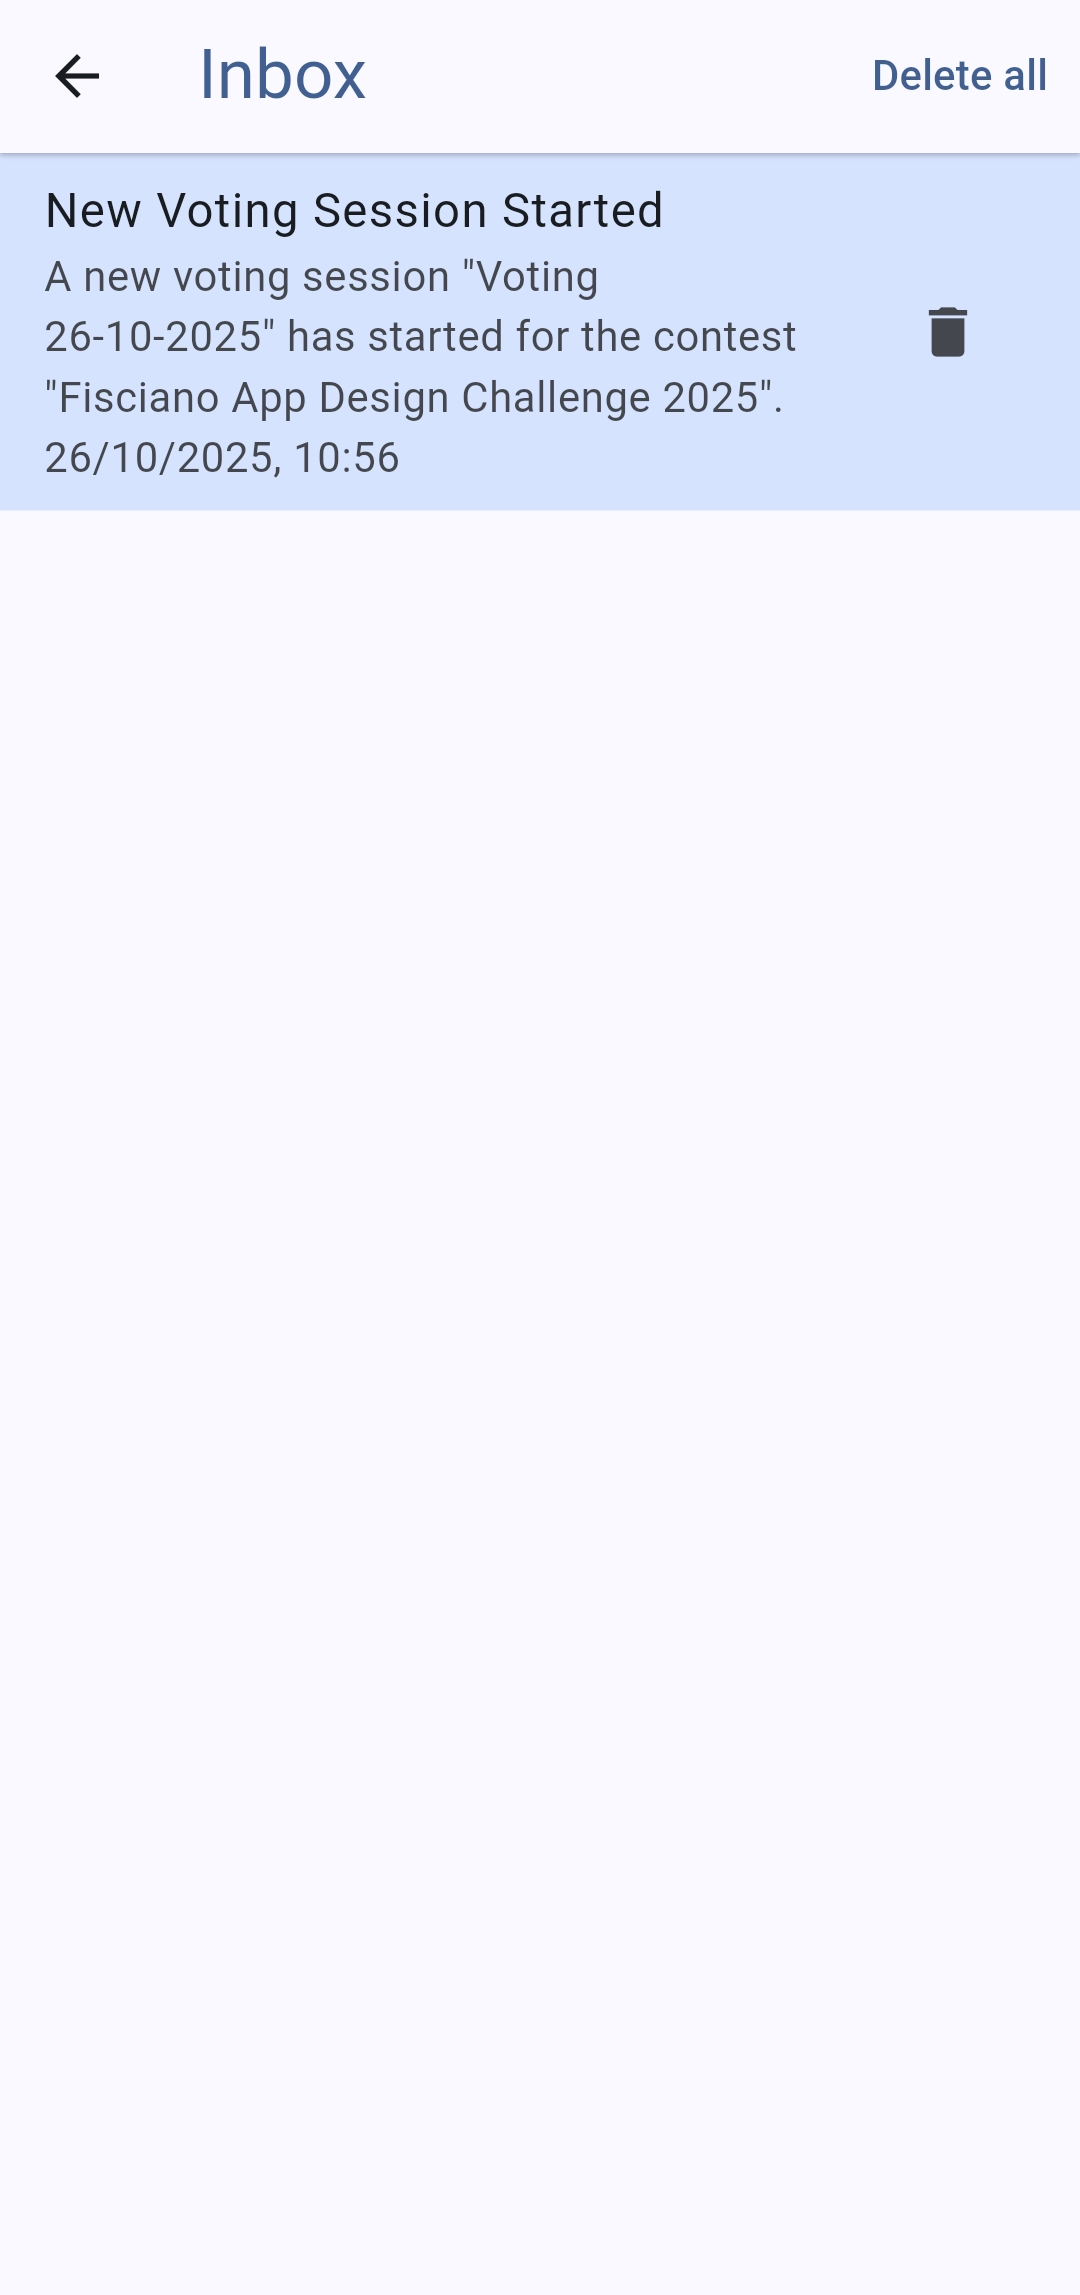
\includegraphics[width=0.4\textwidth]{figure/juror-inbox-notification}
    \caption{La pagina Inbox che mostra la notifica di avvio di una sessione di voto.}
    \label{fig:juror_inbox}
\end{figure}

Nella pagina dei dettagli del contest, se una sessione di voto è attiva (\emph{live}), il giurato può accedere alla votazione attraverso un apposito tasto.

% --- FIGURA: Dettagli Contest con Tasto "Vote" ---
\begin{figure}[H]
    \centering
    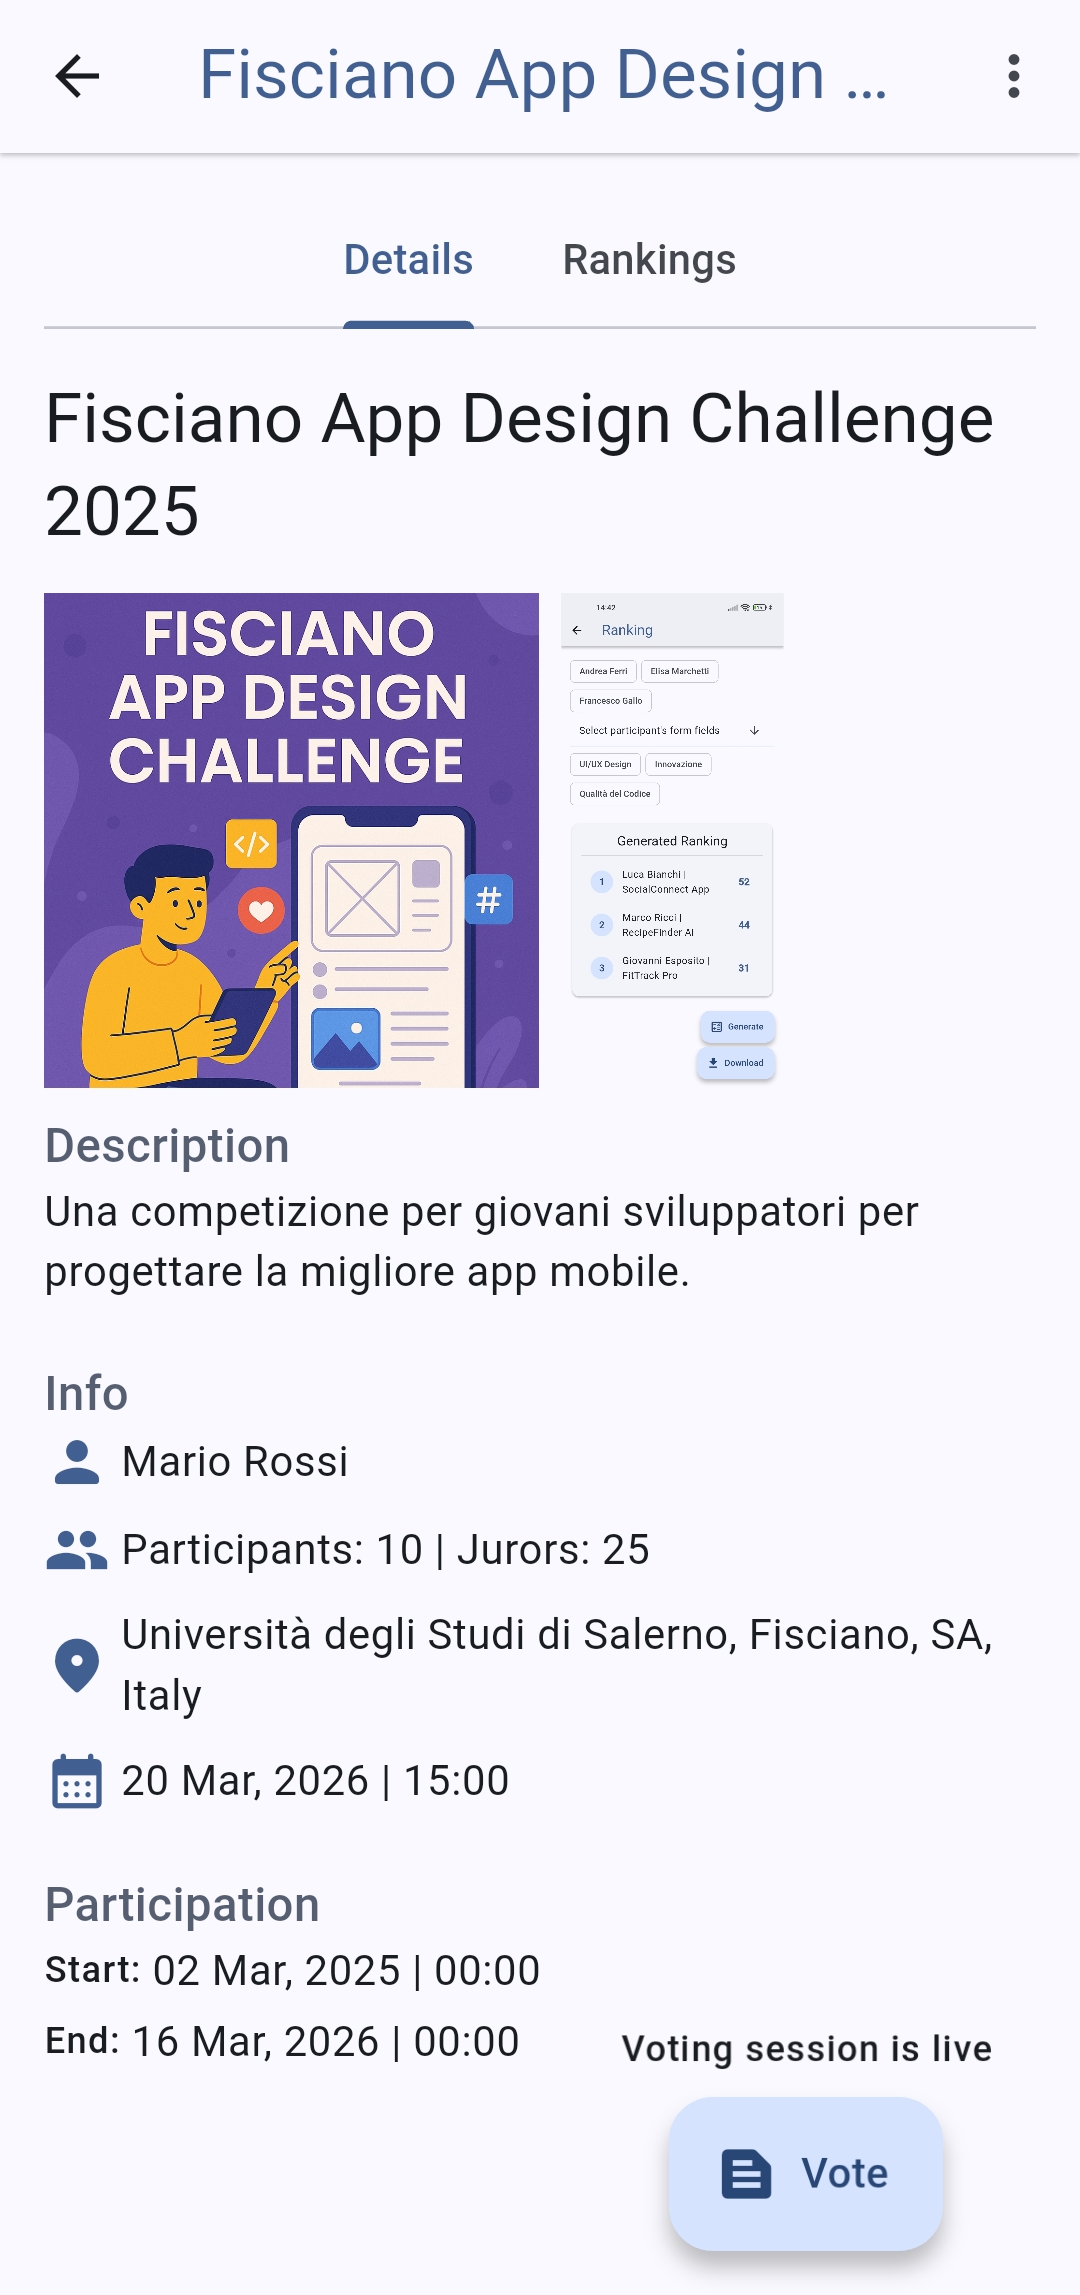
\includegraphics[width=0.4\textwidth]{figure/juror-contest-details}
    \caption{La pagina di dettaglio del contest per un giurato, con il pulsante per accedere alla votazione live.}
    \label{fig:juror_contest_details_vote}
\end{figure}

\paragraph{Procedura di Votazione}
La procedura di votazione guida il giurato attraverso una serie di schermate strutturate, basate sulla configurazione del \emph{VotingForm}:
\begin{enumerate}
    \item Una \textbf{schermata introduttiva} presenta il nome e la descrizione del form di voto.
    \item Seguono i campi con scope \textbf{Header}, da compilare una sola volta.
    \item Il sistema itera poi su tutti i partecipanti inclusi nella sessione.
    Per ciascuno, viene mostrata una schermata con i dettagli del \emph{Work} e i campi con scope \textbf{Participant} da compilare.
    \item Infine, vengono presentati i campi con scope \textbf{Footer}, da compilare una volta a conclusione del processo.
\end{enumerate}
Un \textbf{giurato semplice}, invece, accede a questa procedura direttamente tramite il token della giuria, saltando i passaggi precedenti.

% --- FIGURE: Procedura di Votazione (4 immagini, 2 per riga) ---
\begin{figure}[H]
    \centering
    \begin{minipage}[t]{0.30\textwidth}
        \centering
        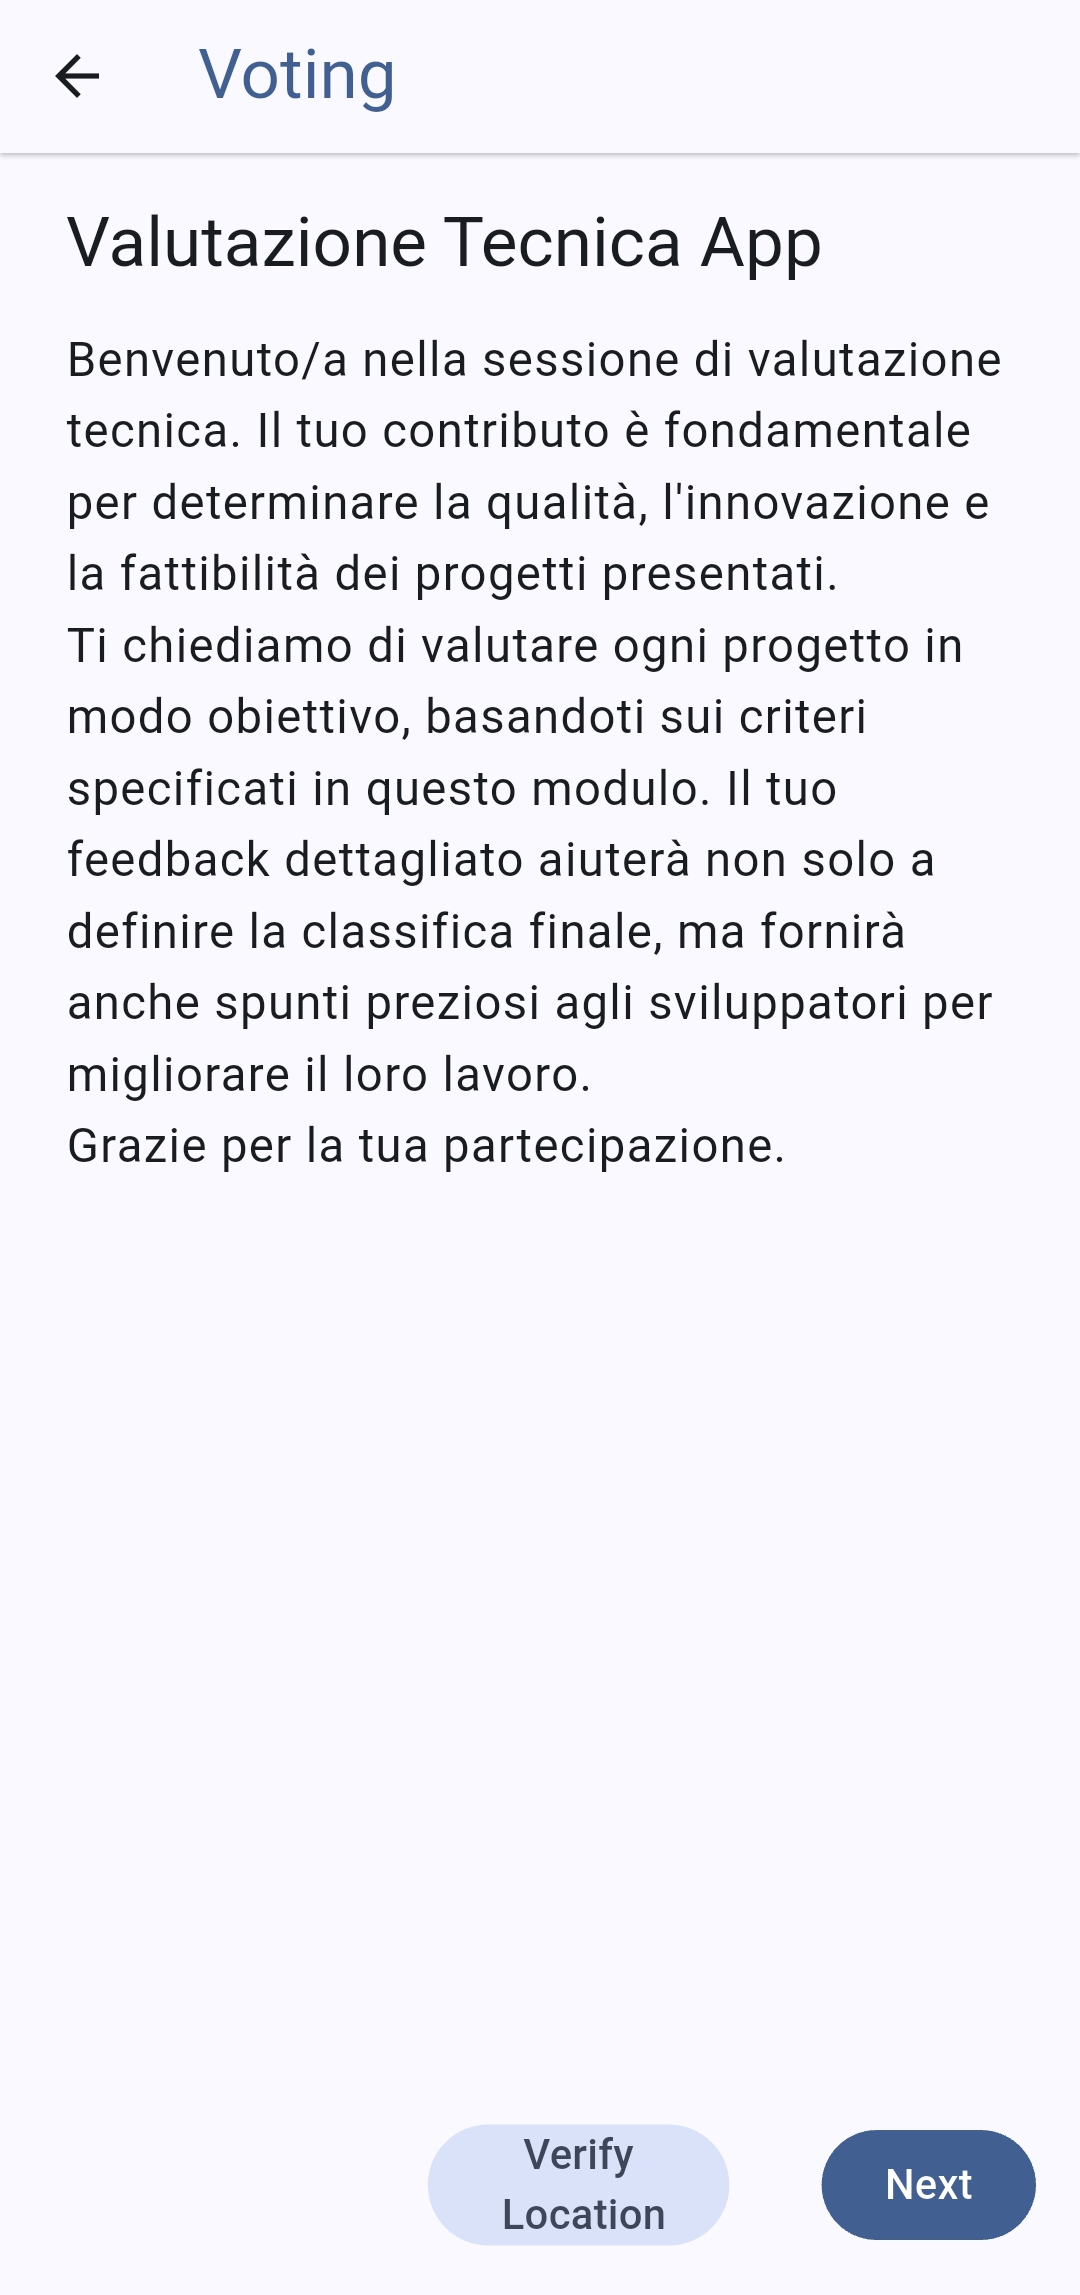
\includegraphics[width=\linewidth]{figure/juror-voting-session-intro}
        \subcaption{Schermata Introduttiva}
        \label{fig:voting_intro}
    \end{minipage}
    \quad
    \begin{minipage}[t]{0.30\textwidth}
        \centering
        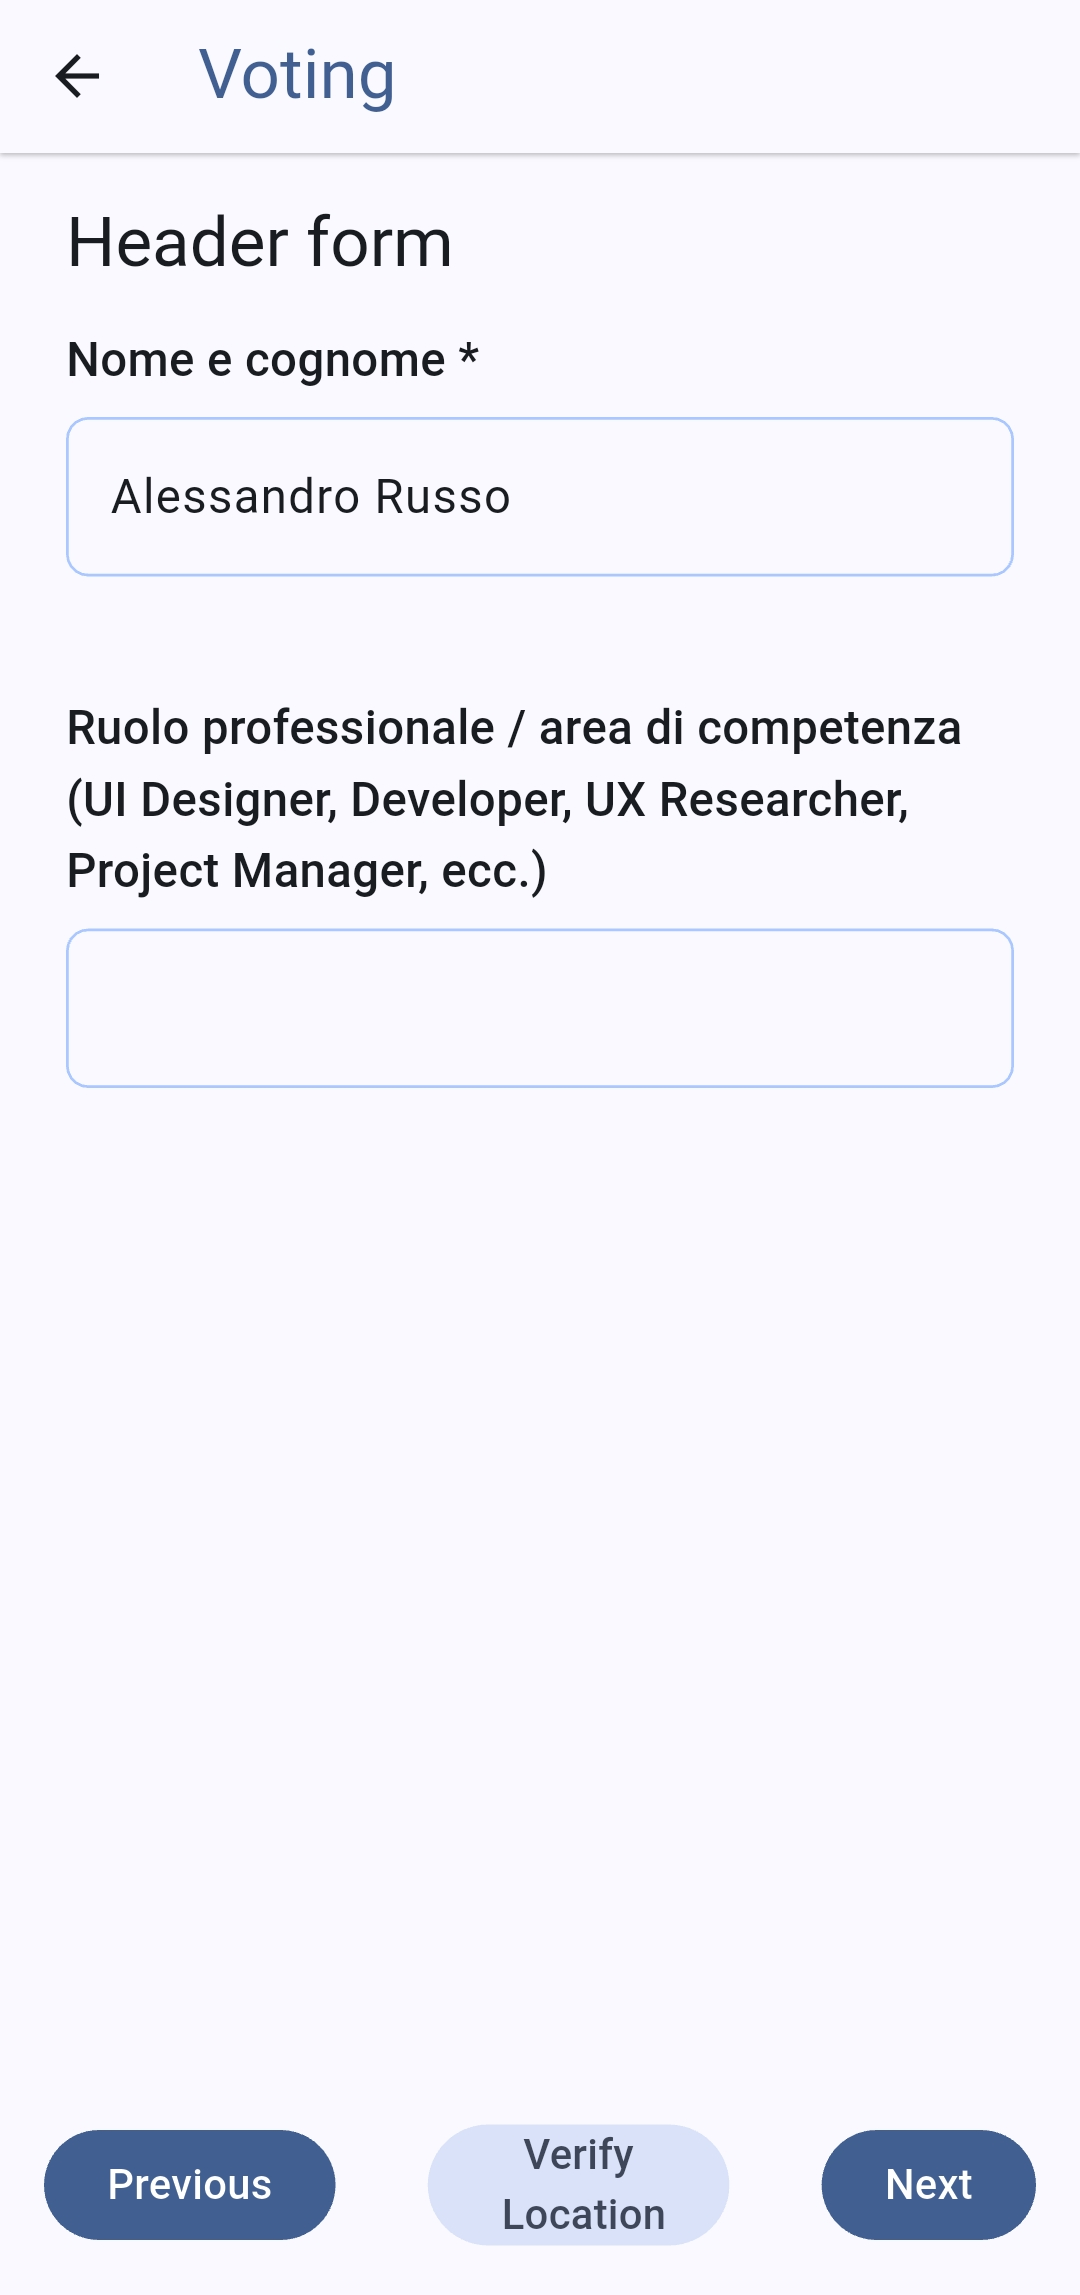
\includegraphics[width=\linewidth]{figure/juror-voting-session-header}
        \subcaption{Votazione Campi Header}
        \label{fig:voting_header}
    \end{minipage}

    \vspace{1em} % Spazio tra le righe di immagini

    \begin{minipage}[t]{0.30\textwidth}
        \centering
        
\includegraphics[width=\linewidth]{figure/juror-voting-session-participant}
        \subcaption{Votazione Campi Participant}
        \label{fig:voting_participant}
    \end{minipage}
    \quad
    \begin{minipage}[t]{0.30\textwidth}
        \centering
        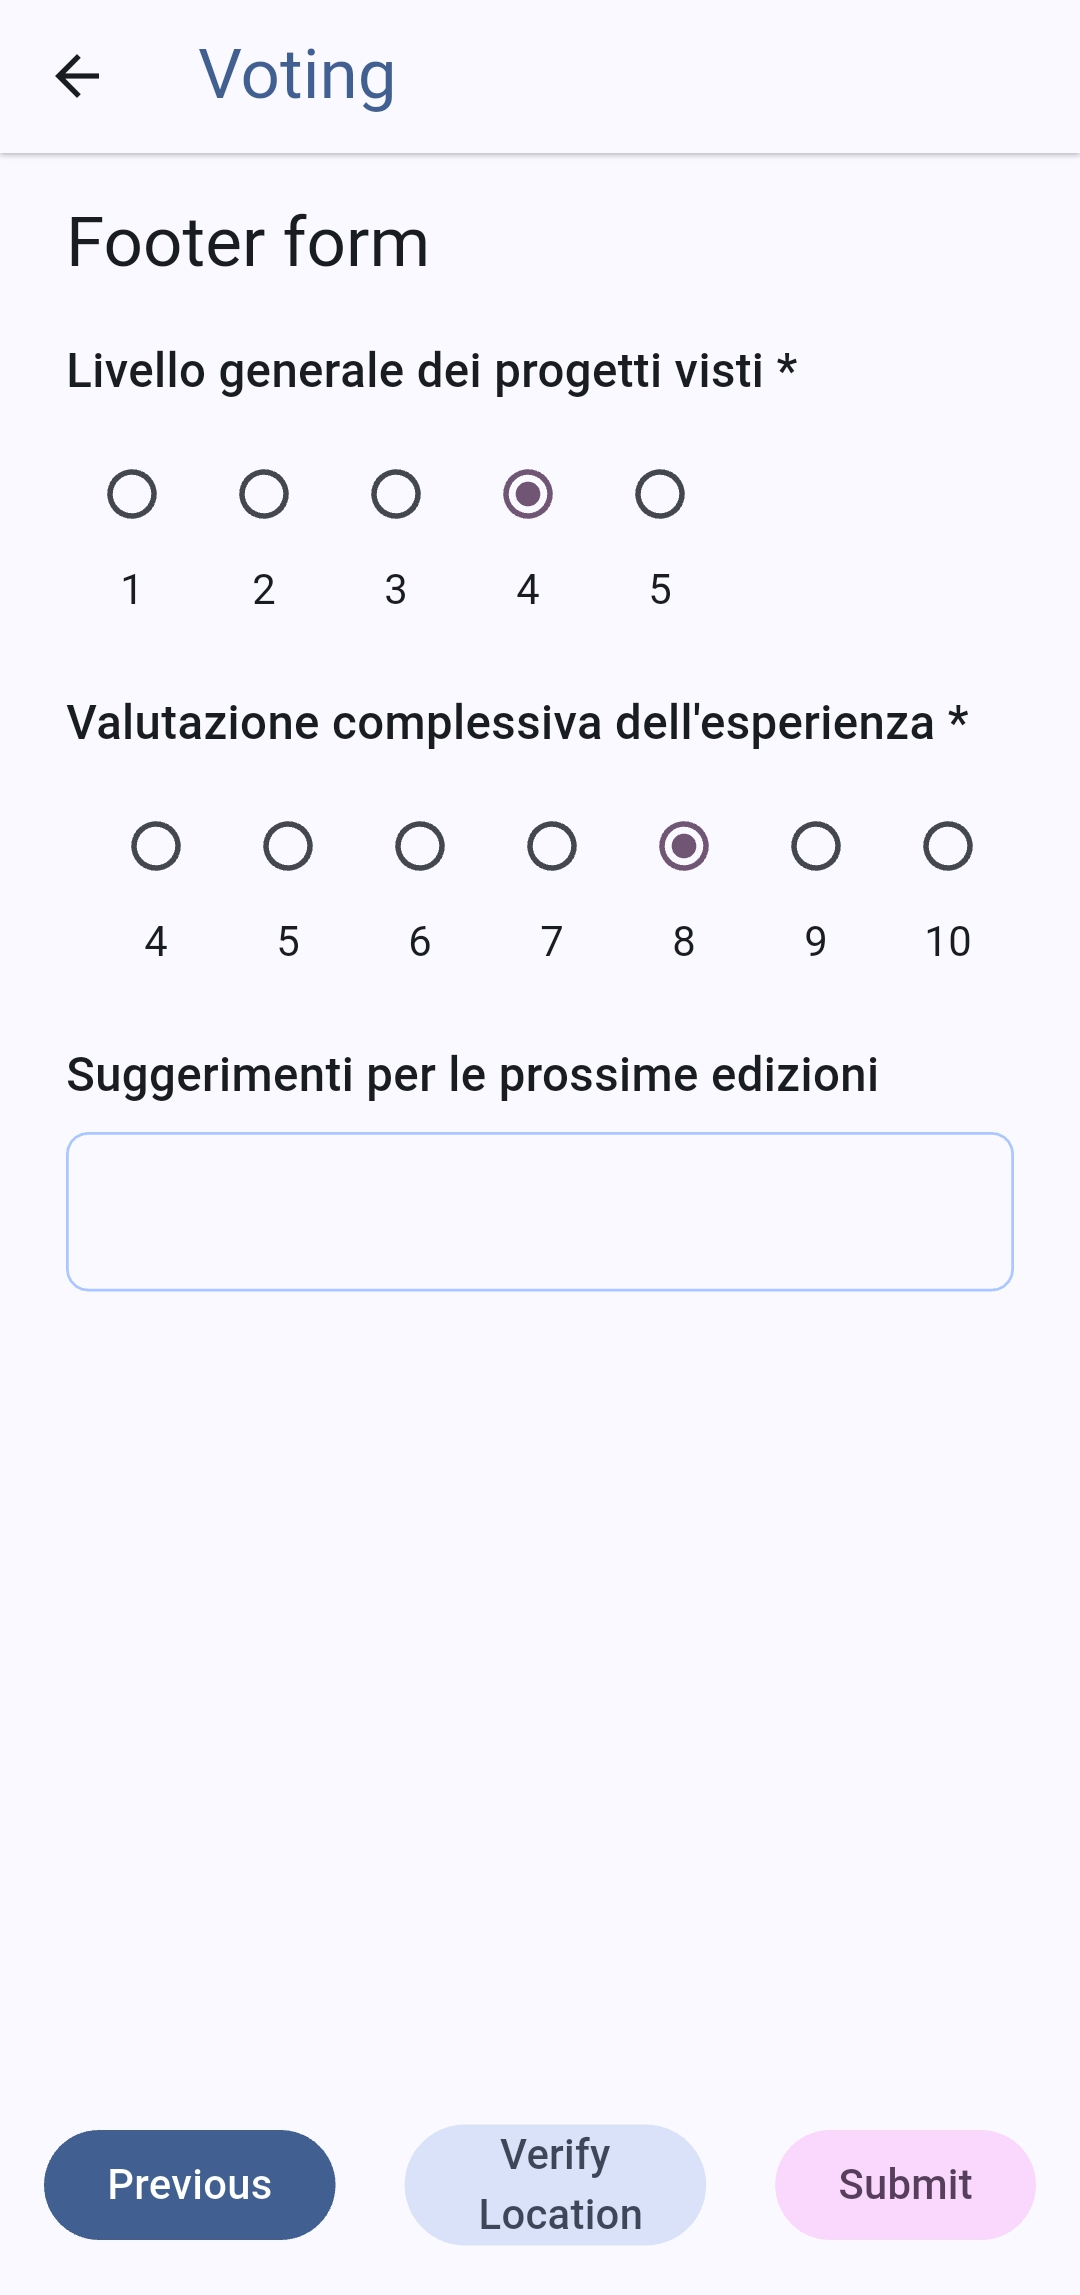
\includegraphics[width=\linewidth]{figure/juror-voting-session-footer}
        \subcaption{Votazione Campi Footer}
        \label{fig:voting_footer}
    \end{minipage}
    \caption{Le quattro fasi principali della procedura di votazione guidata per il giurato.}
    \label{fig:voting_procedure_flow}
\end{figure}

\subsection{Flusso del Giurato Semplice (Ospite)}\label{subsec:flusso-giurato-semplice}
Per massimizzare la flessibilità e abbassare la barriera d'ingresso, il sistema permette la partecipazione anche a giurati non registrati.
Questo flusso ``ospite'' è progettato per essere il più rapido e semplice possibile.

Il percorso inizia dalla pagina di \textbf{Sign In}, dove un pulsante dedicato permette di accedere come giurato semplice.
Invece di un form di registrazione, all'utente viene presentato un semplice popup che richiede solo l'inserimento di \textbf{nome e cognome}.
Una volta confermato, il sistema crea un account anonimo temporaneo e l'utente viene reindirizzato a una \textbf{Home Page minimale}, progettata esclusivamente per l'accesso alla sessione di voto.
Da qui, può scegliere se \textbf{scannerizzare il QR code} o \textbf{inserire manualmente il token} della giuria per accedere direttamente alla procedura di votazione, che è identica a quella del giurato nominato.

% --- FIGURE: Flusso Giurato Semplice (3 immagini affiancate) ---
\begin{figure}[H]
    \centering
    \begin{minipage}[t]{0.30\textwidth}
        \centering
        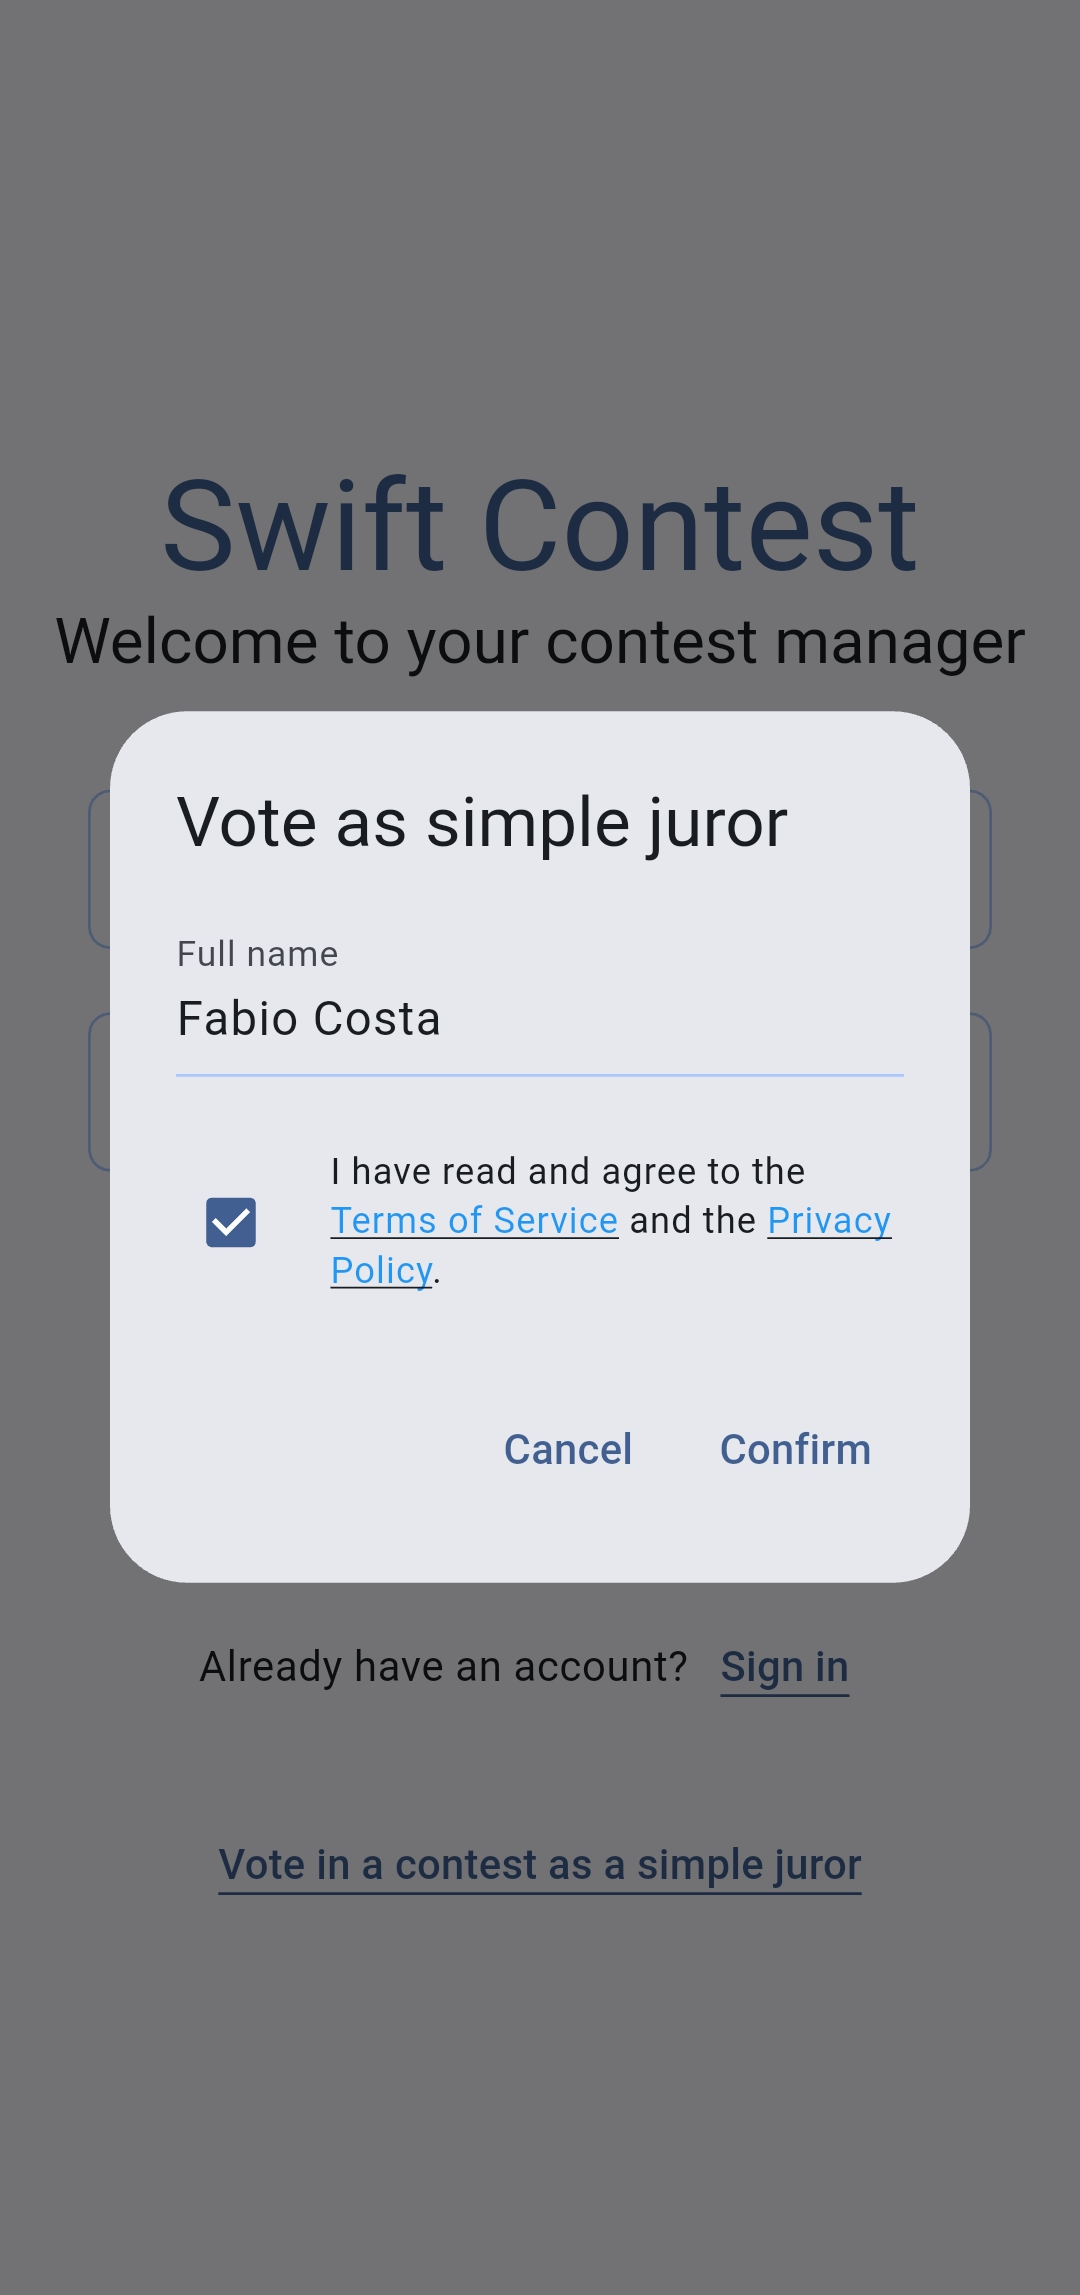
\includegraphics[width=\linewidth]{figure/simple-juror-sign-up}
        \subcaption{Accesso Ospite}
        \label{fig:simple_juror_entry}
    \end{minipage}
    \quad
    \begin{minipage}[t]{0.30\textwidth}
        \centering
        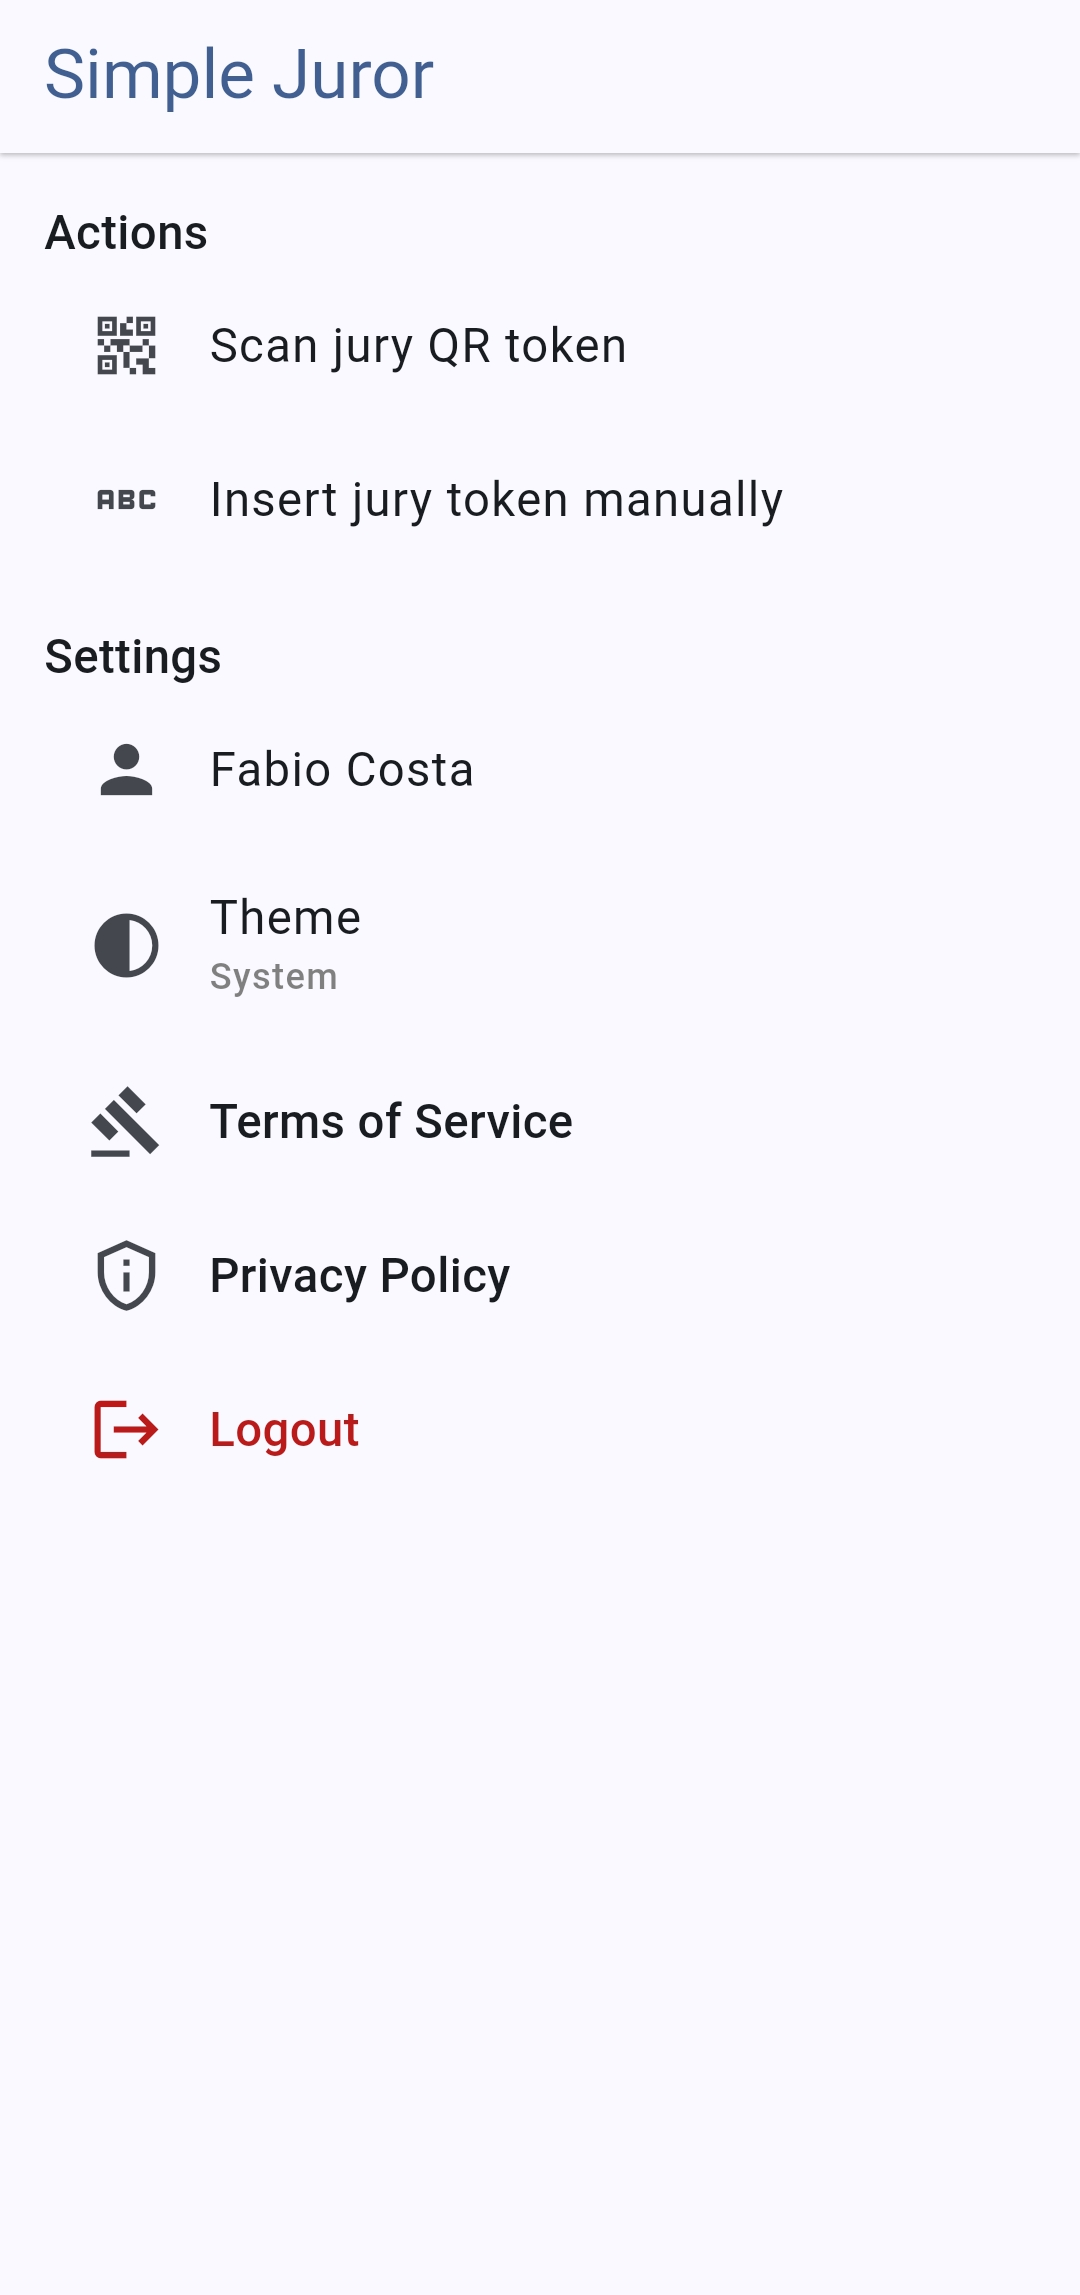
\includegraphics[width=\linewidth]{figure/simple-juror-home}
        \subcaption{Home Ospite}
        \label{fig:simple_juror_home}
    \end{minipage}
    \caption{I tre passaggi per l'accesso di un giurato semplice (ospite) alla piattaforma.}
    \label{fig:simple_juror_flow}
\end{figure}
